\documentclass[twocolumn,linenumbers]{aastex62}
%\documentclass{aastex62}
\usepackage{xspace}

%% The default is a single spaced, 10 point font, single spaced article.
%% There are 5 other style options available via an optional argument. They
%% can be envoked like this:
%%
%% \documentclass[argument]{aastex62}
%% 
%% where the layout options are:
%%
%%  twocolumn   : two text columns, 10 point font, single spaced article.
%%                This is the most compact and represent the final published
%%                derived PDF copy of the accepted manuscript from the publisher
%%  manuscript  : one text column, 12 point font, double spaced article.
%%  preprint    : one text column, 12 point font, single spaced article.  
%%  preprint2   : two text columns, 12 point font, single spaced article.
%%  modern      : a stylish, single text column, 12 point font, article with
%% 		  wider left and right margins. This uses the Daniel
%% 		  Foreman-Mackey and David Hogg design.
%%  RNAAS       : Preferred style for Research Notes which are by design 
%%                lacking an abstract and brief. DO NOT use \begin{abstract}
%%                and \end{abstract} with this style.
%%
%% Note that you can submit to the AAS Journals in any of these 6 styles.
%%
%% There are other optional arguments one can envoke to allow other stylistic
%% actions. The available options are:
%%
%%  astrosymb    : Loads Astrosymb font and define \astrocommands. 
%%  tighten      : Makes baselineskip slightly smaller, only works with 
%%                 the twocolumn substyle.
%%  times        : uses times font instead of the default
%%  linenumbers  : turn on lineno package.
%%  trackchanges : required to see the revision mark up and print its output
%%  longauthor   : Do not use the more compressed footnote style (default) for 
%%                 the author/collaboration/affiliations. Instead print all
%%                 affiliation information after each name. Creates a much
%%                 long author list but may be desirable for short author papers
%%
%% these can be used in any combination, e.g.
%%
%% \documentclass[twocolumn,linenumbers,trackchanges]{aastex62}
%%
%% AASTeX v6.* now includes \hyperref support. While we have built in specific
%% defaults into the classfile you can manually override them with the
%% \hypersetup command. For example,
%%
%%\hypersetup{linkcolor=red,citecolor=green,filecolor=cyan,urlcolor=magenta}
%%
%% will change the color of the internal links to red, the links to the
%% bibliography to green, the file links to cyan, and the external links to
%% magenta. Additional information on \hyperref options can be found here:
%% https://www.tug.org/applications/hyperref/manual.html#x1-40003
%%
%% If you want to create your own macros, you can do so
%% using \newcommand. Your macros should appear before
%% the \begin{document} command.
%%
\newcommand{\vdag}{(v)^\dagger}
\newcommand\aastex{AAS\TeX}
\newcommand\latex{La\TeX}

\newcommand{\Gray}{$\gamma$~ray\xspace}
\newcommand{\Grays}{$\gamma$~rays\xspace}
\newcommand{\GRays}{$\gamma$~Rays\xspace}
\newcommand{\gray}{$\gamma$-ray\xspace}
\newcommand{\unit}[1]{\,\mathrm{#1}\xspace}
\newcommand{\Fermi}{\emph{Fermi}\xspace}
\newcommand{\FermiLAT}{\emph{Fermi}~LAT\xspace}
\newcommand{\fermiLAT}{\emph{Fermi}-LAT\xspace}
\newcommand{\todo}[1]{\textbf{\textcolor{red}{#1}}}

%% Reintroduced the \received and \accepted commands from AASTeX v5.2
\received{\today}
\revised{???}
\accepted{???}
%% Command to document which AAS Journal the manuscript was submitted to.
%% Adds "Submitted to " the arguement.
\submitjournal{ApJ}

%% Mark up commands to limit the number of authors on the front page.
%% Note that in AASTeX v6.2 a \collaboration call (see below) counts as
%% an author in this case.
%
%\AuthorCollaborationLimit=3
%
%% Will only show Schwarz, Muench and "the AAS Journals Data Scientist 
%% collaboration" on the front page of this example manuscript.
%%
%% Note that all of the author will be shown in the published article.
%% This feature is meant to be used prior to acceptance to make the
%% front end of a long author article more manageable. Please do not use
%% this functionality for manuscripts with less than 20 authors. Conversely,
%% please do use this when the number of authors exceeds 40.
%%
%% Use \allauthors at the manuscript end to show the full author list.
%% This command should only be used with \AuthorCollaborationLimit is used.

%% The following command can be used to set the latex table counters.  It
%% is needed in this document because it uses a mix of latex tabular and
%% AASTeX deluxetables.  In general it should not be needed.
%\setcounter{table}{1}

%%%%%%%%%%%%%%%%%%%%%%%%%%%%%%%%%%%%%%%%%%%%%%%%%%%%%%%%%%%%%%%%%%%%%%%%%%%%%%%%
%%
%% The following section outlines numerous optional output that
%% can be displayed in the front matter or as running meta-data.
%%
%% If you wish, you may supply running head information, although
%% this information may be modified by the editorial offices.
\shorttitle{Gamma-ray variability of bright FSRQs}
\shortauthors{Meyer et al.}
%%
%% You can add a light gray and diagonal water-mark to the first page 
%% with this command:
% \watermark{text}
%% where "text", e.g. DRAFT, is the text to appear.  If the text is 
%% long you can control the water-mark size with:
%  \setwatermarkfontsize{dimension}
%% where dimension is any recognized LaTeX dimension, e.g. pt, in, etc.
%%
%%%%%%%%%%%%%%%%%%%%%%%%%%%%%%%%%%%%%%%%%%%%%%%%%%%%%%%%%%%%%%%%%%%%%%%%%%%%%%%%

%% This is the end of the preamble.  Indicate the beginning of the
%% manuscript itself with \begin{document}.

\begin{document}

\title{Characterizing the gamma-ray variability of the brightest flat spectrum radio quasars observed with the \emph{Fermi} LAT}

%% LaTeX will automatically break titles if they run longer than
%% one line. However, you may use \\ to force a line break if
%% you desire. In v6.2 you can include a footnote in the title.

%% A significant change from earlier AASTEX versions is in the structure for 
%% calling author and affilations. The change was necessary to implement 
%% autoindexing of affilations which prior was a manual process that could 
%% easily be tedious in large author manuscripts.
%%
%% The \author command is the same as before except it now takes an optional
%% arguement which is the 16 digit ORCID. The syntax is:
%% \author[xxxx-xxxx-xxxx-xxxx]{Author Name}
%%
%% This will hyperlink the author name to the author's ORCID page. Note that
%% during compilation, LaTeX will do some limited checking of the format of
%% the ID to make sure it is valid.
%%
%% Use \affiliation for affiliation information. The old \affil is now aliased
%% to \affiliation. AASTeX v6.2 will automatically index these in the header.
%% When a duplicate is found its index will be the same as its previous entry.
%%
%% Note that \altaffilmark and \altaffiltext have been removed and thus 
%% can not be used to document secondary affiliations. If they are used latex
%% will issue a specific error message and quit. Please use multiple 
%% \affiliation calls for to document more than one affiliation.
%%
%% The new \altaffiliation can be used to indicate some secondary information
%% such as fellowships. This command produces a non-numeric footnote that is
%% set away from the numeric \affiliation footnotes.  NOTE that if an
%% \altaffiliation command is used it must come BEFORE the \affiliation call,
%% right after the \author command, in order to place the footnotes in
%% the proper location.
%%
%% Use \email to set provide email addresses. Each \email will appear on its
%% own line so you can put multiple email address in one \email call. A new
%% \correspondingauthor command is available in V6.2 to identify the
%% corresponding author of the manuscript. It is the author's responsibility
%% to make sure this name is also in the author list.
%%
%% While authors can be grouped inside the same \author and \affiliation
%% commands it is better to have a single author for each. This allows for
%% one to exploit all the new benefits and should make book-keeping easier.
%%
%% If done correctly the peer review system will be able to
%% automatically put the author and affiliation information from the manuscript
%% and save the corresponding author the trouble of entering it by hand.

\correspondingauthor{Manuel Meyer}
\email{mameyer@stanford.edu}

\author[0000-0002-0738-7581]{Manuel Meyer}
\affil{W. W. Hansen Experimental Physics Laboratory, Kavli Institute for
Particle Astrophysics and Cosmology, Department of Physics and SLAC National Accelerator Laboratory, Stanford University, Stanford, CA
94305, USA}

\author{Jeffrey D. Scargle}
\affil{Space Sciences Division, NASA Ames Research Center, Moffett
Field, CA 94035-1000, USA}

\author{Roger Blandford}
\affil{W. W. Hansen Experimental Physics Laboratory, Kavli Institute for
Particle Astrophysics and Cosmology, Department of Physics and SLAC National Accelerator Laboratory, Stanford University, Stanford, CA
94305, USA}

%\author{The \emph{Fermi}-LAT Collaboration}
%\affiliation{Flying from a low Earth orbit}

%% Note that the \and command from previous versions of AASTeX is now
%% depreciated in this version as it is no longer necessary. AASTeX 
%% automatically takes care of all commas and "and"s between authors names.

%% AASTeX 6.2 has the new \collaboration and \nocollaboration commands to
%% provide the collaboration status of a group of authors. These commands 
%% can be used either before or after the list of corresponding authors. The
%% argument for \collaboration is the collaboration identifier. Authors are
%% encouraged to surround collaboration identifiers with ()s. The 
%% \nocollaboration command takes no argument and exists to indicate that
%% the nearby authors are not part of surrounding collaborations.

%% Mark off the abstract in the ``abstract'' environment. 
\begin{abstract}

Almost 10 years of $\gamma$-ray observations with the \emph{Fermi} Large Area Telescope (LAT) have revealed extreme  $\gamma$-ray outbursts from flat spectrum radio quasars (FSRQs), temporarily making these objects the brightest $\gamma$-ray emitters in sky. 
Yet, the location and mechanisms of the $\gamma$-ray emission remain elusive. 
We characterize long-term $\gamma$-ray variability and the brightest $\gamma$-ray flares of six FSRQs.
Consecutively zooming in on the brightest flares, which we identify in an objective way through Bayesian blocks and a hill-climbing algorithm, 
we find variability on sub-hour time scales and as short as minutes for  two sources in our sample (3C279, CTA102) and weak evidence for variability at time scales less than the Fermi satellite’s orbit of 95 minutes for PKS1510-089 and 3C454.3. 
This suggests extremely compact emission regions in the jet.
We do not find any signs for $\gamma$-ray absorption in the broad line region (BLR), which indicates that $\gamma$-rays are produced at distances greater than hundreds of gravitational radii from the central black hole. 
This is further supported by a cross-correlation analysis between $\gamma$-ray and radio light curves, which is compatible with a co-spatial production of $\gamma$~rays and emission at radio and mm wavelengths in 3C454.3 and CTA102.
The inferred locations of the $\gamma$-ray production zones are still consistent with the observed decay times of the brightest flares if the decay is caused by external Compton scattering with BLR photons. 
However, the minute-scale variability is challenging to explain in such scenarios.
%The gamma-ray light curves of these sources on different temporal scales provide us with a rich data set that can be compared to theoretical models of emission and particle cooling scenarios.

\end{abstract}

%% Keywords should appear after the \end{abstract} command. 
%% See the online documentation for the full list of available subject
%% keywords and the rules for their use.
\keywords{key word one --- key word two}

%% From the front matter, we move on to the body of the paper.
%% Sections are demarcated by \section and \subsection, respectively.
%% Observe the use of the LaTeX \label
%% command after the \subsection to give a symbolic KEY to the
%% subsection for cross-referencing in a \ref command.
%% You can use LaTeX's \ref and \label commands to keep track of
%% cross-references to sections, equations, tables, and figures.
%% That way, if you change the order of any elements, LaTeX will
%% automatically renumber them.
%%
%% We recommend that authors also use the natbib \citep
%% and \citet commands to identify citations.  The citations are
%% tied to the reference list via symbolic KEYs. The KEY corresponds
%% to the KEY in the \bibitem in the reference list below. 

\section{Introduction} \label{sec:intro}

More than half of the sources observed with the \Fermi Large Area Telescope (LAT) above 100\,MeV are active galaxies that produce particle outflows (jets) at almost the speed of light, which are closely aligned to the line of sight \citep[see, e.g., the third \Fermi source list, i.e., the 3FGL,][]{3fgl}.
%Yet, the exact mechanism and location of \gray production inside such jets of these so-called blazars remain a controversially discussed topic in the literature~\cite{Madejski:2016oqg}.
The broadband electromagnetic radiation observed from these so-called blazars spans decades in energy from radio frequencies up to very-high \gray energies. 
It is often described with purely leptonic or a mixture of leptonic and hadronic emission models, involving both intrinsic and external radiation fields~\cite[e.g.,][and references therein]{Madejski:2016oqg}.
%It is often explained with either purely leptonic or mixture of hadronic and leptonic emission models. 
%In leptonic models, the low energy part of the spectral energy distribution (SED) is caused by synchrotron emission of relativistic electrons in magnetic fields, whereas the high energy end of the SED is attributed to inverse Compton scattering of electrons with either the synchrotron emission or external radiation fields. 
%In leptonhadronic models, the high energy emission can be due to proton-synchrotron radiation, or the creation of particle cascades produced in interactions of cosmic rays with ambient gas and radiation fields. 
%In leptonic models, the emission is due to synchrotron emission and inverse Compton scattering of the electrons with synchrotron emission or external radiation fields. In leptohadronic models the high energy emission can be either due to proton-synchrotron radiation or emission produced in particle cascades, which are initiated by cosmic-ray interactions with gas and radiation fields.
A common assumption is that the radiation is emitted by freshly accelerated   particles localized in ``plasmoids''  that move down the jet at relativistic speeds,
 leading to a strong doppler boost of the observed emission. 
%Yet, the origin and location of such plasmoids remain unknown. 
Yet the origin, location even the very existence of such plasmoids are unknown.

Blazars display variability on timescales that can be as short as signal-to-noise limits allow and as long as the duration of the observations.
Flux doubling times as short as a few minutes have been observed at \gray energies in both BL Lac-type objects (BLL) and flat spectrum radio quasars (FSRQ) using  ground-based Cherenkov telescopes and the \FermiLAT~\cite[e.g.,][]{2007ApJ...669..862A,pks2155hess2007,pks1222magic2011,2013ApJ...762...92A,2014Sci...346.1080A,TheFermi-LAT:2016dss,2018ApJ...854L..26S}.
In these cases, causality arguments suggest extremely compact emission regions realized in, e.g., magnetic reconnection events, recollimation shocks, or magnetoluminescence~\cite[e.g.][]{Petropoulou:2016xat,Bodo:2017qqn,blandford:2017mag}.
In particular for FSRQs, the observation of \Grays beyond 10\,GeV suggests that these compact dissipation sites are located at distances of hundreds of Schwarzschild  radii from the central super massive black hole. 
Otherwise, the \gray emission should be strongly attenuated through pair production on UV and optical photons that are emitted by the accretion disk and broad emission line clouds and scttered by the inter-cloud medium.
Meeting these constraints is challenging for standard emission scenarios as extreme relativistic bulk motions of the plasma have to be invoked~\cite[e.g.,][]{TheFermi-LAT:2016dss}.  (For an alternative possibility see Sections~\ref{sec:blrabs}. and~\ref{sec:tcool})

After almost one decade of continuous all-sky observations, the \FermiLAT has accumulated a large sample of flares--\gray outbursts limited in time in which the source emission can increase typically by a factor of a few--from many FSRQs.
Our goal is to characterize flares and long-term behaviour of those FSRQs that have shown the brightest \gray flares over the course of the \Fermi mission. 
The most extreme flaring states enable us to perform a comprehensive search for \gray variability on time scales as short as minutes in order to investigate if such short variability -- and conversely compact emission sites -- is a common phenomenon in FSRQ flares. 
Evidence for minute-scale variability has already been discovered in LAT observations of 3C\,279~\citep{TheFermi-LAT:2016dss} and recently in CTA\,102~\citep{2018ApJ...854L..26S}, but searches in other sources have been unsuccessful~\citep{2017Galax...5..100N}.

The plethora of observed flares also enables us to perform a systematic study of the local temporal flare profiles, which could be diagnostic of particle injection, acceleration and, propagation.
\citet{2013MNRAS.430.1324N} investigated the brightest \gray flares in blazar in the first 4 years of LAT data.
The author found that, on average, flares have a slight tendency towards rise times being shorter than decay times; however, no flare showed extreme asymmetry. 
\citet{2010ApJ...722..520A}, on the other hand, characterized the blazars in terms of their power spectral density (PSD) on longer timescales using 11 months of data.
The authors found that the distribution of power-law slopes of the power spectra of bright blazars peak around $-1.2$ or $-1.3$, with a scatter marginally larger than the observational uncertainty.  That is to say intermediate between steep spectra (slope of $-2$, sometime called Brownian noise) and less steep (slope of $-1$, sometimes called flicker noise).
These analyses can be significantly extended with almost one decade of continuous \fermiLAT observations.

Additionally, the high signal-to-noise spectra during flares enable us to search for spectral absorption features due to the interaction of \Grays with BLR photons.
The detection of such features would locate the \gray emission region inside the BLR with important implications where particles dissipate their energy. 
Indeed, evidence for such absorption was reported in early  \fermiLAT observations~\citep{2010ApJ...717L.118P,2014ApJ...794....8S}, but a recent analysis of a large sample of over 100 FSRQs and more than 7\,years of \fermiLAT observations could not confirm this result~\citep{2018MNRAS.477.4749C}.
The absence of the absorption features can in turn be used to derive lower limits on the distance of the \gray emitting region to the central super-massive black hole. 

This paper is organized as follows. 
In Section~\ref{sec:data} we present the source selection and \FermiLAT data analysis. 
We investigate the global light curve properties in Section~\ref{sec:results-global}, before characterizing the temporal properties of the brightest flares in Section~\ref{sec:results-local}, which we identify by using an objective method.
%based on Bayesian blocks (BBs)~\citep{2013ApJ...764..167S} and one-dimensional group finding algorithms based on~\citet{1998ApJ...498..137E}.
We investigate the location of the \gray emitting region through searches for BLR absorption features in \gray spectra, a comparison between radiative cooling time scales and observed flare decay times, and a cross-correlations between long-term \gray and radio light curves in Section~\ref{sec:location}. 
We summarize our findings and conclusions in Section~\ref{sec:conclusion}.

\section{Source selection and data analysis}
\label{sec:data}

For our analysis, we select the FSRQs that show the brightest \gray flares as reported in the monitored source list\footnote{\url{https://fermi.gsfc.nasa.gov/ssc/data/access/lat/msl_lc/}}
with average daily fluxes $F \geqslant 10^{-5}\,\mathrm{cm}^{-2}\,\mathrm{s}^{-1}$ within ($1\,\sigma$ statistical uncertainties) above 100\,MeV.
This leaves us with 6 sources, listed in Table~\ref{tab:src-select}, together with their coordinates, redshift, and additional parameters taken from the literature such as black hole mass and luminosity of the $\mathrm{H}\beta$ line, a measure of the BLR luminosity.  
All of the sources in this selection have at least one 
flare that is suitable
%With the chosen flux threshold we ensure that we have at least one flare of each source in the sample that is suitable 
to search for intra-orbit variability and to derive high signal-to-noise spectra. 
All of the selected FSRQs are well known \gray emitters and individual flares from these objects have been studied in great detail~\citep[e.g.,][]{2010ApJ...714L..73A,2011ApJ...733...19T,2015ApJ...808L..48P,TheFermi-LAT:2016dss,2013ApJ...766L..11S,2015ApJ...809..164D,2018ApJ...854L..26S,2011ApJ...733L..26A}. 
As noted in the Introduction, two of the sources (3C279, CTA102) have already been shown to be variable on extremely short timescales~\citep{TheFermi-LAT:2016dss,2018ApJ...854L..26S}. 

Here, we will introduce a novel objective method to identify a large set of flares in order to conduct a comprehensive search for the short variability in our source sample.  
Furthermore, PKSB1222+216, 3C279, and PKS1510-089  are among the 7 FSRQs also detected above 100\,GeV with imaging air Cherenkov Telescopes~\citep{2011ApJ...730L...8A,2013A&A...554A.107H,2014A&A...569A..46A,2008Sci...320.1752M}. 

\begin{deluxetable*}{llccccccccc}
\tablewidth{0pt}
\tabletypesize{\scriptsize}
\tablecaption{ \label{tab:src-select}FSRQs selected for this study. }
\tablehead{
\colhead{Source name} &
\colhead{3FGL name} & 
\colhead{R.A.} & 
\colhead{DEC} & 
\colhead{Redshift} & 
\colhead{$\log_{10}(M_\bullet / M_\odot)$\tablenotemark{a}} &
\colhead{$L_\mathrm{disk}$\tablenotemark{a}} & \colhead{$L(\mathrm{H}\beta)$\tablenotemark{a}} &
\colhead{$\delta_\mathrm{D}$\tablenotemark{b}} &
\colhead{$\Gamma_\mathrm{L}$\tablenotemark{b}} &
\colhead{$\theta_\mathrm{obs}$\tablenotemark{b}}\\
{} & {} & \colhead{[deg]} & \colhead{[deg]} & {} & {} & \colhead{$[10^{46} \mathrm{ergs}\,\mathrm{s}^{-1}]$} & \colhead{$[10^{43} \mathrm{ergs}\,\mathrm{s}^{-1}]$} &
{} & {} & \colhead{[deg]} 
}
\startdata
PKS\,B1222+216 & 3FGL\,J1224.9+2122 & 186.226  & 21.382 & 0.432 & 8.87\tablenotemark{c} & $1.61$ &  $2.79 \pm 0.56$\tablenotemark{d} & $7.4 \pm 2.1$ & $13.9\pm2.1$ & $5.6\pm1.0$\\
3C\,273 &	3FGL\,J1229.1+0202 & 187.266  & 2.051 & 0.158 & 	8.92 &	6.11 & 	15.40 & $4.3\pm1.3$ & $8.5\pm2.2$ & $6.4\pm2.4$ \\
3C\,279 & 3FGL\,J1256.1-0547 & 194.045  & $-5.786$ & 0.5362 	&	8.28 &	1.11 &	1.73 & $18.3\pm1.9$ & $13.3\pm0.6$ & $1.9\pm0.6$\\
PKS\,1510-089 &	3FGL\,J1512.8-0906 & 228.210  & $-9.106$ & 0.360 & 8.20 & 1.13 & 1.77 & $35.3\pm 4.6$ & $22.5\pm3.3$ & $1.2\pm0.3$\\
CTA\,102 & 3FGL\,J2232.5+1143 & 338.158  & 11.728 & 1.037 & 8.93\tablenotemark{c} & 4.00  &	8.93 $\pm$  6.00\tablenotemark{e} & $30.5\pm3.3$ & $21.7\pm1.3$ & $1.6\pm0.4$\\
3C\,454.3 & 3FGL\,J2254.0+1608 & 343.493  & 16.149 & 0.859 & 	8.83 &	7.19 & 	19.00 & $24.4\pm3.7$ & $13.8\pm1.4$ & $0.7\pm0.4$\\
\enddata
\tablenotetext{a}{Taken from \citet{2006ApJ...637..669L} if not noted otherwise.}
\tablenotetext{b}{Average jet values taken from \citet{2017ApJ...846...98J}.}
\tablenotetext{c}{From \citet{2014Natur.510..126Z}.}
\tablenotetext{d}{From \citet{2012RMxAA..48....9T}.}
\tablenotetext{e}{\citet{2012RMxAA..48....9T} give the $L$(CIV) with $(255.7 \pm 17.2)\times10^{43}\mathrm{ergs}\,\mathrm{s}^{-1}$ and Eq.~7 from \citet{2006ApJ...637..669L} is used to convert this to $L$(H$\beta$).}
\tablecomments{The reported source positions are derived from 
our \gray analysis. $M_\bullet$ denotes the black hole mass, $L_\mathrm{disk}$ the accretion disk luminosity, $L(\mathrm{H}\beta)$ is the luminosity of the $\mathrm{H}\beta$ emission line, $\delta_\mathrm{D}$ denotes the relativistic Doppler boost factor, $\Gamma_\mathrm{L}$ is the bulk Lorentz factor, and $\theta_\mathrm{obs}$ is the angle between the jet axis and the line of sight. }

\end{deluxetable*}

\subsection{Data selection}

Our goal is characterize both the long term \gray behavior of the selected FSRQs as well as the brightest flares.
To this end, we select \Grays that have been measured with the \FermiLAT between August 4, 2008, and January 30, 2018, yielding data over an interval of 114\,months, or almost 9.5\,years.
The \FermiLAT is a pair conversion telescope designed to measure \Grays with energies between 20\,MeV to above 300\,GeV~\citep{2009ApJ...697.1071A}.

We follow the standard data selection recommendations\footnote{\url{https://fermi.gsfc.nasa.gov/ssc/data/analysis/documentation/Cicerone/Cicerone_Data_Exploration/Data_preparation.html}} and  restrict ourselves to \Grays in the energy range between 100\,MeV and 316\,GeV. 
Below 100\,MeV the effective area of the LAT quickly decreases and the point spread function increases to above $\sim 6^\circ$\footnote{See, e.g., \url{http://www.slac.stanford.edu/exp/glast/groups/canda/lat_Performance.htm}} making a point source analysis challenging. 
Since FSRQs usually have soft \gray spectra, we do not expect significant detection of these sources above our chosen maximum energy.

To mitigate contamination of \Grays originating from the Earth Limb, we further limit the sample to events that have arrived at a zenith angle less than $90^\circ$ and we excise periods of bright GRBs and solar flares that have been detected with a test statistic $\mathrm{TS} > 100$.
The test statistic is defined as $\mathrm{TS} = -2\ln(\mathcal{L}_1 / \mathcal{L}_0)$, i.e., the log-likelihood ratio between the the maximized likelihoods $\mathcal{L}_1$ and $\mathcal{L}_0$ for the hypotheses with and without an additional source, respectively~\citep{mattox1996}.
We use the latest \texttt{Pass 8} instrumental response functions and Monte Carlo simulations~\citep{pass8} and select \Grays that pass the \texttt{P8R2 SOURCE} event selection. 
For each source we analyze a $10^\circ \times 10^\circ$ Region Of Interest (ROI) centered on the position of each source as provided in the third \fermiLAT point source catalog \citep[3FGL,][]{3fgl}.
We choose a spatial binning of $0.1^\circ$ per pixel and 8 energy bins per decade. 

\subsection{ROI optimization}
\label{sec:roi}

Our analysis proceeds iteratively, starting from the full time range and zooming in on bright flares and shorter time scales (see Section~\ref{sec:zoom}).
In a first step, we optimize the global \gray model of each ROI using the \textit{Fermi Science Tools} version 11-05-03\footnote{\url{http://fermi.gsfc.nasa.gov/ssc/data/analysis/software}} and \textsc{fermipy}, version 0.16.0+188\footnote{\url{http://fermipy.readthedocs.io}}~\citep{fermipy}.
The initial model consists of all \gray point sources within $15^\circ$ from the ROI center included in the 3FGL as well as the standard templates for isotropic and Galactic diffuse emission.\footnote{For the Galactic diffuse emission we use the file gll\_iem\_v06.fits and the file iso\_P8R2\_SOURCE\_V6\_v06.txt for the isotropic diffuse component, see: \url{ http://fermi.gsfc.nasa.gov/ssc/data/access/lat/BackgroundModels.html}}
After an initial optimization, we free the spectral normalization of sources that are within $10^\circ$ from the ROI center or that are detected with $\mathrm{TS} > 50$.
The spectral shape parameters such as power-law indices, curvature, or exponential cut-off energies are free to vary for sources within $5^\circ$ from the ROI center. 
We freeze all spectral source parameters for sources detected with $\mathrm{TS} < 1$ or if the number of predicted photons is less than $10^{-3}$ to the values provided in the 3FGL. 
The normalizations of the diffuse backgrounds are left free during the fit, together with the spectral index of the Galactic diffuse background template.
After the fit has converged successfully, 
we relocalize the central \gray source and re-fit all spectral model parameters. The relocalized source positions are provided in Table~\ref{tab:src-select}.
After this step, we generate a $\mathrm{TS}$ map to search for additional point sources. For each pixel in the ROI, we add a putative point source with a power-law spectrum with index $\Gamma = 2$ and calculate its $\mathrm{TS}$. If  $\sqrt{\mathrm{TS}} \geqslant 5$, we permanently add the source at the position of the highest $\mathrm{TS}$ value and re-optimize the spectral parameters for the whole ROI. This step is repeated until no further sources are found.

With the best-fit model for each ROI, we compute the \gray light curves for the FSRQs with an initial binning of 7~days. 
In each light curve bin, we leave spectral parameters free during the fit for sources within $3^\circ$ from the ROI center and additionally the normalizations of the Galactic and isotropic emission. If any of these sources have $\mathrm{TS} < 1$ or the number of predicted photons is less than $10^{-3}$, their parameters are fixed to the average values.

\subsection{Zooming in on bright flares using an objective method to identify different activity states}
\label{sec:zoom}

The 9.5 year light curves for all considered FSRQs are shown in Figure~\ref{fig:weekly}. If the source is detected with $\mathrm{TS} < 9$ within one time bin or the flux in one bin is equal or smaller than its statistical uncertainty $F_i \leqslant \sigma_i$, we show upper limits\footnote{We avoid 
problems with incorporating upper limits by simply ignoring them, because the BB algorithm does not require evenly spaced data. At these gaps there
are just two possibilities:
(1) a single block spans the gap,
or 
(2) one block stops at the beginning of
the gap and another starts at the end.
The former indicates that the flux levels
before and after the gap are the same,
the latter that they are not.
In neither case is there definitive 
information about the level in the
gap itself.}
at the $2\,\sigma$ confidence level instead (open symbols).

The average source fluxes with their 1$\,\sigma$ statistical uncertainties, $\overline{F} \pm \sigma_{\overline{F}}$, derived from the likelihood maximization over the full 9.5\,years are shown as gray bands. 
These flux measurements and uncertainties determine the optimal step-function representations of the light curves (shown as orange lines) using the Bayesian Block (BB) 
algorithm ~\citep[][]{2013ApJ...764..167S} maximizing the overall fitness function appropriate to \textit{point measurements}.
From all possible partitions of the data into blocks this algorithm finds the unique one maximizing the total fitness of the resulting step-function model.


These blocks provide an objective way to detect significant local variations in the light curve.
Several strong flares exceeding the average flux level are easily identified from this block representation. 

%%% Full light curve %%%
\begin{figure*}
    \centering
    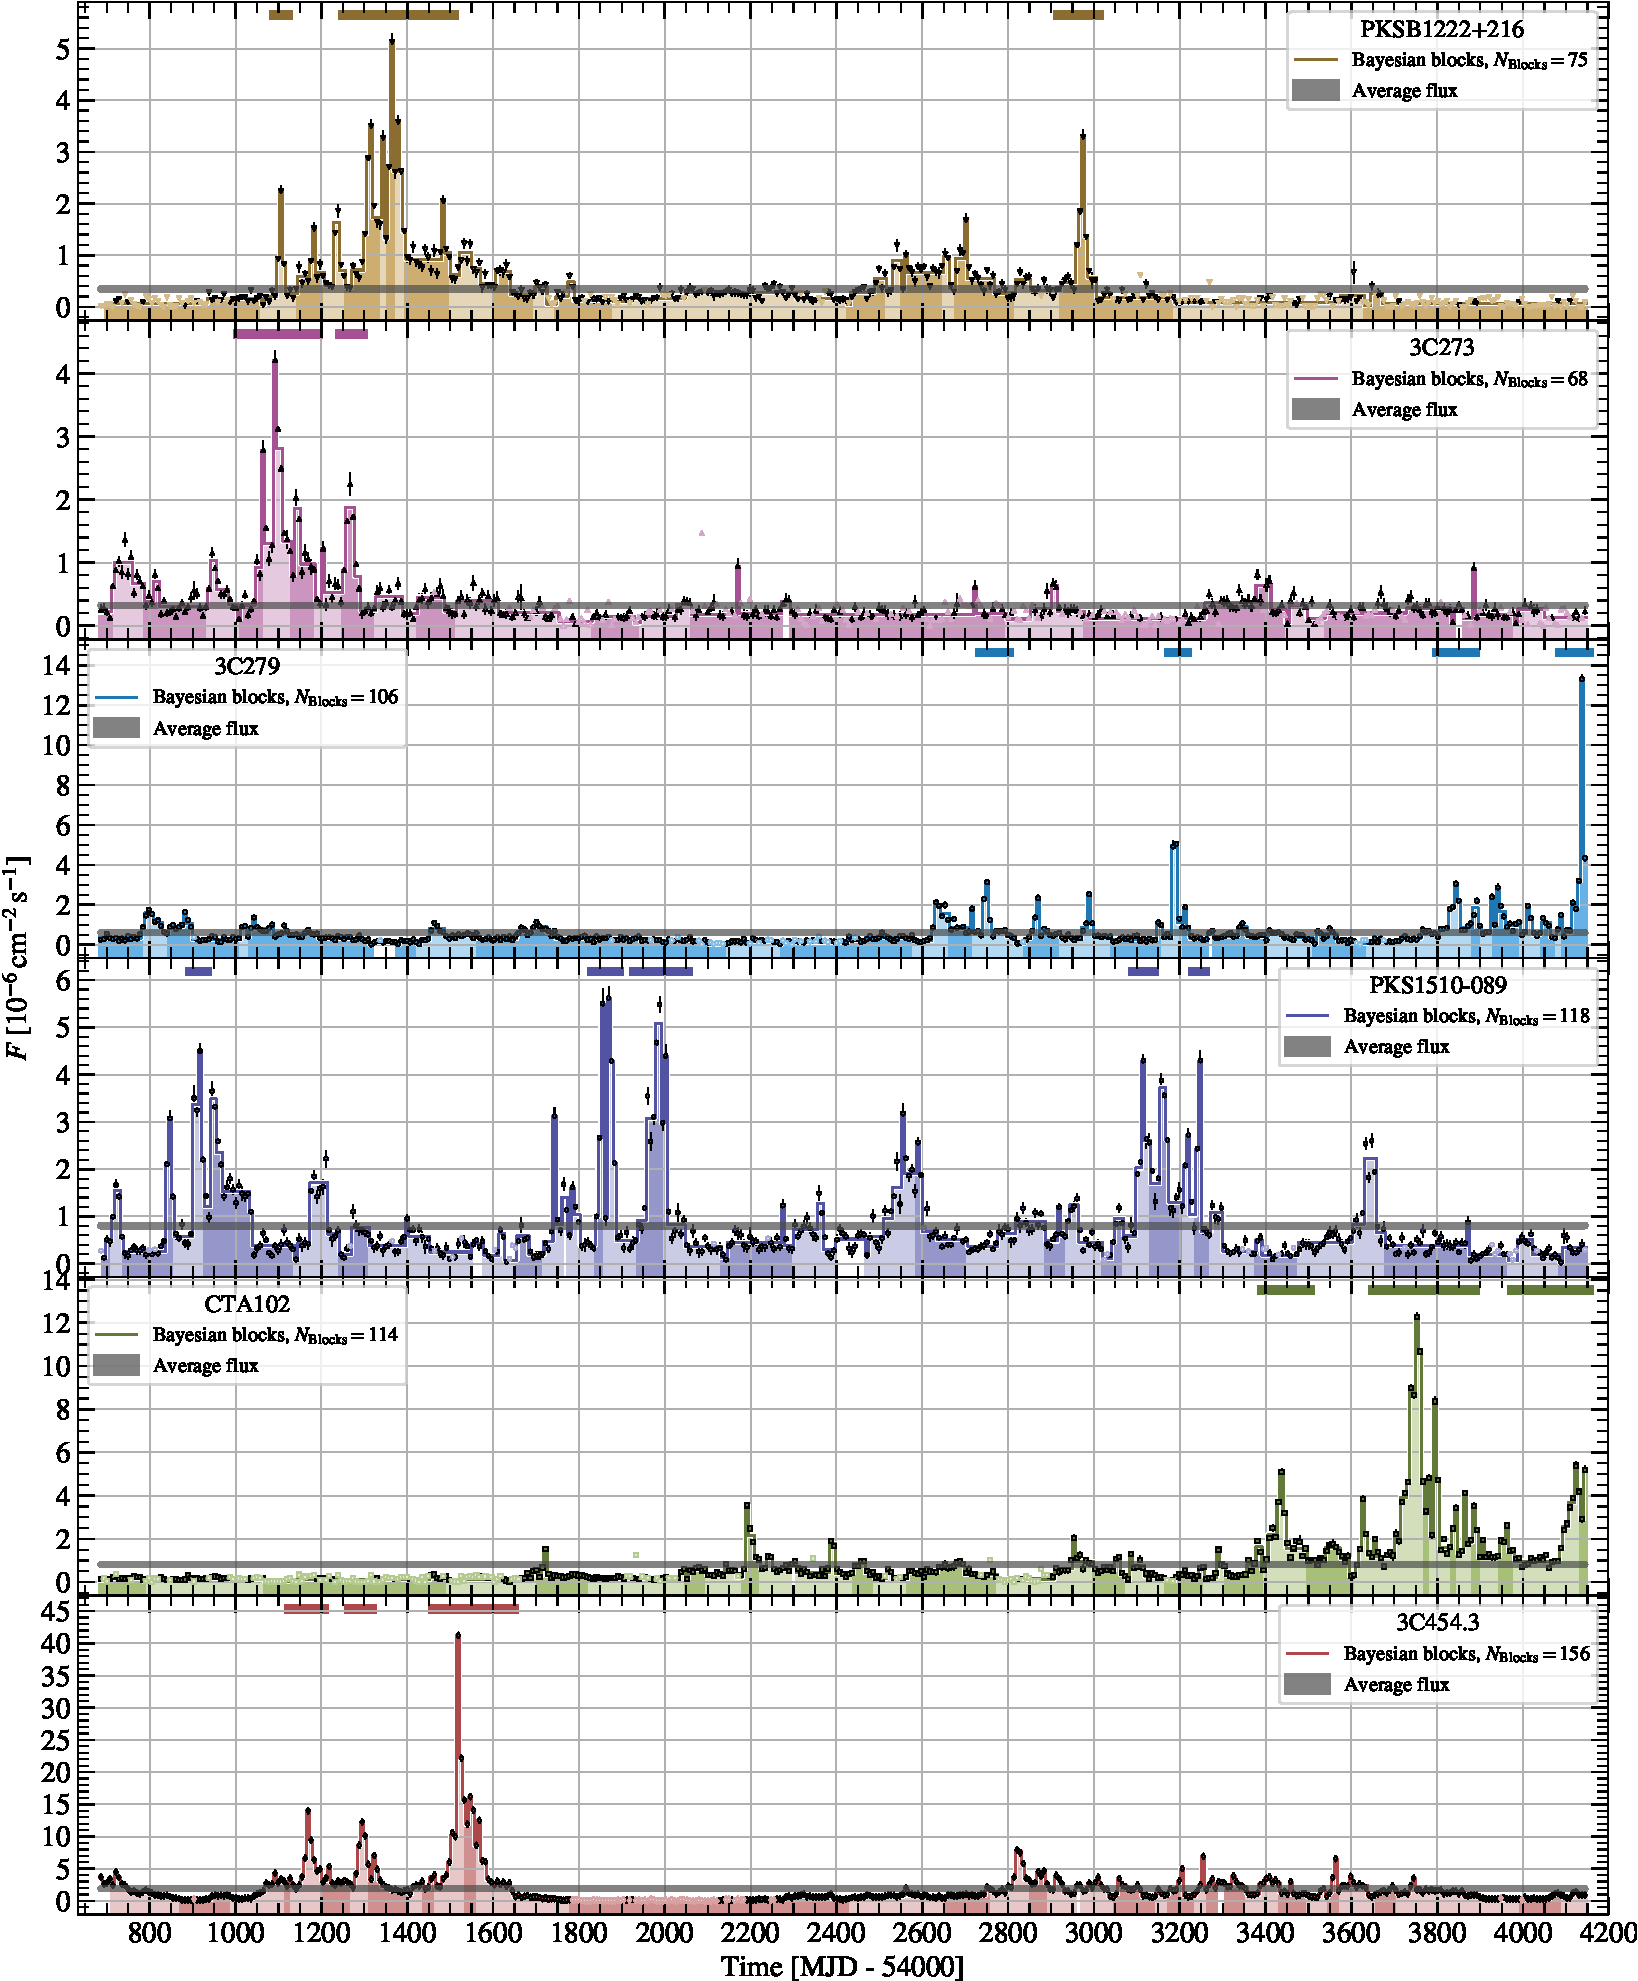
\includegraphics[width = .9\linewidth]{figures/lc_weekly_tsmin9.pdf}
    \caption{\gray light curves with weekly binning for the considered FSRQs. Open symbols denote upper limits at the $2\,\sigma$ confidence level. The solid lines show the BBs and the shaded regions represent the identified HOP groups. The horizontal lines denote the time intervals identified as bright flares for which we derive light curves with finer binning.}
    \label{fig:weekly}
\end{figure*}

There is no generally accepted consensus on the best way to determine which data points belong to a flaring state and which characterize the quiescent level. \citet{2013MNRAS.430.1324N} suggests a simple definition that a flare is a continuous time interval associated with a flux peak in which the flux is larger than half the peak flux value. 
This definition is intuitive, however, and it is unclear how to treat overlapping flares and identify flux peaks in an objective way. 
Here we use a simple two step procedure tailored to the block representation: (1) identify a block that is higher than both the previous and subsequent blocks as a \textit{peak}; (2) proceed downward from the peak in both directions as long as the blocks are successively lower.
The two resulting monotonically decreasing sets of adjacent blocks are analogous to the \textit{watershed} concept of topological data analysis.
In fact this approach was suggested by the 
HOP algorithm~\citep{1998ApJ...498..137E}, which is based on a bottom-up hill climbing concept of great use in higher dimensions \citep[e.g.,][]{2011ApJ...727...48W}.

The time series segments shown in 
Figure~\ref{fig:weekly} as dark and light shaded  areas are the result of feeding
the block representations of the light curves to the HOP algorithm.
The combination of BB and the HOP algorithm provides an objective way to split a light curve into groups of quiescent and flaring episodes; we will refer to one connected flare episode as a \emph{HOP group} of consecutive BBs.

We iteratively zoom in on time ranges with bright \gray activity by identifying HOP groups where the peak BB fulfills the condition $F_{BB} \geqslant F_\mathrm{max} =  5\times\overline{F}$ and include adjacent blocks within the group with $F_{BB} \geqslant F_\mathrm{min} = \overline{F}$. 
This relatively conservative definition 
gives reliable group shape information 
at the cost of 
slightly underestimating the extent of the
groups and overestimates that of the quiescent 
intervals.
Furthermore, we prefer a criterion based on peak flux rather than, for instance, integrated flare luminosity, because this approach promises the most straightforward way to find those time ranges with sufficient photon statistics to search for short timescale flux variations and exponential cut-offs due to \gray absorption. 
% Overlapping -- why overlapping?
The indicated adjacent time intervals are combined into one time range and then extended by one time bin on either side.
For the identified time span, we re-optimize the spectral model of the ROI in the same way as described in Section~\ref{sec:roi} but without re-localizing the central FSRQ or adding new point sources. 
The results of the best-fit spectra for the different time ranges are provided in Appendix~\ref{sec:avg-spec}.
Subsequently, we calculate a light curve with finer binning and again select the time ranges of the highest \gray activity. We repeat this procedure twice, down to a binning equal to the Good Time Intervals (GTIs), of the \Fermi satellite, which correspond to one passage of the source through the field of view of the satellite during one $\sim$ 95 minute orbit.
The choices of time binnings and values for $F_\mathrm{max}$ and $F_\mathrm{min}$ are summarized in Table~\ref{tab:zoom} together with the number of identified high \gray activity states (which might consists of several flares as indicated by the HOP groups).

The values of the threshold fluxes $F_\mathrm{max}, F_\mathrm{min}$ is somewhat arbitrary and are a compromise between including as many flares as possible but keeping the overall number of flares manageable. Note, that the sole purpose of this exercise is to select the brightest flares for further analysis; consideration of a more
complete statistical sample is postponed to 
the future.

The identified time ranges for the weekly light curves are plotted as colored horizontal solid lines in Figure~\ref{fig:weekly}.
The intermediate daily light curves are provided in Figure~\ref{fig:daily}.
Figure~\ref{fig:gti} shows the GTI (equivalent to orbital) light curves with exponential fits of flare profiles that we will discuss in Section~\ref{sec:results-local}. 
The source exposure can vary significantly between two adjacent orbits, as the satellite rocks between the celestial north and south pole between orbits. 
This explains the large error bars on some of the time bins of the GTI light curves.

\begin{deluxetable}{cccc}
\tablewidth{1\linewidth}
\tablecaption{ \label{tab:zoom} Thresholds for BB fluxes in one HOP group to select time ranges of high \gray activity together with selected time binning and number of selected time ranges.
}
\tablehead{\colhead{Binning} & \colhead{$F_\mathrm{min}$} & \colhead{$F_\mathrm{max}$} & \colhead{$N_\mathrm{time~ranges}$}}
\startdata
7 days & $\overline{F}$ & $5\times\overline{F}$ & 20\\
1 day & $\overline{F}$ & $\mathrm{max}(10^{-5}\,\mathrm{cm}^{-2}\,\mathrm{s}^{-1}, 1.5 \times \overline{F})$\tablenotemark{a} & 21\\
GTI & $\overline{F}$ & $2\times\overline{F},~\mathrm{TS} \geqslant 150$\tablenotemark{b} & 7\\
%Sub-GTI & -- & -- & --\\
\enddata
\tablenotetext{a}{We choose here the absolute flux (rather than the flux relative to the average) as a threshold in order to be consistent with our initial source selection. However, because of the high avergage flux of 3C454.3, we also include the max argument. If $F_\mathrm{max} = 1.5 \times \overline{F}$ we set $F_\mathrm{min} = 10^{-5}\,\mathrm{cm}^{-2}\,\mathrm{s}^{-1}$. }
\tablenotetext{b}{Motivated from the high $\mathrm{TS}$ found for the flare of 3C\,279~\citep{TheFermi-LAT:2016dss}, we also demand that at least one GTI of each HOP group is detected with $\mathrm{TS} \geqslant 150$ in order to ensure enough statistics to search for variability on time scales of minutes.}
\tablecomments{The criteria are applied to all sources. Furthermore, if no interval fulfills the $F_\mathrm{BB} \geqslant F_\mathrm{max}$ criterion for the weekly or daily light curves, we include the HOP group of the maximum flux if that flux exceeds $5\times10^{-6}\,\mathrm{cm}^{-2}\,\mathrm{s}^{-1}$, i.e., we change $F_\mathrm{max}$ to the maximum value $F_\mathrm{BB}$.}
\end{deluxetable}

In a last step, we derive light curves on sub-GTI time scales. 
The time bin size is calculated from the adaptive binning method of \citet{lott2012}, where we choose bins of constant flux uncertainty of $\sim20\,\%$. 
In this step, we use the space craft information in time steps of 1\,s instead of 30\,s. Additionally, we compute the effective area in 5 bins of the azimuthal spacecraft coordinates since on such short time scales the exposure dependence on the azimuth should not be averaged over.\footnote{See \url{https://fermi.gsfc.nasa.gov/ssc/data/analysis/scitools/help/gtltcube.txt}}
We discuss these light curves in Section~\ref{sec:sub-gti}.


%%% Daily light curves %%%%%%%%%
\begin{figure*}
    \centering
    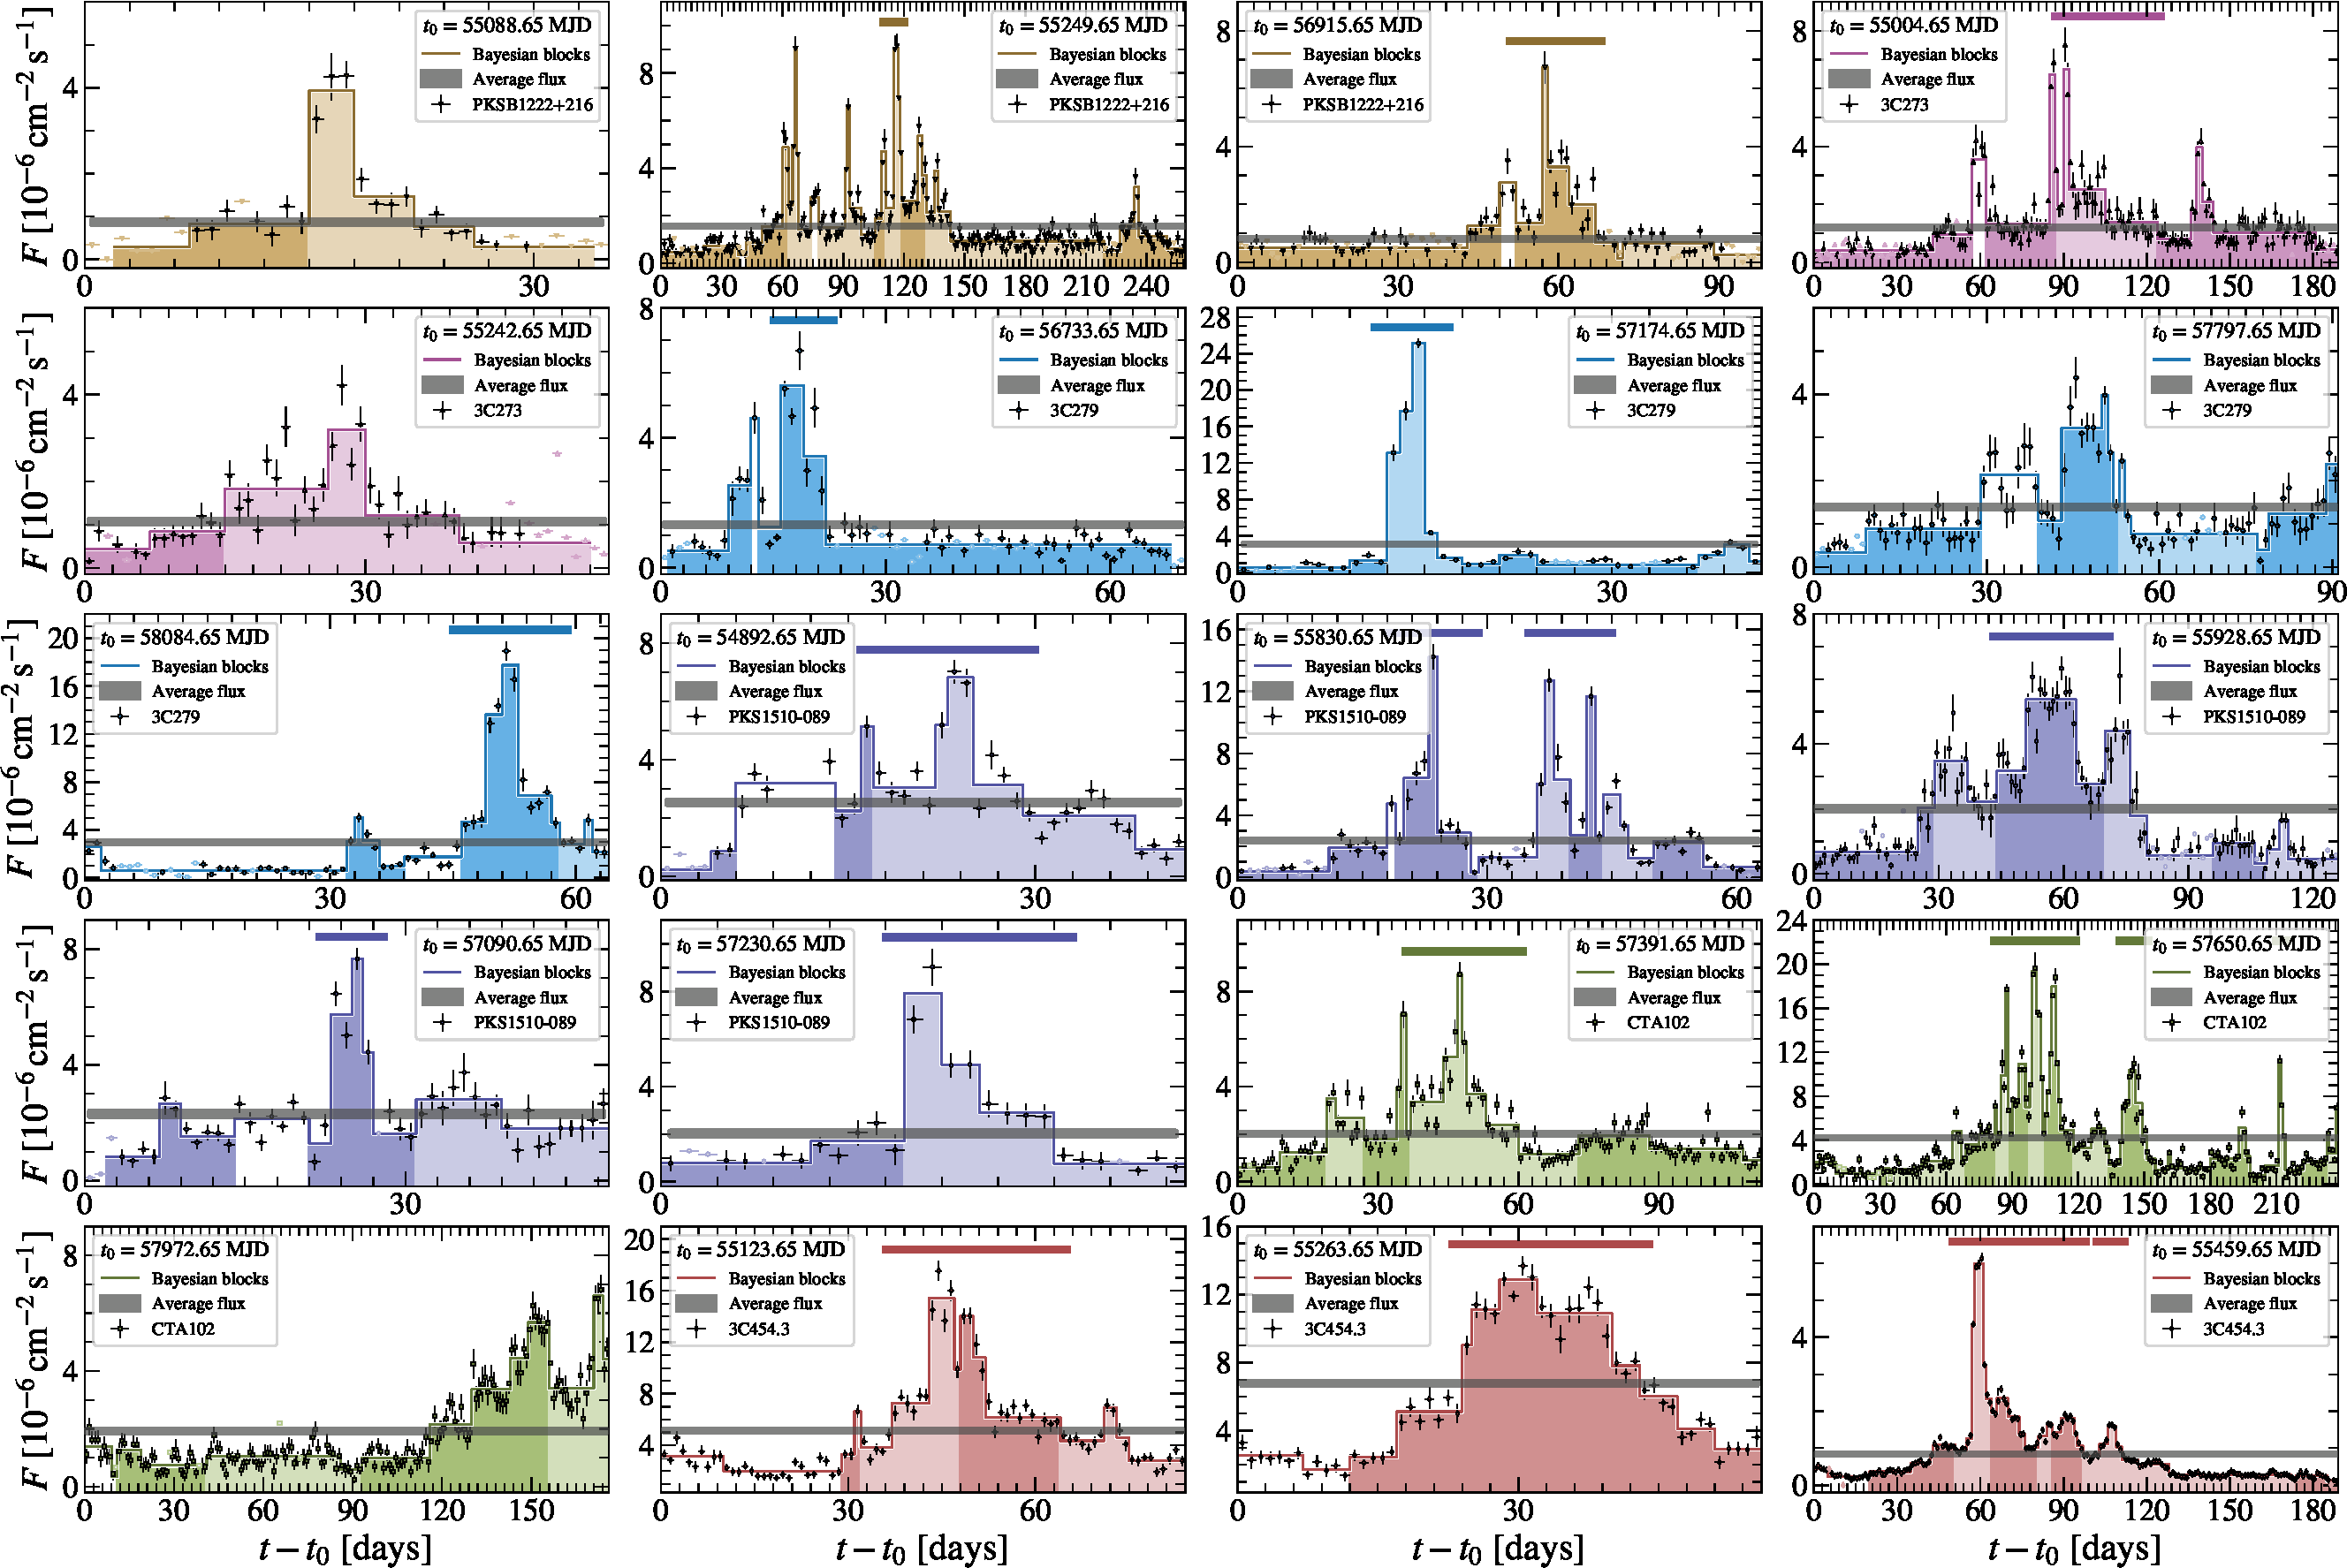
\includegraphics[width = .99\linewidth]{figures/lc_daily_tsmin9.pdf}
    \caption{\label{fig:daily} Light curves with daily binning for the selected time ranges (horizontal lines in Figure~\ref{fig:weekly}). Symbols and lines are the same as in Figure~\ref{fig:weekly}. 
    As stated in Table~\ref{tab:zoom}, if all BB fluxes fail the criterion $F_{BB} \geqslant \mathrm{max}(10^{-5}\,\mathrm{cm}^{-2}\,\mathrm{s}^{-1}, 1.5 \bar{F})$, we include the HOP group with the maximum flux of the interval if that flux is above $5\times 10^{-6}\,\mathrm{cm}^{-2}\,\mathrm{s}^{-1}$. This is the case, e.g., for last two intervals of PKSB1222+216 and the first interval of 3C273 (last three panels of the top row).}
\end{figure*}
%%%%%%%%%%%%%%%%%%%%%%%%%%%%%%%%

\section{Results for global light curve properties}
\label{sec:results-global}
We first present results derived from the weekly \gray light curves spanning the full 9.5\,year time range, which we refer to as \emph{global light curve properties}, before deriving results from the local light curves on GTI and sub-GTI time scales in Section~\ref{sec:results-local}.

From the weekly light curves in Figure~\ref{fig:weekly}, it is evident that the FSRQs show strong flares that exceed the average flux by a factor of a few, while the quiescent level is relatively stable. 
Such behavior is typical for FSRQs~\citet{} and we 
further quantify it by calculating the flux distribution, $dN/dF$, of the weekly fluxes for bins with $\mathrm{TS} \geqslant 9$ and $F_i \geqslant \sigma_i$. 
The results are shown in Figure~\ref{fig:fluxpdf}. The flux bins are chosen according to the algorithm of~\citet{knuth2006} and the error bars are calculated under the assumption that the observed weekly fluxes, $F_i$, $i = 1,\ldots,n$, are Gaussian-distributed numbers with standard deviation equal to the measurement uncertainty $\sigma_i$.\footnote{
With this assumption, the uncertainty to find $x$ entries in the $j$-th flux bin of width $\Delta F_j = F_{\mathrm{hi},j} - F_{\mathrm{lo},j}$ is given by the sum of Bernoulli probabilities $p_{ij}$, $\sum_{i = 1}^n p_{ij}(1-p_{ij})$, where $p_{ij} =  \left[\mathrm{erf}\left((F_{\mathrm{hi},j} - F_i) / \sqrt{2\sigma_i^2}\right) - \mathrm{erf}\left(((F_{\mathrm{lo},j} - F_i) / \sqrt{2\sigma_i^2}\right)\right]/2$, and $\mathrm{erf}$ is the error function.
}
We fit the flux distribution with a smoothly broken power law (BPL) of the form 
\begin{equation}
    \frac{dN}{dF} = N_0 \left( \frac{F}{F_0}\right)^{\alpha_\mathrm{low}}
        \left( 1 - \left(\frac{F}{F_\mathrm{br}}\right)^s \right)^{\frac{\alpha_\mathrm{high} - \alpha_\mathrm{low}}{s}},
        \label{eq:dndf}
\end{equation}
with the smoothing factor $s$ fixed to 3. 
The results of a $\chi^2$ minimization are summarized in Table~\ref{tab:global}.
Generally, below the break flux $F_\mathrm{br}$, the flux distribution is flat, $\alpha_\mathrm{low}\sim 0$.
Above $F_\mathrm{br}$, 
%which indicates the maximum flux of the quiescent level and 
which lies between $\sim2\times10^{-7}$ and $\sim2\times10^{-6}\,\mathrm{cm}^{-2}\mathrm{s}^{-1}$, $dN/dF$ declines exponentially with power-law indices $\alpha_\mathrm{high} \lesssim -2.2$, making the brightest flares rare events.
The power-law distribution of the occurrence of flares is a natural prediction of self-organized criticality, commonly observed in solar flares and also in blazars~\citep[see, e.g.,][and references therein]{2016SSRv..198...47A}.    
Furthermore, it is clear that the flux distribution is very different from Gaussian behavior but
compatible with a log-normal distribution (black dashed lines in Figure~\ref{fig:fluxpdf}). 
Log-normal flux distributions are commonly observed at \gray energies for blazars~\citep[e.g.,][]{2010A&A...524A..48T,2015ApJ...810...14A,2018arXiv180504675S}
and can be interpreted as evidence for a connection between the  
modulations in the accretion rate and the jet activity~\citep{2009A&A...503..797G}.


\begin{figure}
    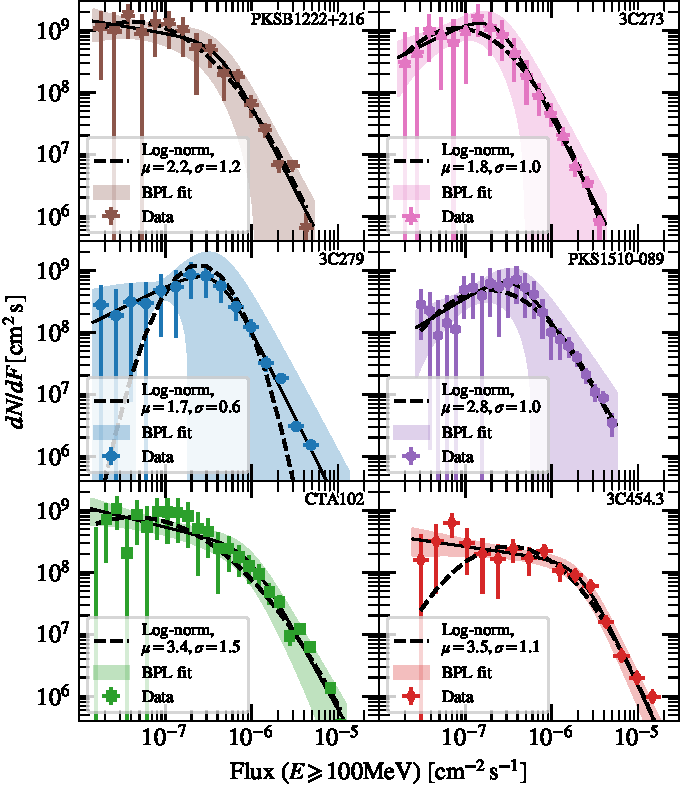
\includegraphics[width = .99\linewidth]{figures/fluxdist_weekly_tsmin9.pdf}
    \caption{\label{fig:fluxpdf} Distribution of the fluxes of the weekly 9.5 year \gray light curves. The BPL fit is shown as a black line with $1\,\sigma$ uncertainties (shaded bands). The black dashed line indicates a fit with a log-normal distribution with location and scale parameters $\mu$ and $\sigma$ as indicated in the legends.}
\end{figure}

\subsection{Determination of the quiescent background level}
\label{sec:qb}
As mentioned in the introduction, 
there is no rigorous way to distinguish the 
flux in flares from the flux 
in a {\em quiescent background} (hereafter QB).
It is not even guaranteed that
there is a corresponding astrophysical distinction.
Nevertheless some progress can be made,
especially given the assumption that the QB is
truly constant.

The minimum flux observed over time 
might be taken as an estimate the true QB,
but it is rather a crude lower limit  -- biased downward 
because of the scatter due to observational errors.
On the other hand, long overlapping tails of flares 
could contribute an approximately constant flux level
yielding an upward bias to some QB estimates.
For the present we assume that overlap of flare tails
is negligible, and propose a statistical
procedure addressing the observational error bias.

This algorithm is based on an approximate 
separation of the distribution function of the observed
fluxes in to two components: 
(a) a low end, and (b) a high end -- dominated by
the QB and the flares respectively.
While not relying on (b) being devoid of any QB flux,
we do assume that (a) contains almost entirely QB flux.
In the picture outlined above, this amounts to the
assumption that the flares are isolated (no overlap) 
and the intervening intervals are essentially pure QB.
The algorithm implements this separation
using only flux values with no regard to 
their time sequence.  It is based on finding the
flux interval that maximizes the symmetry of 
the resulting distribution.


In the following pseudo code, the term distribution
refers to the distribution of low values (a) in a putative
flux interval defining the QB.
\begin{enumerate}
\item Sort the $N$ flux values (with $\mathrm{TS} \geqslant 9)$ in increasing order:
%$F_{n}, n = 1, 2, \dots 
$F_{1} \leqslant F_{2} \leqslant \dots F_{N-1}   \leqslant F_{N} $
\item Define a search grid of flux values $\phi_{m}$, $m = 1,\ldots,M$, 
to serve as candidates for the peak of the distribution. We take these 
values on an evenly spaced grid between the minimum and mean flux $\bar{F}$:
$\phi_m \in [F_1 + \epsilon (\bar{F} - F_1); \bar{F}]$.
By definition the QB is very unlikely to be less than the
minimum flux or exceed the mean.
The factor $\epsilon$ is a small number to  avoid edge effects 
near the generally sparse lower end of the flux distribution.
\item For each $m$ define two intervals  of equal length straddling  $\phi_m$: 
    \begin{itemize}
    \item LOW: from $F_{1}$ to $\phi_m$
    \item HIGH: from $\phi_m$ to $\phi_m + (\phi_m - F_{1})$
    \end{itemize}

\item Construct fine grids of flux values spanning these two intervals
\item Compute the cumulative distributions (CDFs) of the
corresponding flux values 
\item Reverse the  CDF for the HIGH interval 
\item Normalize both CDFs to unity at the peak $\phi_m$
\item Compute the ratio of the posterior probabilities that the CDFs come from different distributions or the same distribution,  using the algorithm of \citet{Wolpert1996}.
\item Find the value of $\phi_m$ that minimizes this ratio, which measures the asymmetry of the total CDF of HIGH and LOW
\item Report the median flux, $F_\mathrm{QB}$, in this
optimally symmetric distribution as the QB estimate
\end{enumerate}
\noindent
%While the CDFs are computed in bins,
In the limit of moderately finely gridded bins 
used in Step 5 the CDF estimate is effectively
unbinned (little or no dependence
on the binning).

We show our estimate for the QB level in Figure~\ref{fig:weekly} as black dashed lines and report the values in Table~\ref{tab:global}.
In general these $F_\mathrm{QB}$ values match 
the visual flux baselines extremely well. 
In the case of 3C454.3, it is slightly higher than the minimum flux level observed for this source around MJD 55800-56200. The reason is our applied $\mathrm{TS}$ cut and a contamination of $F_\mathrm{QB}$ from the tails of the flares. 
We have tested the latter point with simulations drawing random numbers from a uniform distribution and Cauchy distributions to emulate flares. 
For the Cauchy distributions we randomize the height, width, and position. 
Applying our algorithm to these simulated histograms, we find that $F_\mathrm{QB}$ slightly overestimates the true uniform background. Therefore, we conclude that $F_\mathrm{QB}$ can be seen as a firm upper limit on a truly constant QB level. 
We also note that using the peak or mean of the distribution in Step 10, instead of the median,  only changes the results marginally. 
We have furthermore tested different metrics instead of the algorithm of \citet{Wolpert1996}, namely the Kolmogorov-Smirnov (KS) test and the least squares between the CDFs. 
We again find comparable results. However, the KS-test estimates underpredict the true QB level in simulations while the least squares give too high estimates (higher than the Wolpert estimate).
We also note that the $F_\mathrm{QB}$ values are either consistent with or lower than the break flux of the BPL fit, $F_\mathrm{br}$.
This is expected, as $F_\mathrm{QB}$ marks the median of the QB while $F_\mathrm{br}$ probably indicates the transition from the QB to the flaring states. 

\subsection{Determination of the power spectral density}
We further characterize the global \gray light curves in terms of their power spectral density (PSD),
which usually can be described with simple power laws in frequency,  $\mathrm{PSD} \propto 1 / \nu^\beta$.
An analysis of the first 11~months of LAT data from 106 blazars revealed that 
these objects have $\beta$ values between 1 and 2, the intermediate regime between flicker noise ($\beta = 1$) and Brownian motion ($\beta = 2)$~\citep{2010ApJ...722..520A}. 
In addition to the noise behavior, 
we will use the derived PSDs in Section~\ref{sec:gammaradio} to simulate \gray light curves in order to calculate the significance of a correlation between radio and \gray emission. 

The best-fit PSDs are estimated from the periodograms and simulated light curves following the method described in detail in \citet{2014MNRAS.445..437M} and \citet{2013MNRAS.433..907E} and summarized briefly below.
The observed periodograms $P(\nu)$ as a function of frequency (inverse time) $\nu$ are calculated from the absolute square of the Fourier transformation of the light curve (Eq.~3 in \citealt{2014MNRAS.445..437M}). 
We include all data points detected with $\mathrm{TS} \geqslant 9$ and perform a linear interpolation between gaps in the light curve to guarantee an even sampling. 
Since we are using weekly binned light curves and bright FSRQs, the gaps are small and at most 6 consecutive data points long (42\,days) in the case of PKS\,B1222+216. The number of non-detected bins is less than $\sim13\,\%$ for all sources.
The interpolation is done in time steps of $\Delta t=0.7\,$days and 
 the interpolated fluxes are re-binned into bins of lengths of 7 days through averaging.
In contrast to~\citet{2014MNRAS.445..437M}, we do not apply a window function (see the discussion below). 

We compare the observed periodogram with simulated light curves, which we produce with the method of \citet{1995A&A...300..707T} for power-law PSDs with values $0 \leqslant \beta \leqslant 3$ in steps of $\Delta\beta = 0.05$. For each $\beta$ value 100 light curves are generated, each one a 100 times longer than the actual observation to account for possible red-noise leakage. Splitting the simulated light curves (without overlap) leaves us with $10^4$ realizations. 
The light curves are initially produced with a regular time binning equal to 0.7\,days and  re-binned into 7-day light curves through averaging. 
The same observational gaps and interpolation as in the observed light curves are applied. 
The periodograms are then calculated for the simulated light curve in the same way as for the observed one.

To fix the normalization of the PSD model, \citet{2014MNRAS.445..437M} suggest variance matching, i.e., they rescale the simulated flux data points with a factor $A^{-1}$, where $A^2 = \sigma_\mathrm{sim}^2 / (\sigma_\mathrm{obs}^2 - \bar{\sigma_i^2})$, with $\sigma_\mathrm{sim}^2$ ($\sigma_\mathrm{data}^2$) the variance of the simulated (observed) light curve and $\bar{\sigma_i^2}$ the variance of the observational noise.
For the \gray light curves, we choose to follow \citet{2013MNRAS.433..907E} instead and iteratively match the probability distribution of the simulated fluxes to the observed ones, given by the $dN/dF$ distributions shown in Figure~\ref{fig:fluxpdf}. 
The reason is that the algorithm of \citet{1995A&A...300..707T} produces light curves with Gaussian distributed fluxes, which is clearly not the case at \gray energies.\footnote{Furthermore, the variance matching relies on Parseval's theorem from which it follows that the light curve variance is equal to the integrated PSD. However, Parseval's theorem is only valid for square-integrable functions, i.e. $\beta \geqslant 2$ and thus not strictly applicable for smaller values of $\beta$ commonly observed at \gray energies.}
In a final step, we add uncertainties to the light curves by randomly drawing with replacement from the observed uncertainties $\sigma_i$ and adding a Gaussian random number $\mathcal{N}(0,\sigma_i)$ to the simulated flux values.

The peridograms of the observed and simulated light curves, ${P}_\mathrm{obs}$ and ${P}_\mathrm{sim}$, are averaged in logarithmic bins~\citep{1993MNRAS.261..612P} and compared by means of a $\chi^2$ test~\citep{2014MNRAS.445..437M},
\begin{equation}
    \chi^2(\beta) = \sum_{\nu_\mathrm{min}}^{\nu_\mathrm{max}}\frac{(P_\mathrm{obs}(\nu) - \overline{P}_\mathrm{sim}(\nu,\beta))^2}{\Delta\overline{P}_\mathrm{sim}(\nu,\beta)^2},\label{eq:chi2psd}
\end{equation}
where $\overline{P}_\mathrm{sim}(\nu)$ and $\Delta\overline{P}_\mathrm{sim}(\nu)^2$ are the mean and variance of the periodograms obtained from the simulated light curves.
The averaged periodograms of the simulated light curves and the observed ones are shown in Figure~\ref{fig:periodograms} and the best-fit average periodogram is shown as a thick solid line. 
The quality of the the best-fit value $\hat\beta$ with corresponding minimum $\chi^2$ value $\hat\chi^2\equiv\chi^2(\hat\beta)$, is evaluated from the light curves simulated with $\beta = \hat\beta$ in the following way. We form the distributions of simulated $\chi^2$ values, $\chi^2_\mathrm{sim}$, by replacing $P_\mathrm{obs}(\nu)$ with $P_\mathrm{sim}(\nu,\beta)$ in Eq.~(\ref{eq:chi2psd}),
\begin{equation}
    \chi^2_\mathrm{sim}(\beta,\beta') = \sum_{\nu_\mathrm{min}}^{\nu_\mathrm{max}}\frac{(P_\mathrm{sim}(\nu,\beta) - \overline{P}_\mathrm{sim}(\nu,\beta'))^2}{\Delta\overline{P}_\mathrm{sim}(\nu,\beta')^2},\label{eq:chi2psd_sim}
\end{equation}
and calculate the $p$-value, $p_\beta$, as the  fraction of simulations that result in $\chi^2_\mathrm{sim}(\hat\beta,\hat\beta) > \hat\chi^2$.\footnote{From the $10^4$ simulations we effectively derive a histogram of the $10^4$ $\chi^2_\mathrm{sim}(\hat\beta,\hat\beta)$ values from which we then determine $p_\beta$.}
The confidence interval for $\hat\beta$ is derived by determining the $\Delta\chi^2_\mathrm{sim}(\hat{\beta},\beta)$ value from simulations such that 95\,\% of the time the simulated (true) $\beta$ value is contained within $\Delta\chi^2$.\footnote{Put differently, the $10^4$ simulated light curves provide $10^4$ $\chi^2$ curves as functions of $\beta$ from which we calculate the value of $\Delta\chi^2$ such that the true (simulation-input) $\beta$ value is contained within that interval in 95\,\% of the times.}
The same $\Delta\chi^2$ value is then applied to the observed $\chi^2$ curve.
The results of our PSD analysis are summarized in Table~\ref{tab:global} where we also report the value of $\beta$ obtained from a linear regression in log-log space. 
In general, the periodograms are well fit by our method, as indicated by the $p_\beta$-values and observed in Figure~\ref{fig:periodograms}. 
The only exception is 3C279 where only 2 of the $10^4$ simulated light curves result in a $\chi^2_\mathrm{sim}(\hat\beta,\hat\beta) > \hat\chi^2$.
The steep $\chi^2$ curve for this source also explains the small error bars on the reconstructed value of $\beta$.
The reason might be a more complex underlying PSD or the specific 7 day binning we have chosen here. 
\begin{figure*}
    \centering
    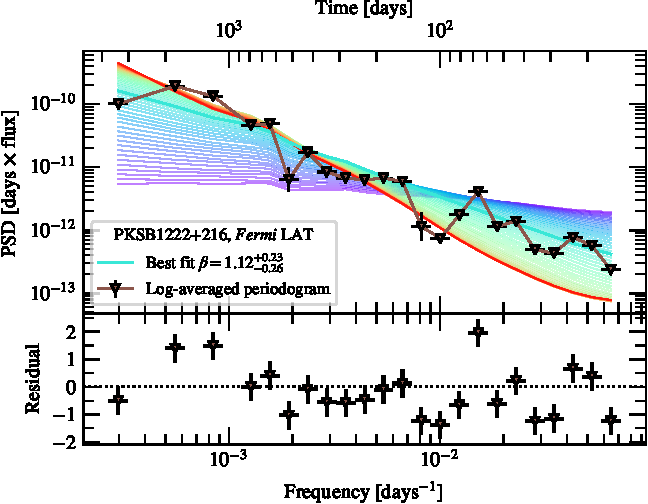
\includegraphics[width = 0.32\linewidth]{figures/periodogram_fermi_PKSB1222+216_Nsim_100Next_100Sim_addunc_data_rescale_EM13_usegap_1_PSD_window_none_detrend_none_norm_var_20.pdf}
    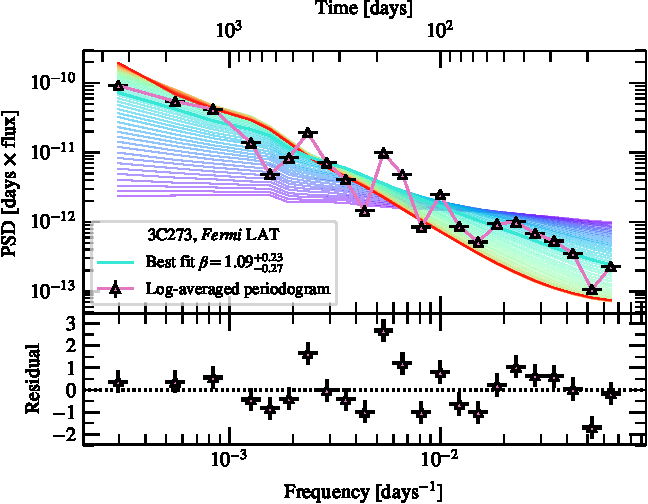
\includegraphics[width = 0.32\linewidth]{figures/periodogram_fermi_3C273_Nsim_100Next_100Sim_addunc_data_rescale_EM13_usegap_1_PSD_window_none_detrend_none_norm_var_20.pdf}
    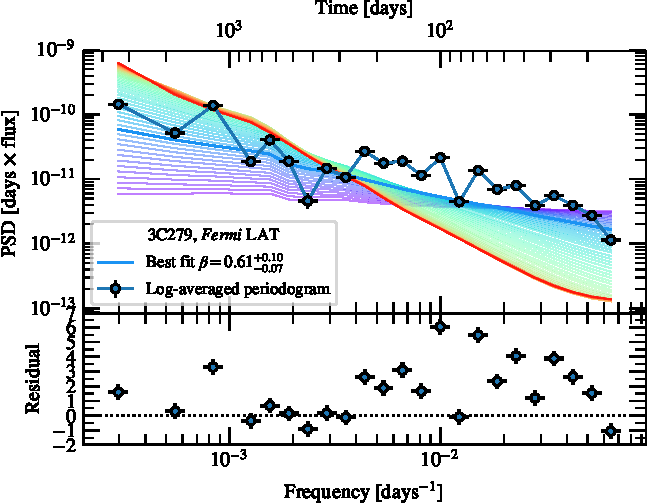
\includegraphics[width = 0.32\linewidth]{figures/periodogram_fermi_3C279_Nsim_100Next_100Sim_addunc_data_rescale_EM13_usegap_1_PSD_window_none_detrend_none_norm_var_20.pdf}
    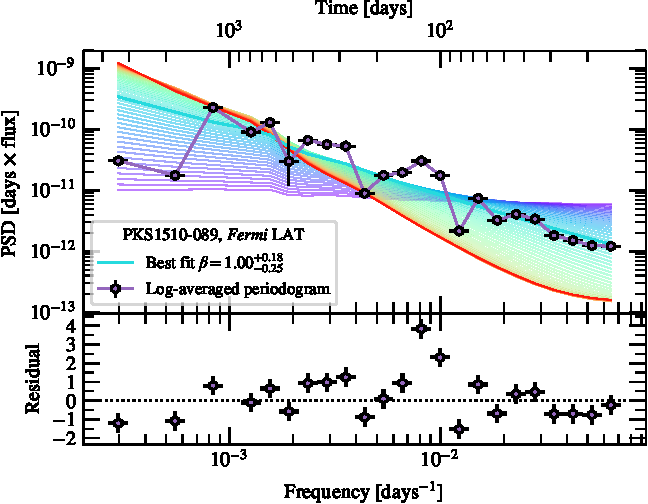
\includegraphics[width = 0.32\linewidth]{figures/periodogram_fermi_PKS1510-089_Nsim_100Next_100Sim_addunc_data_rescale_EM13_usegap_1_PSD_window_none_detrend_none_norm_var_20.pdf}
    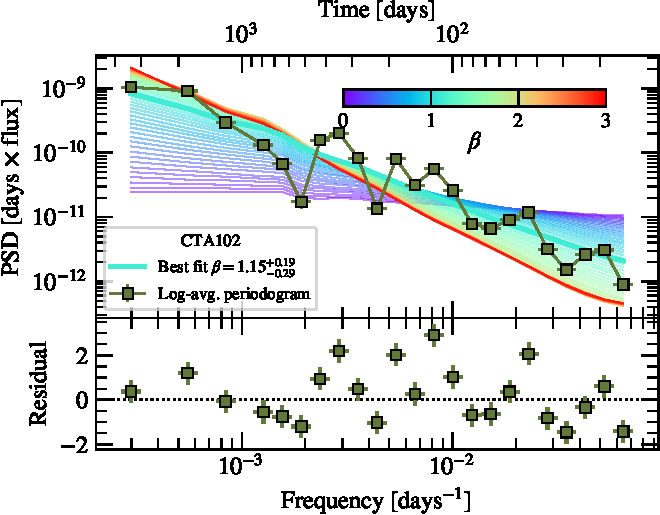
\includegraphics[width = 0.32\linewidth]{figures/periodogram_fermi_CTA102_Nsim_100Next_100Sim_addunc_data_rescale_EM13_usegap_1_PSD_window_none_detrend_none_norm_var_20.pdf}
    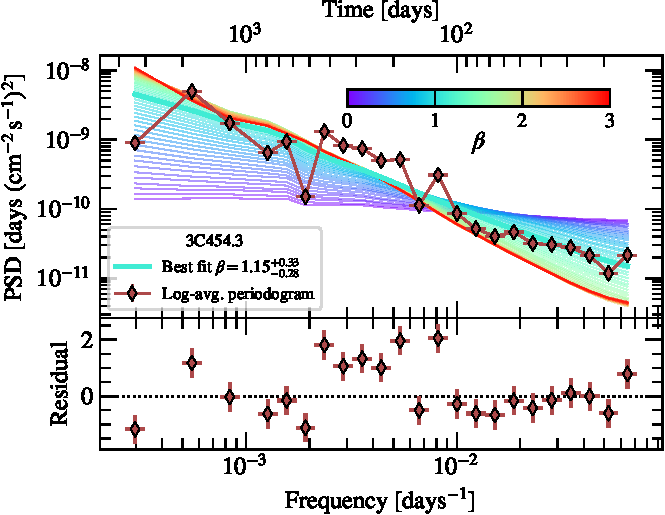
\includegraphics[width = 0.32\linewidth]{figures/periodogram_fermi_3C454p3_Nsim_100Next_100Sim_addunc_data_rescale_EM13_usegap_1_PSD_window_none_detrend_none_norm_var_20.pdf}
    \caption{Periodograms of the observed (markers) and simulated light curves (colored lines). The simulated periodograms follow power-law PSDs between $\beta = 0$ (purple line) to $\beta = 3$ (red line) in steps of $\Delta\beta = 0.05$. The bottom panels show the residuals with respect to the best fit which is indicated in the legend and as a thick solid line in the upper panels.}
    \label{fig:periodograms}
\end{figure*}


\begin{deluxetable*}{l|ccc|c|ccc}
\tablewidth{0pt}
\tablecaption{ \label{tab:global}Global \gray light curve properties.}
\tablehead{\colhead{Source name} & 
\colhead{$\alpha_\mathrm{low}$} &
\colhead{$\alpha_\mathrm{high}$} & 
\colhead{$F_\mathrm{br} [10^{-6}\mathrm{cm}^{-2}\mathrm{s}^{-1}]$} &
\colhead{$F_\mathrm{QB} [10^{-7}\mathrm{cm}^{-2}\mathrm{s}^{-1}]$} &
\colhead{$\beta_\mathrm{slope}$} &
\colhead{$\hat\beta$} &
\colhead{$p_\beta$}
}
\startdata
PKSB1222+216 & $-0.24^{+0.41}_{-0.27}$ & $-2.70^{+0.33}_{-0.43}$ & $0.42^{+0.28}_{-0.15}$ & 1.49 & 1.23 & $1.12^{+0.21}_{-0.26}$ & 0.423 \\
3C273 & $0.70^{+0.40}_{-0.54}$ & $-2.77^{+0.24}_{-0.27}$ & $0.23^{+0.07}_{-0.07}$  & 1.87 & 1.14 & $1.09^{+0.24}_{-0.27}$ & 0.330 \\
3C279 & $0.68^{+0.27}_{-0.40}$ & $-2.80^{+0.21}_{-0.23}$ & $0.40^{+0.10}_{-0.10}$ & 3.23 & 0.67 & $0.61^{+0.10}_{-0.07}$ & $2\times10^{-4}$ \\
PKS1510-089 & $0.84^{+0.72}_{-0.48}$ & $-2.21^{+0.23}_{-0.26}$ & $0.40^{+0.16}_{0.12}$ & 4.19 & 0.88 & $1.00^{+0.18}_{-0.25}$ & 0.129 \\
CTA102 & $-0.35^{+0.22}_{-0.18}$ & $-2.50^{+0.16}_{-0.19}$ & $0.90^{+0.38}_{-0.26}$ & 2.49 & 1.21 & $1.18^{+0.16}_{-0.32}$ & 0.138 \\
3C454.3 & $-0.20^{+0.17}_{-0.13}$ & $-3.00^{+0.13}_{-0.14}$ & $2.19^{+0.39}_{-0.32}$ & 8.59 & 1.05 & $1.15^{+0.32}_{-0.28}$ & 0.274 \\
\enddata
{
\tablecomments{Columns 2-4 indicate the best-fit values for the BPL fit [Eq.~(\ref{eq:dndf})] to the $dN/dF$ distributions, column 5 reports our estimate of the QB flux, and columns 6-8 show the best-fit results for the PSD. $\beta_\mathrm{slope}$ gives the result for a linear regression of the periodograms and $\hat\beta$ is the best-fit value of the $\chi^2$ minimization with corresponding $p_\beta$-value. The interval around $\hat\beta$ is at 95\,\% confidence.}
}
\end{deluxetable*}

\section{Results for local light curve properties}
\label{sec:results-local}
%\subsection{Local light curve properties}
%\label{sec:hop-fit}

We proceed with deriving local properties of the \gray flares, focusing first on the light curves with one bin per GTI that are shown in Figure~\ref{fig:gti}.
The average best-fit spectral parameters for the entire time spans of the daily, orbital, and sub-orbital light curves (the time ranges for the sub-orbital light curves are indicated as solid horizontal bars in Figure~\ref{fig:gti}) are summarized in Table~\ref{tab:avg-spec} in Appendix~\ref{sec:avg-spec}. 

%%% GTI light curves %%%%%%%%%
\begin{figure*}
    \centering
    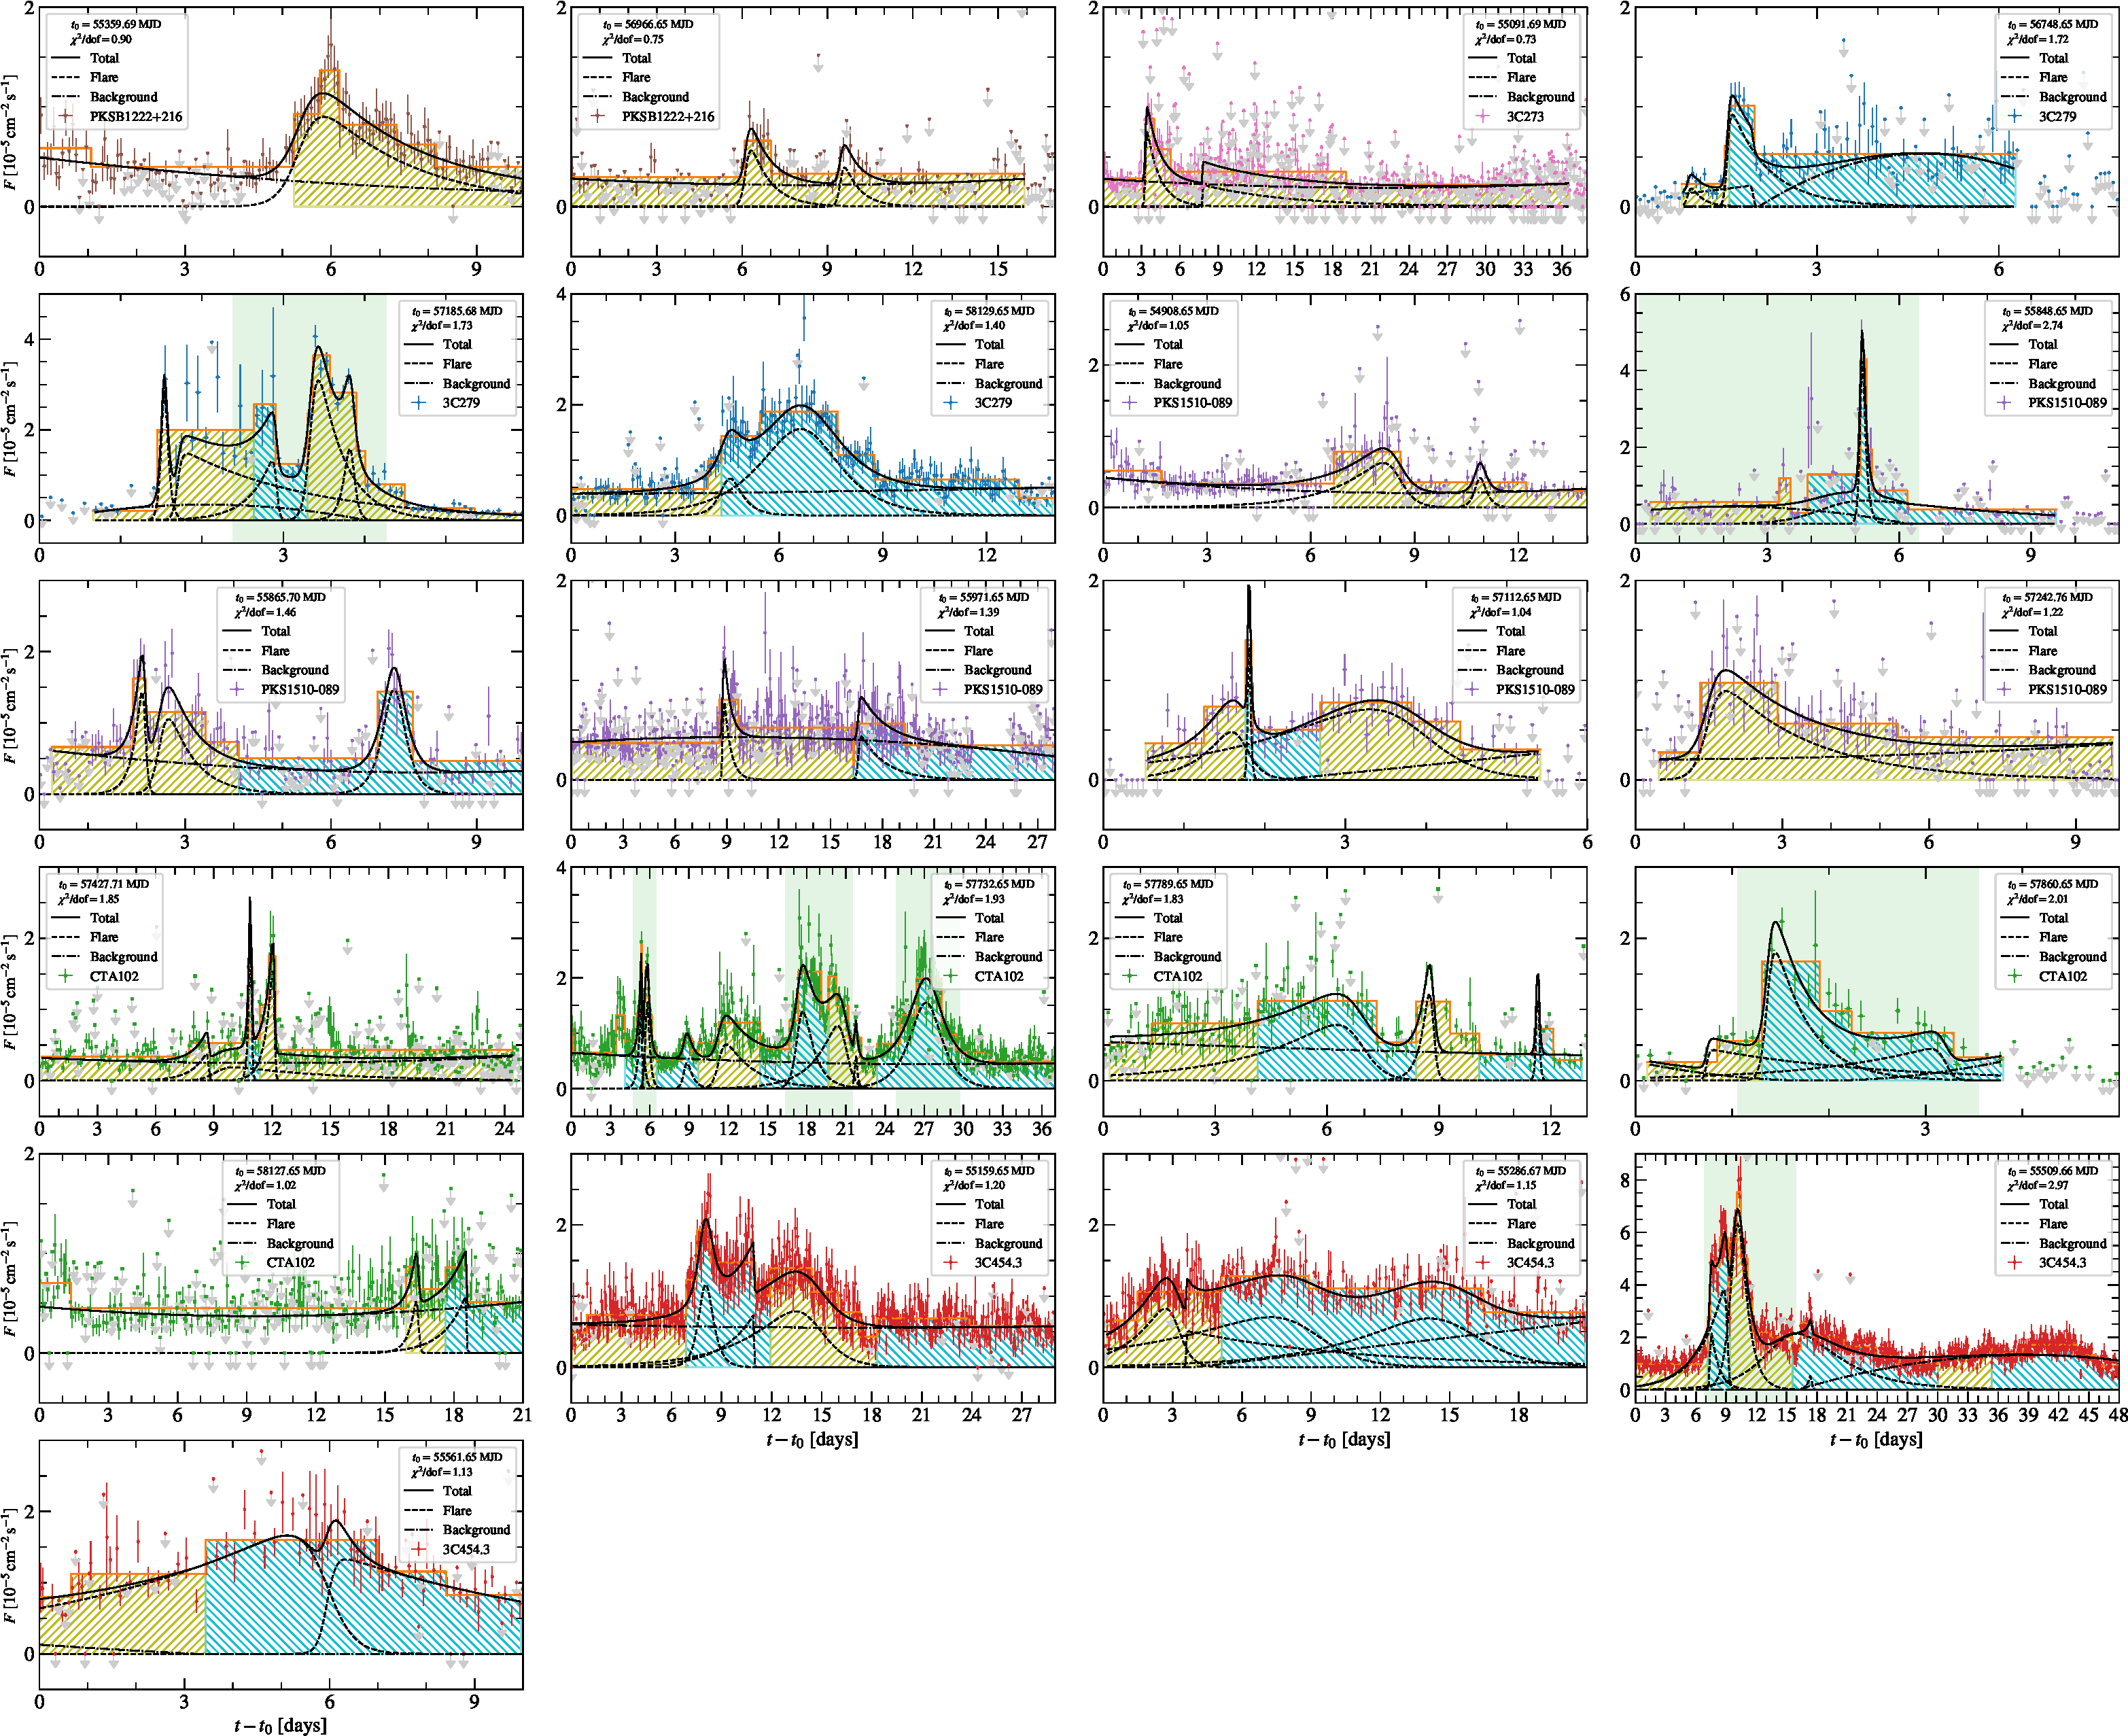
\includegraphics[width = .99\linewidth]{figures/lcfithop_orbit_all_maxiter2_fsys0p00_addcomp0_comb.pdf}
    \caption{ Light curves with one bin per GTI for the selected time ranges (solid horizontal lines in Figure~\ref{fig:daily}). Solid black and dashed lines show fits to the light curve with exponential flare profiles discussed in Section~\ref{sec:results-local}. Other symbols and lines are the same as in Figure~\ref{fig:weekly} and ~\ref{fig:daily}.
    The sub-GTI light curves are derived for the time intervals indicated as solid horizontal lines, where at least one orbital bin shows $\mathrm{TS}\geqslant 150$ (see Section~\ref{sec:sub-gti}). 
    Average spectra to search for a cut-off due to \gray absorption in the BLR are derived from the time intervals indicated either as solid or dashed horizontal lines (see Section~\ref{sec:blrabs}).
    }
    \label{fig:gti}
\end{figure*}
%%%%%%%%%%%%%%%%%%%%%%%%%%%%%%

We again use BBs and HOP groups to identify different states in 
the orbital light curves (orange lines and hatched regions in Figure~\ref{fig:gti}). 
To assess the time profile of the flares,
we fit each HOP group $i$ with a sum of exponential profiles, $F_{\mathrm{flare},i}$,
using a $\chi^2$ minimization, and
\begin{eqnarray}
    F_{\mathrm{flare},i}(t) &=& 
    \sum\limits_{j = 1}^{N_i} F_{0,ij}\nonumber\\
    &\times&\left[\exp\left(\frac{t - t_{0,ij}}{\tau_{\mathrm{rise},ij}}\right) + \exp
    \left(\frac{t_{0,ij} - t}{\tau_{\mathrm{decay},ij}}\right)\right]^{-1}\!\!\!,
    \label{eq:flareHOP}
\end{eqnarray}
where $t_{0,ij}$ are the times when the flare flux is equal to $F_{0,ij} / 2$, and $\tau_{\mathrm{rise},ij}$, $\tau_{\mathrm{decay},ij}$ are the flare rise and decay times, respectively.
All light curve points are included that fulfill $\mathrm{TS}\geqslant9$ and $F_i \geqslant 3\sigma_i/2 $.
The number of flare profiles per HOP group, $N_i$, is either 1 or 2 and determined during the fit using the Bayesian information criterion (BIC), defined as $\mathrm{BIC} = n_\mathrm{par}\ln(n) + \chi^2$, where $n_\mathrm{par}$ is the number of fit parameters ($n_\mathrm{par} = 4$ for $N_i = 1$), and $n$ is the number of data points within one HOP group $i$. 
Two flare profiles are selected if the difference between the two BIC values is $\Delta\mathrm{BIC} = \mathrm{BIC}(N_i = 2) - \mathrm{BIC}(N_i = 1) < 0$.
The reason for allowing $N_i > 1$ is that the flare profile in Eq.~\ref{eq:flareHOP} does not capture long-lasting plateaus of a flare (see, e.g., all flares of 3C279 or the last panel with the flare of 3C454.3 starting at 55551.65\,MJD in Figure~\ref{fig:gti}).

After each HOP group is fitted individually and $N_i$ is determined, 
we re-fit the entire light curve, which consists of $N_\mathrm{HOP}$ groups, with the function 
\begin{equation}
    F_\mathrm{flare}(t) = \sum\limits_{i = 1}^{N_\mathrm{HOP}}F_{\mathrm{flare},i}(t) + F_\mathrm{bkg}(t),
\end{equation}
where $F_\mathrm{bkg}(t)$ is an order-2 polynomial to describe a slow  varying background.
The fit results are shown as black solid lines in Figure~\ref{fig:gti}.
In general, the $\chi^2$ values divided by the degrees of freedom (dof) are between 1 and 2 (see the legends in Figure~\ref{fig:gti}). Given the large values of dof, the fit qualities are generally poor. This is not unexpected, as we only allow up to two flare profiles per HOP group and not arbitrary functions. Already with this choice, there are probably some spurious flares identified, see, e.g., the second flare profile in the first PKS\,1510-089 flare (starting at 54908.65MJD). 
Nevertheless, the overall light curve evolution is well captured, which allows us to describe the local flare properties from the ensembles of flare profiles. %, keeping the above caveats in mind. 

%We show the distribution of rise and decay times in the histograms of Figure~\ref{fig:times-hist} for flares with a time-integrated flux $>10^{-7}\,\mathrm{cm}^{-2}$. 
We show the distribution of rise and decay times in  Figure~\ref{fig:times-hist} for flares with a time-integrated flux $>10^{-7}\,\mathrm{cm}^{-2}$. 
Remarkably, all sources show values of $\tau_\mathrm{rise}$ and $\tau_\mathrm{decay}$ that are close or below the horizon crossing time scale of the central super massive black hole,
$t_g = r_g / c$, with $r_g = 2 G M_\bullet / c^2 $ the gravitational radius, $G$ the gravitational constant, black hole mass $M_\bullet$ (taken from Table~\ref{tab:src-select}), and $c$ the speed of light.
This results in values between $\sim0.5$ and $\sim2.5$ hours using the black hole masses listed in Table~\ref{tab:src-select}.

\begin{figure}
    \centering
%    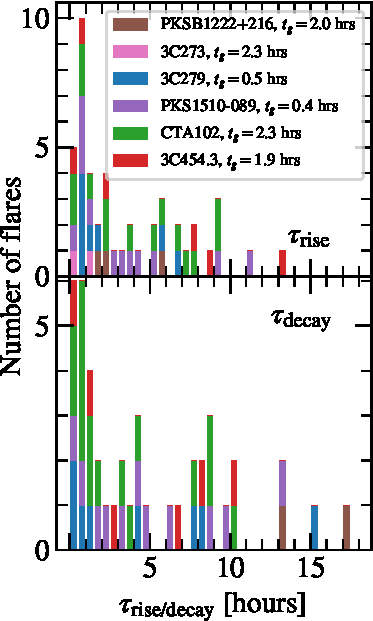
\includegraphics[width = .7\linewidth]{figures/lcfithop_results_tdtrhist_maxiter2_fsys0p00_addcomp0_orbit.pdf}
    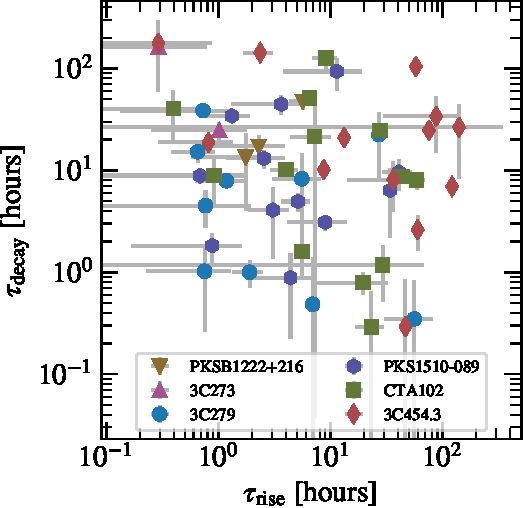
\includegraphics[width = .9\linewidth]{figures/lcfithop_results_trise_vs_tdecay_orbit_maxiter2_fsys0p00_addcomp0.pdf}
    \caption{
    %Stacked bar graphs for  rise (top) and decay times (bottom) for the individual flares fitted in Figure~\ref{fig:gti}. The legend gives the horizon crossing time scales $t_g$ in the observer's frame.
    Distribution of rise and decay times for the flare profiles fitted to data. 
    }
    \label{fig:times-hist}
\end{figure}

From the rise and decay times, we can calculate the flare asymmetry as
\begin{equation}
    A = \frac{\tau_\mathrm{rise}-\tau_\mathrm{decay}}
    {\tau_\mathrm{rise}+\tau_\mathrm{decay}},
\end{equation}
so that $A < 0$ for fast-rise-exponential-decay (FRED) type flares, as expected from an injection of energetic particles that subsequently cool through radiative processes such as inverse Compton scattering or synchrotron emission.
The asymmetry is shown versus integrated flux, peak flux, and flare duration $T_{90}$, defined as the time around the flare peak that contains 90\,\% of the integrated flux, in Figure~\ref{fig:asym}.
The peak flux for each flare of each HOP group is derived from the maximum of  Eq.~\ref{eq:flareHOP} with respect to time (suppressing indices $ij$),

\begin{equation}
    F_{\mathrm{peak}} = \frac{F_{0} \tau_\mathrm{rise}}{\tau_\mathrm{rise} + \tau_\mathrm{decay}}\exp\left(\ln\left(\frac{\tau_\mathrm{decay}}{\tau_\mathrm{rise}}\right)\frac{\tau_\mathrm{decay}}{\tau_\mathrm{rise} + \tau_\mathrm{decay}}\right).
\end{equation}
The error bars on the peak flux and asymmetry are derived from standard Gaussian error propagation from the fit uncertainties.

\begin{figure*}
    \centering
    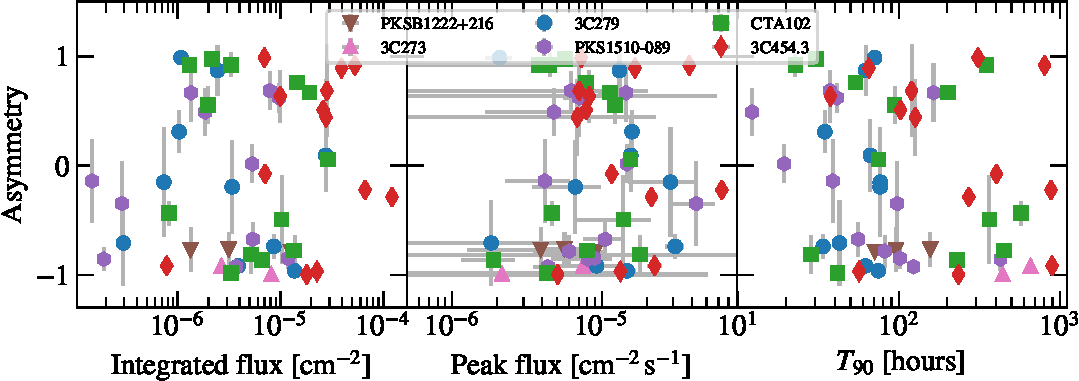
\includegraphics[width = .8\linewidth]{figures/lcfithop_results_asym_vs_all_orbit_maxiter2_fsys0p00_addcomp0.pdf}
    \caption{Flare asymmetry versus integrated flux (left), peak flux (center), and flare duration $T_{90}$ (right) for the fitted flare profiles shown in Figure~\ref{fig:gti}.}
    \label{fig:asym}
\end{figure*}

The median of the asymmetry is found to be $-0.195$, i.e., FRED-type flares are more common than the opposite. In general, the flares show a versatile behaviour and no clear trends are seen from Figure~\ref{fig:asym}. This is also reflected in the fact that we do not find any significant correlation between the asymmetry, integrated and peak flux, rise and decay times, as well as flare duration using Kendall's $\tau$.

We also investigate whether subsequent flares in each panel of Figure~\ref{fig:gti} show a trend with time in peak flux, asymmetry, or duration. 
For consecutive flares, we calculate the difference between, e.g., the peak fluxes, and calculate the $p$-value of a binomial distribution assuming an equal probability of finding negative and positive differences.
For 32 values of differences the $p$-values for the peak flux, asymmetry, as well as for the flare duration are close to 0.1 (14, 13, and 13 positive values for 32 trials, respectively) indicating no particular evolution of these quantities with time. 

We also find complex behavior of the spectral evolution during the flares. Evidence for a  ``harder-when-brighter'' trend is found for some sources and flares, which is however not significant. 
We therefore cannot draw any firm conclusions from the spectral evolution, which we show for reference in Figure~\ref{fig:specvar} in  Appendix~\ref{sec:specvar}. 



\subsection{Sub-GTI light curves}
\label{sec:sub-gti}
We search for sub-orbital variability in a subset of orbital light curves, namely in those where at least one orbital bin is detected with $\mathrm{TS} \geqslant 150$. 
In this way we ensure high photon statistics and reduce the number of trials when searching for minute scale variability (for comparison, the orbital light curve bin for which \citet{TheFermi-LAT:2016dss} measured minute scale variability in 3C279 is detected in our analysis with $\mathrm{TS} \sim 400$). 
The selected time regions are indicated with solid horizontal lines regions in Figure~\ref{fig:gti}, whereas the dashed lines show the time intervals selected with the criteria in Table~\ref{tab:zoom} that do not pass the additional $\mathrm{TS}$ cut.

The resulting light curves, binned such that the uncertainty in each bin is of the order of $\sim20\,\%$ \citep[using the adaptive binning introduced by][]{lott2012}, are shown in Figure~\ref{fig:lc_minutes}. 
In order to make an objective selection of GTIs that we test against the hypothesis of a constant flux, we consider only those where the BBs indicate a significant flux change within the GTI (GTIs marked in green in Figure~\ref{fig:lc_minutes}).
Naively, one could expect that a BB change within one GTI would correspond to a significance of 95\,\% for a non-constant flux, since this is the threshold we have selected in the BB algorithm~\citep{2013ApJ...764..167S}. However, the BB algorithm also takes data before and after the particular GTI into account and only provides qualitative evidence for minute-scale variability. 
Therefore, we test each bin selected in this way against the hypothesis of constant flux, using a simple $\chi^2$ test. 
The best-fit constant flux is given by $\hat{F} = (\sum (F_i / \sigma_i^2))(\sum F_i^{-2})^{-1}$. 
For the GTIs where the constant fit results in a pre-trial $p$-value of less than 0.1, we show the sub-GTI light curves in Figure~\ref{fig:singel-gtis} and report the pre- and post-trial fit probabilities in Table~\ref{tab:minute}.
We count each tested GTI as one trial. 
We also provide the minimum values for the variability times for pairs of fluxes $F_i$ and $F_j$ measured at $t_i$ and $t_j$, respectively, given by~\citet{1999ApJ...527..719Z},
\begin{equation}
t_{\mathrm{var},ij} = \frac{F_i + F_j}{2}\left|\frac{t_i - t_j}{F_i - F_j}\right|.
\end{equation}
The pre-trial $p$-values for rejecting the constant-flux hypothesis are all around $2\,\sigma$. 
The trial correction leaves only one GTI of 3C279 and two GTIs for CTA102 close to or above a $2\,\sigma$ evidence for a variable flux. 
However, inspecting the light curve the second GTI of CTA102 (starting at MJD\,57758.86, see Figure~\ref{fig:singel-gtis}), the high $\chi^2$ value might be the result of our chosen binning; the first bin actually spans a long time range for which the exposure is mostly zero.  
For the other two GTIs the suggested variability times scales are between 3 and 4\,minutes.

In comparison to previous results for 3C279 and CTA102, our method results in lower significance detections of minute-scale variability.
In comparison to~\citet{2018ApJ...854L..26S}, we also find evidence for minute scale variability in different GTIs. 
This is due to trial correction but probably also due to differences in the analysis.
For example, we use a finer binning for the exposure in the azimuthal direction to take this dependence for such short observations into account.
The change in exposure is, however, below 10\,\%.
More importantly, we use a different binning within one GTI, which can also change the significance. 
Taking the $\chi^2$ test and the BBs together, we conclcude that we find evidence that minute-scale variability is common phenomenon during bright FSRQ flares. %we find weak evidence for minute-scale variability for 3C454.3 and PKS1510-089 and stronger evidence for 3C279 and CTA102.
\begin{figure*}
    \centering
    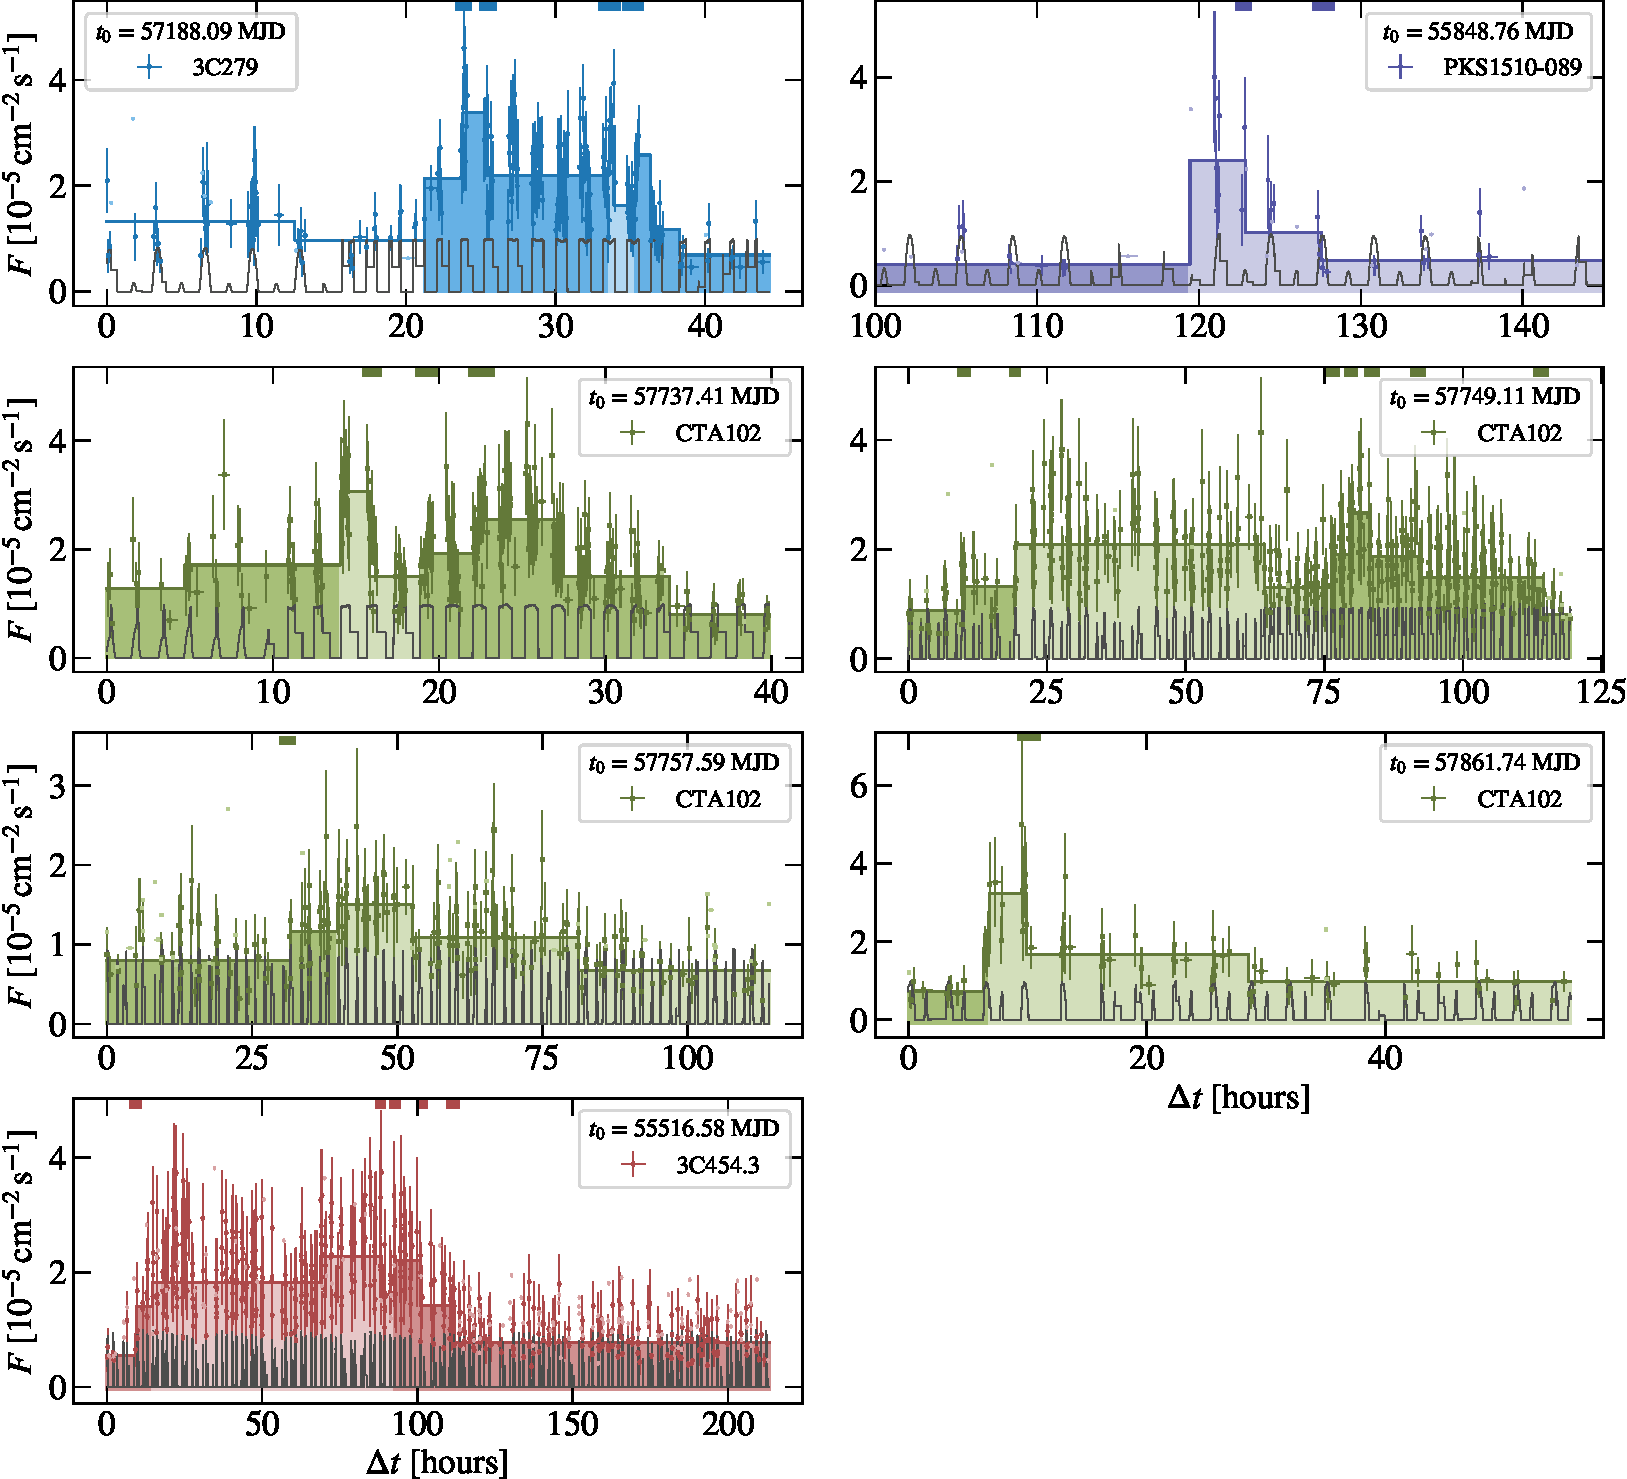
\includegraphics[width = .9\linewidth]{figures/lc_minute_3min.pdf}
    \caption{Sub-GTI light curves for the HOP groups of the orbital light curves which contain one bin with $\mathrm{TS} \geqslant 150$. The solid horizontal lines indicate GTIs that encompass a significant flux change found by the BB algorithm. The dark grey curves show the relative exposure at 1\,GeV. The ToO campaigns for 3C279 (upper left panel) and CTA102 (upper right panel) are clearly visible as the exposure is constant over several GTIs. }
    \label{fig:lc_minutes}
\end{figure*}

\begin{figure*}
\centering
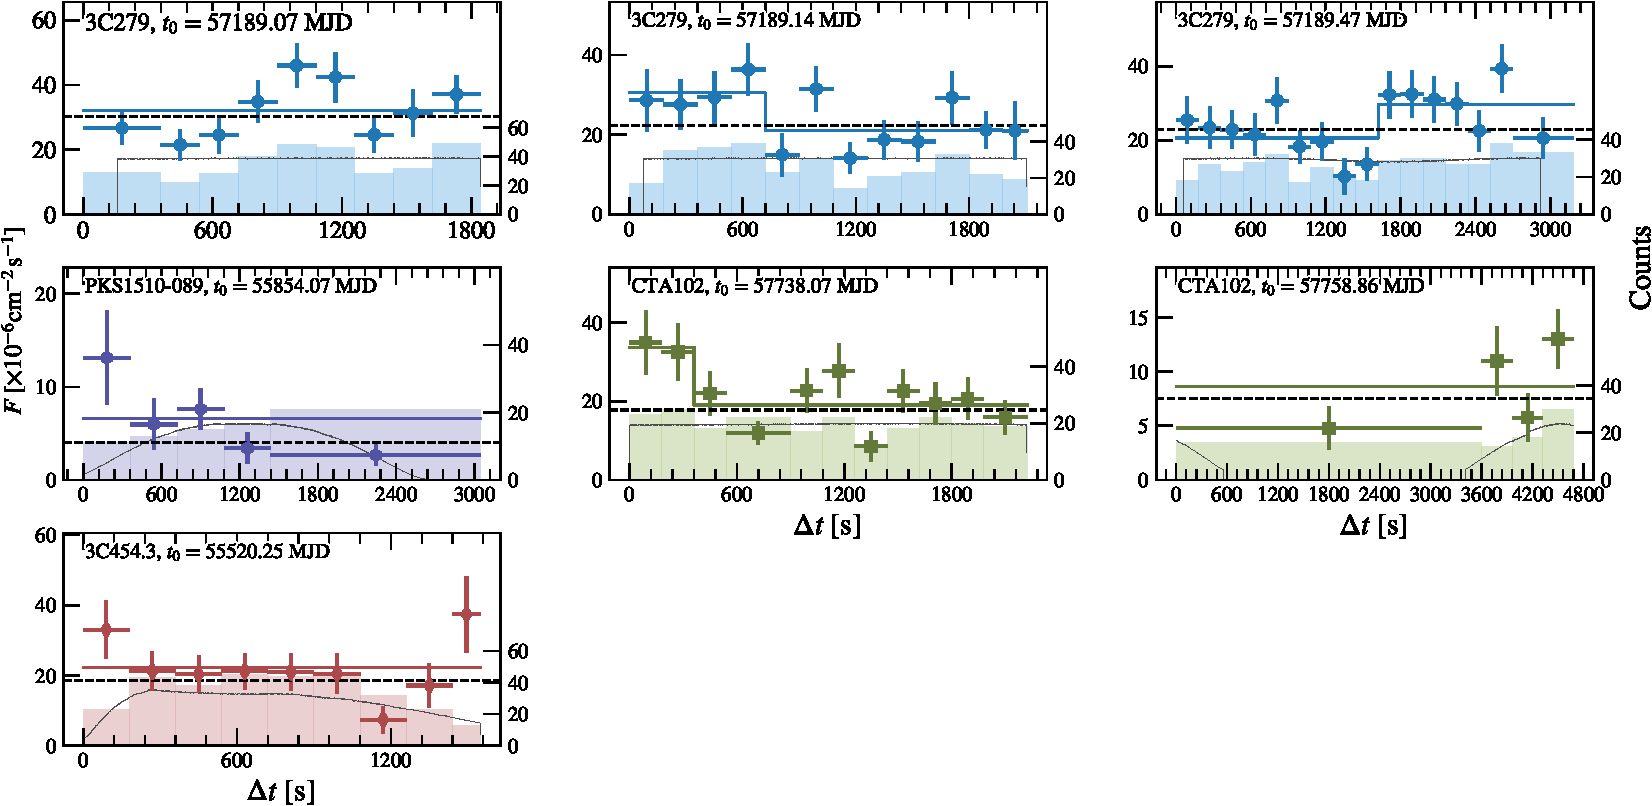
\includegraphics[width = .95\linewidth]{figures/minute_lc_adaptive20.pdf}
\caption{Light curves of single GTIs for which the BBs for the full time interval indicate a flux change within the GTI (solid horizontal lines in Figure~\ref{fig:lc_minutes}) and for which a fit with a constant flux results in a fit significance of less than 0.1. The orange lines indicate BBs if only the data within the GTI is taken into account. The black dashed line is the best-fit value of the constant flux. The grey histograms show the number of counts in each bin and the dark grey lines indicate the relative source exposure as a function of time. }
\label{fig:singel-gtis}
\end{figure*}

\begin{deluxetable}{cccccc}
\tablewidth{0pt}
\tabletypesize{\scriptsize}
\tablecaption{ \label{tab:minute}Results from sub-GTI light curves on minutes-scale variability.}
\tablehead{\colhead{$t_0$} & \colhead{$\Delta t$}  & \colhead{$\chi^2 / \mathrm{d.o.f.}$} & \colhead{$p$-value} & \colhead{$p$-value}& \colhead{$\mathrm{min}(t_\mathrm{var})$}  \\ 
{} [MJD] & [mins] & {} & (pre trial) & (post trial) & [mins]}
\startdata
\hline
\multicolumn{6}{c}{3C279}\\
\hline
57189.07 & 30.72 & 1.93 & 0.051 (1.95$\sigma$) & 0.188 (1.32$\sigma$) & $5.6\pm2.8$ \\
57189.14 & 35.13 & 1.68 & 0.071 (1.81$\sigma$) & 0.254 (1.14$\sigma$) & $3.6\pm1.4$ \\
57189.47 & 53.08 & 1.94 & 0.015 (2.42$\sigma$) & 0.060 (1.88$\sigma$) & $3.7\pm1.4$ \\
\hline
\multicolumn{6}{c}{PKS1510-089}\\
\hline
55854.07 & 50.80 & 2.01 & 0.091 (1.69$\sigma$) & 0.173 (1.36$\sigma$) & $7.9\pm5.0$ \\
\hline
\multicolumn{6}{c}{CTA102}\\
\hline
57738.07 & 37.04 & 2.30 & 0.011 (2.55$\sigma$) & 0.032 (2.14$\sigma$) & $2.8\pm1.0$ \\
57758.86 & 78.00 & 2.62 & 0.049 (1.97$\sigma$) & 0.049 (1.97$\sigma$) & $7.8\pm3.7$ \\
\hline
\multicolumn{6}{c}{3C454.3}\\
\hline
55520.25 & 25.83 & 1.96 & 0.048 (1.98$\sigma$) & 0.216 (1.24$\sigma$) & $3.2\pm1.6$ \\
\enddata
{
\tablecomments{The number of trials is counted for each flare individually and given by the number of horizontal solid lines in each panel of Figure~\ref{fig:lc_minutes}.}
}
\end{deluxetable}


\section{Location of the $\gamma$-ray emitting region}
\label{sec:location}

The location of the \gray emission region in blazar jets remains unknown. 
From the rich data set of the six FSRQs studied here, we attempt to constrain the position of the emitting region using three independent approaches. 
First, in Section~\ref{sec:blrabs}, we search for absorption signatures in the LAT spectra caused by pair production of \Grays with photons of external photon fields. We use spectra during the brightest flares identified in the orbital light curves in Figure~\ref{fig:gti} (dashed and solid horizontal bars).
The derived constraints on the position are used to calculate energy dependent cooling times in Section~\ref{sec:tcool}, which will be compared against our results for the decay times for the whole energy range (see Section~\ref{sec:results-local}) and for energy dependent light curves.
As shown by~\citet{2012ApJ...758L..15D}, if the flux decay is dominated by radiative cooling in external radiation fields, the energy dependence of the decay times can be used to distinguish inverse-Compton cooling in the radiation fields of the BLR or the dust torus.
This provides additional information about the position of the \gray emission region.
In Section~\ref{sec:gammaradio}, we search for time lags between \gray and radio emission. 
In the scenario where the non-thermal emission is triggered by, e.g., shocks propagating downstream through the jet, a time lag can be translated into the spatial separation between the radio and \gray emitting regions~\citep{2014MNRAS.445..428M}. 
With information about the location of the radio core, the position of the \gray emitting region can be constrained~\citep[e.g.,][]{2014MNRAS.441.1899F}. 

\subsection{Results from spectral fits to \gray data}
\label{sec:blrabs}
\subsubsection{\gray attenuation}
The attenuation due to pair production on a radiation field of soft photons should manifest itself as a cut-off feature in the \gray spectrum. 
The cut-off energy depends on the distance of the \gray emitting region to the central black hole, $r$, and the photon density of the considered photon field.
For FSRQs, photon densities of external radiation fields of the accretion disk, the BLR, and the extended dust torus usually dominate those of internal synchrotron emission~\citep[see,e.g.,][]{2012ApJ...758L..15D}.
The most relevant external photon field for the \gray energies which can be probed with \FermiLAT is the BLR. 
Pair production on photons from the dust torus or the accretion disk only becomes important at energies beyond 1\,TeV, even when the \Grays are produced close to the central black hole~\citep{finke2016}.

We can search for BLR absorption features by fitting the observed \gray spectra during the brightest flares with functions of the form 
\begin{eqnarray}
    f(E,\vec{\pi},r,z) &=& f_\mathrm{int}(E,\vec{\pi}) \times \nonumber \\ &{}& \exp\left[-\left(\tau_{\gamma\gamma}^\mathrm{BLR}(E,r) +\tau_{\gamma\gamma}^\mathrm{EBL}(E,z) \right)  \right],
\end{eqnarray} 
where $f_\mathrm{int}(E, \vec{\pi})$ describes the intrinsic spectrum at observed \gray energy $E$ emitted by the source, which depends on spectral parameters, $\vec{\pi}$, and $\tau_{\gamma\gamma}^\mathrm{BLR / EBL}$ is the optical depth due to interactions of \Grays with photons of the BLR and extragalactic background light (EBL), respectively. 
For the EBL optical depth, which depends on $E$ and the source redshift, $z$, we use the EBL model of \citet{2011MNRAS.410.2556D}.
The BLR optical depth is described by the stratified BLR model introduced by \citet{finke2016}, who models the BLR either as a collection of shells or rings perpendicular to the jet axis, in order to emulate a flattened BLR. 
Each shell or ring is assumed to have infinitesimal thickness and to emit a monochromatic UV or optical emission line. 
The radii $R_\mathrm{li}$ of the shells and rings as well as the line luminosities $L_\mathrm{li} = \xi_\mathrm{li}L_\mathrm{disk}$ are taken from templates of average spectra obtained in reverberation mapping campaigns and provide values relative to the radius and luminosity of the H$\beta$ line~\citep[see][for further details]{finke2016}.
With the H$\beta$ luminosities listed in Table~\ref{tab:src-select}, we fix the absolute luminosities (or conversely $\xi_{\mathrm{H}\beta}$) and radii of all lines included in the model.  
Together with the masses of the super-massive black holes, we can then calculate $\tau_{\gamma\gamma}^\mathrm{BLR}$ for both geometries as a function of $r$ and observed \gray energy $E$.
In the BLR model, the absorption is dominated by pair production with Ly$\alpha$ photons at rest-frame energy of $\epsilon_{\mathrm{Ly}\alpha}\sim10.2\,$eV emitted at radii between $\sim 8\times10^{16}$ and $2\times10^{17}$\,cm. 
In the ring geometry, the corresponding energy density, which is assumed to be isotropic in the stationary frame of the galaxy, becomes~\citep{finke2016}
    \begin{equation}
        u_\mathrm{BLR} \approx u_{\mathrm{Ly}\alpha}= \frac{\xi_{\mathrm{Ly}\alpha}L_\mathrm{disk}}{4\pi c(R_{\mathrm{Ly}\alpha}^2 + r^2)},
        \label{eq:u-blr}
    \end{equation}
and takes values $\sim 5\times10^{-2}\,\mathrm{erg}\,\mathrm{cm}^{-3}$ regardless of the source for $r = R_{\mathrm{Ly}\alpha}$.
These numbers can be compared against typical values for the BLR radius, $R_\mathrm{BLR} \sim 10^{17}\,\mathrm{cm}\, (L_\mathrm{disk} / 10^{45} \mathrm{erg}\,\mathrm{s}^{-1})^{1/2}$ \citep[e.g.][]{2007ApJ...659..997K,2009ApJ...697..160B} and energy density $u_\mathrm{BLR} \sim 10^{-2}\,\mathrm{erg}\,\mathrm{cm}^{-3} $ (again in the stationary galaxy frame) assuming  $L_\mathrm{BLR} = \xi_\mathrm{BLR} L_\mathrm{disk}$ with $\xi_\mathrm{BLR}\sim 0.1$. 
The chosen BLR model gives values broadly consistent with typical values within a factor of a few.

Typically, FSRQ spectra show intrinsic curvature, even below energies at which BLR absorption becomes important (see, e.g., the 3FGL). Therefore we chose a log-parabola for the intrinsic spectral function and also test a power law with super-exponential cut-off (see Eqs.~\ref{eq:avg-spec-lp} and \ref{eq:avg-spec-plexp} for the definition of the models). 
In the fit, we only include energy bins above 1\,GeV, as we expect the BLR cut-off at energies $\gtrsim 10\,$GeV. In this way, we avoid that the best fit is determined mainly by the high photon statistics at lower energies.
Additionally, we select narrow time intervals around the brightest flares (see Section~\ref{sec:zoom} and Figure~\ref{fig:gti}).
This is a compromise between sufficient photon statistics to probe energies above 10\,GeV and avoiding the mixing of different activity states with potentially different spectral states. 
From Figure~\ref{fig:specvar} we see that for the time bins with the highest fluxes spectral variability is only marginally present, which should render our results robust against potential variations of the intrinsic spectra. 
Also, in the fit we only include energy bins detected with $\mathrm{TS} > 0$ and skip flares where the absorption is below 80\,\% in the highest energy bin with $\mathrm{TS} > 0$ and for the smallest BLR distance tested ($r = 10^{-2}R_{\mathrm{Ly}\alpha})$. 
This excludes all flaring periods from 3C273, for which we cannot obtain any limits from the \gray spectra.

We derive the best-fit values for the spectral parameters $\vec{\pi}$ and the distance $r$ with a likelihood maximization of the bin-by-bin likelihood curves, which we extract with \textsc{fermipy}\footnote{The bin-by-bin likelihoods are derived by fixing the spectral shape in each bin to a power law and mapping the likelihood as a function of the normalization. In the process, the spectral parameters of the neighbouring point sources and diffuse backgrounds are fixed to their broad band best-fit values.} and that are shown as gray shaded bands in the panels of Figure~\ref{fig:seds}. 
The flux points in the figure coincide with the maximum likelihood. 
Also shown are the best-fit spectra and BLR attenuation for different values of $r$ (colored curves). 
%We only include energy bins and their likelihoods if the bin-by-bin fit converged and if the source is detected with $\mathrm{TS} > 0$.\footnote{We do not have to limit ourselves to bins with even larger $\mathrm{TS}$, since our bin-by-bin likelihood approach takes full Poisson statistics into account. \todo{formulate a bit clerarer.}}


\begin{figure*}
    \centering
    \begin{tabular}{ccc}
    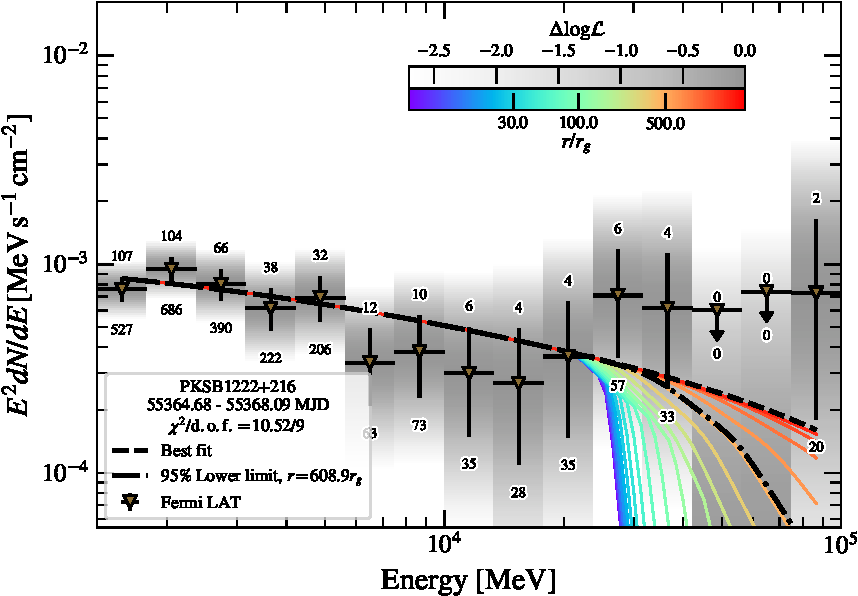
\includegraphics[width=0.32\linewidth]{figures/sed_PKSB1222+216_t001_LogParabola_3min_ring_emin1000.pdf} &
    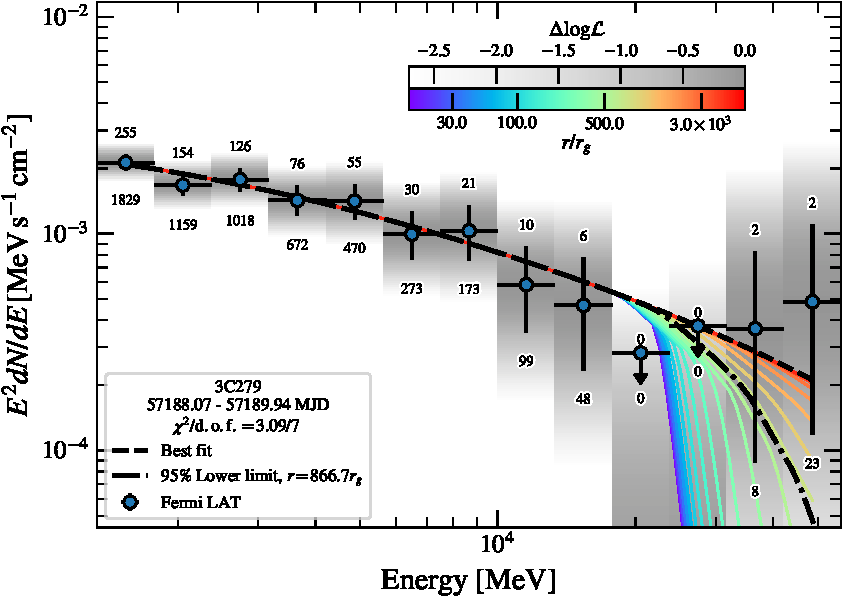
\includegraphics[width=0.32\linewidth]{figures/sed_3C279_t001_LogParabola_3min_ring_emin1000.pdf} & 
    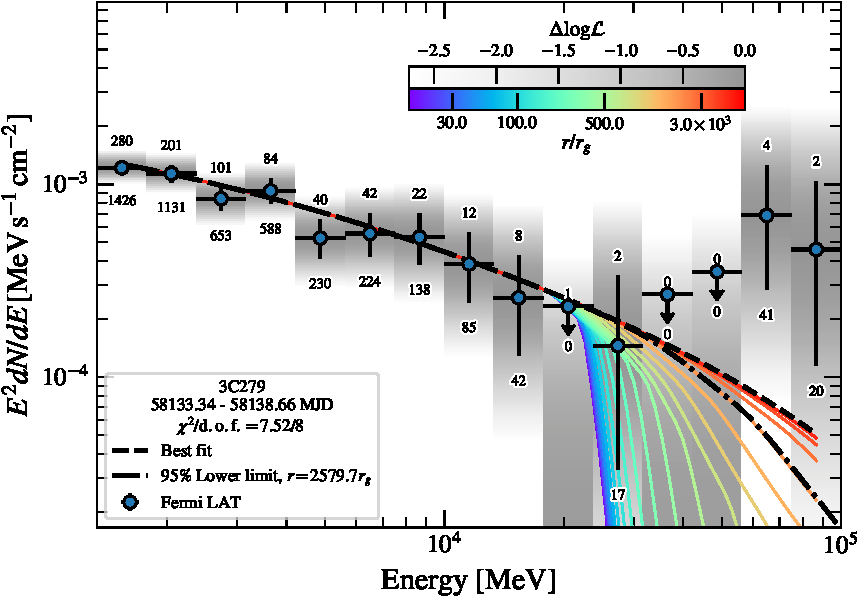
\includegraphics[width=0.32\linewidth]{figures/sed_3C279_t003_LogParabola_3min_ring_emin1000.pdf}\\
    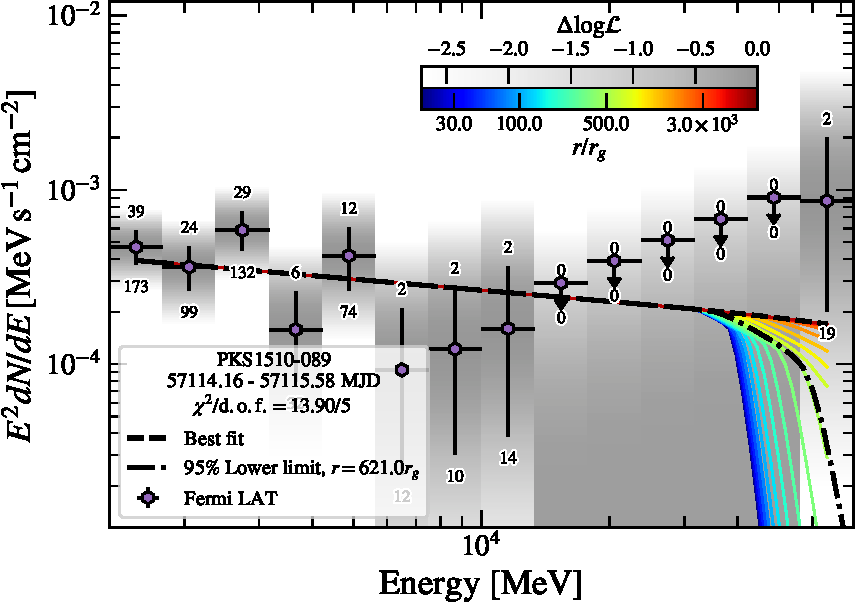
\includegraphics[width=0.32\linewidth]{figures/sed_PKS1510-089_t005_LogParabola_3min_ring_emin1000.pdf} &
    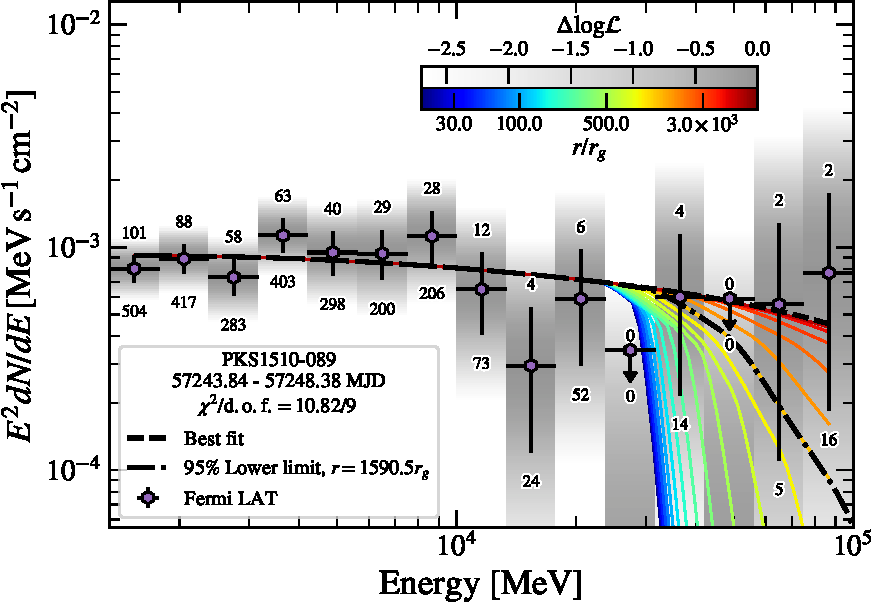
\includegraphics[width=0.32\linewidth]{figures/sed_PKS1510-089_t006_LogParabola_3min_ring_emin1000.pdf} & 
    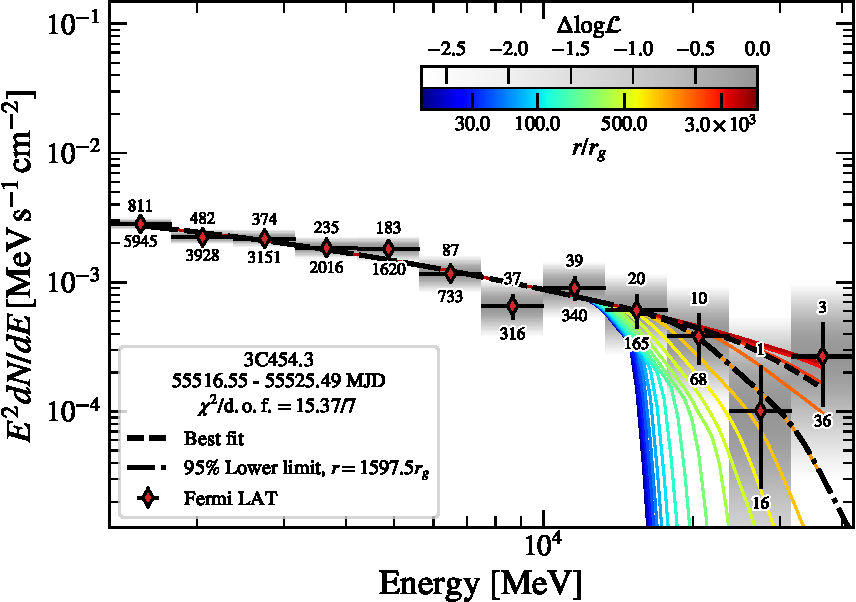
\includegraphics[width=0.32\linewidth]{figures/sed_3C454p3_t001_LogParabola_3min_ring_emin1000.pdf}\\
    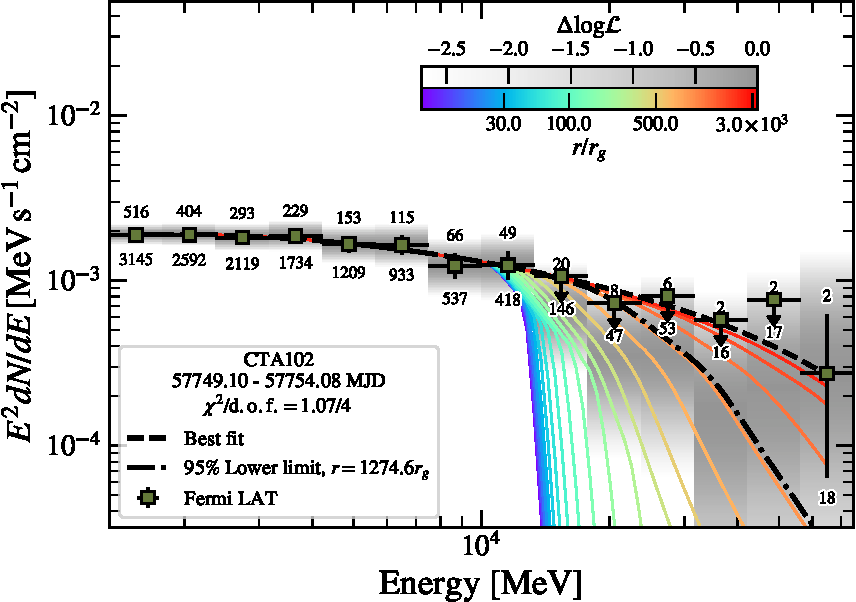
\includegraphics[width=0.32\linewidth]{figures/sed_CTA102_t002_LogParabola_3min_ring_emin1000.pdf} & 
    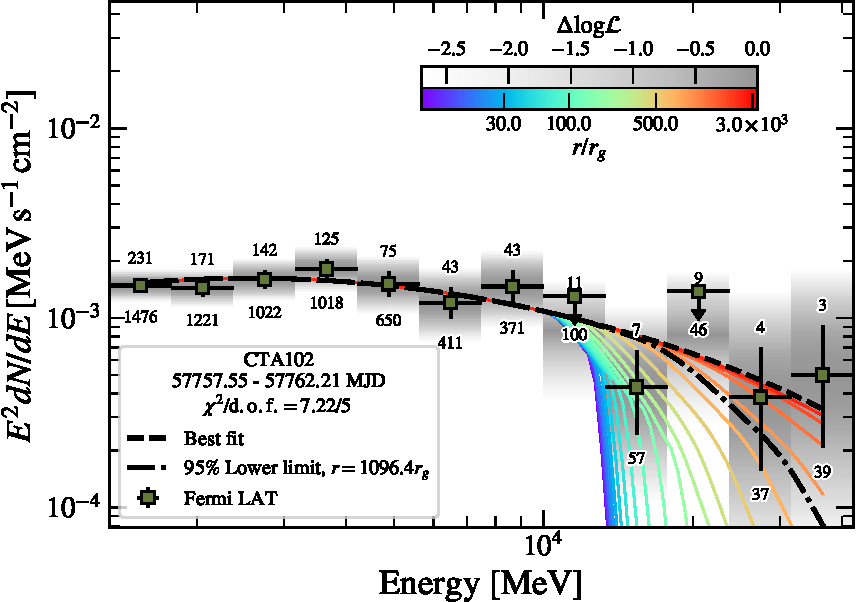
\includegraphics[width=0.32\linewidth]{figures/sed_CTA102_t003_LogParabola_3min_ring_emin1000.pdf} & 
    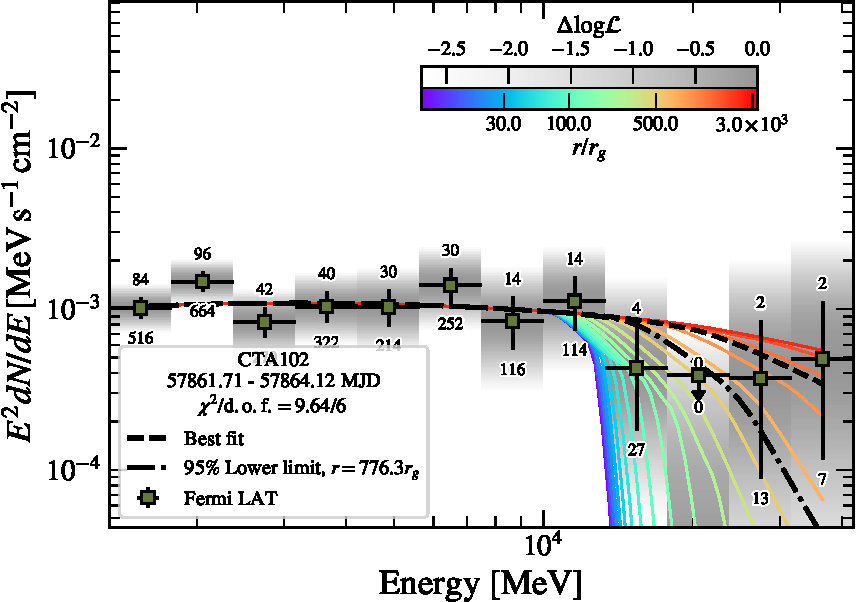
\includegraphics[width=0.32\linewidth]{figures/sed_CTA102_t004_LogParabola_3min_ring_emin1000.pdf}\\
    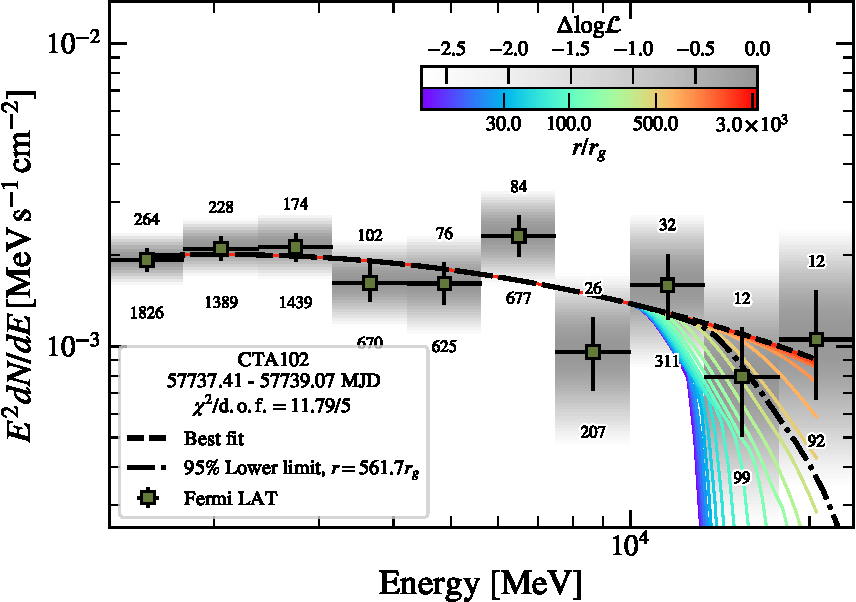
\includegraphics[width=0.32\linewidth]{figures/sed_CTA102_t001_LogParabola_3min_ring_emin1000.pdf}
    \end{tabular}

    \caption{Log-parabola fits above 1\,GeV to bright \gray flares detected at energies that correspond to a attenuation in the BLR of at least 20\,\% (for $r = 10^{-2}R_{\mathrm{Ly}\alpha}$). The attenuation due to the interactions with BLR photons (assuming the ring geometry) is shown as colored lines. The best fit (95\,\% lower limit on $r$) is shown as a black dashed (dash-dotted) line. 
    The fit uses the bin-by-bin likelihood curves shown as gray bands. The numbers below and above the flux points show the $\mathrm{TS}$ values  with which each bin is detected and the number of \Grays associated with the source at a probability $>85\,\%$, respectively.}
    \label{fig:seds}
\end{figure*}

For both tested BLR geometries, the best-fit value of $r$ is always close to or coincides with the maximum tested value, $r = 10R_{\mathrm{Ly}\alpha}$, and hence no significant absorption is found (dashed black lines in Figure~\ref{fig:seds}). Consequently,  we use \textsc{Minos} to derive the profile likelihood as a function of $r$ from which we determine the 95\,\% lower limit on $r$, $r_\mathrm{lim}$ (dash-dotted black lines). 
The limit values are reported for each flare in Figure~\ref{fig:blr_limits} and  summarized in Table~\ref{tab:blrabs} for the ring BLR geometry and log-parabola spectrum.
Assuming instead a power law with super-exponential cut-off yields consistent results. 
For the BLR shell geometry the lower limits are a factor of $\sim2$-$3$ higher because this geometry predicts stronger absorption~\citep{finke2016}. The ring geometry is therefore the conservative choice. 

As can be seen from Table~\ref{tab:blrabs} and Figure~\ref{fig:blr_limits} the limits are of the order of $r_\mathrm{lim}\sim10^{17}$cm which translates to a distance close to or even beyond the Ly$\alpha$ emitting ring and consequently the BLR itself. In terms of gravitational radii, the emission regions are located at distances of at least $\sim10^3r_g$. 
Table~\ref{tab:blrabs} also reports the energy of the highest energy photon (HEP) associated with the FSRQ with at least $99\,\%$ probability. For all but one source, this energy is larger than the energy where the optical depth due to absorption in the BLR exceeds $\tau_{\gamma\gamma}^\mathrm{BLR} > 1$ (assuming $r = r_\mathrm{lim}$).
Our limits generally agree with the results of \citet{2018MNRAS.477.4749C}, who could limit the maximum value of $\tau_{\gamma\gamma}^\mathrm{BLR}$ to be around $\sim 1$ for 3C454.3 and PKSB1222+216 and $\sim 0.2$ for CTA102. 

The limits sensitively depend on the detection of the source at energies as high as possible. To ensure that the detections are not spuriuos, we also report the detection significance and the number of detected \Grays (associated with the source with a probability $>85\,\%$) for each energy bin below and above the flux points in Figure~\ref{fig:seds}, respectively. The highest energy bins only contain a handful of source photons (1-4), which underlines the necessity to use the full Poisson likelihood information. 
Nevertheless, the source detections in these energy bins correspond to significances $\sim \sqrt{\mathrm{TS}}$ $\gtrsim 4\,\sigma$.
The reason is that in the considered energy interval and short time spans (cf. Table~\ref{tab:blrabs}) the number of expected background events is small. 

\begin{figure}
    \centering
    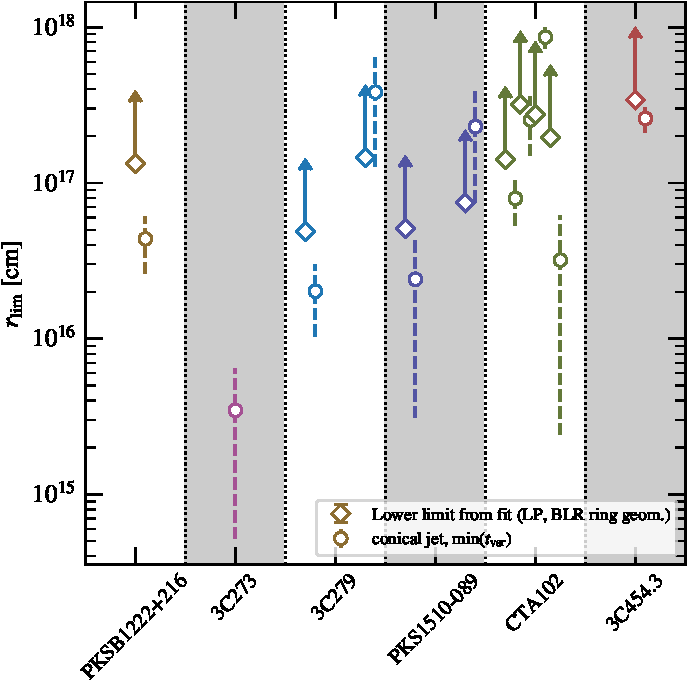
\includegraphics[width = .9\linewidth]{figures/limits.pdf}
    \caption{Lower limits on the distance $r$ of the \gray emitting region to the central black hole. Limits from fits to \gray spectra are shown as diamonds, values derived from variability considerations are shown as bullets. }
    \label{fig:blr_limits}
\end{figure}

\begin{deluxetable*}{ccccccc|ccc}
\tablewidth{0pt}
\tablecaption{ \label{tab:blrabs}Results from BLR absorption fits to \gray spectra.}
\tablehead{\colhead{$t_0$} & \colhead{$\Delta t$}  & \colhead{$r_\mathrm{lim}$} & 
\colhead{$r_\mathrm{lim}$} & \colhead{$r_\mathrm{lim}$} &  \colhead{$E_\mathrm{HEP}$}  & \colhead{$E_{\tau_{\gamma\gamma} = 1}$} & \colhead{$t_\mathrm{cool,~BLR}$}  &
\colhead{$t_\mathrm{cool,~dt}$}  & \colhead{$\tau_\mathrm{decay}$}\\
{} [MJD] & [days] & $[10^{17}\mathrm{cm}]$ & $[R_{\mathrm{Ly}\alpha}]$ & $[r_g]$ & [GeV] & [GeV] &  [mins] & [hours] & [hours]
}
\startdata
\hline
\multicolumn{10}{c}{PKSB1222+216}\\
\hline
55364.68 & 3.42 & 1.33 & 1.40 & 609 & 75.39 & 69.69 & 8.2 & 26.8 & $47.4\pm8.3$\\
\hline
\multicolumn{10}{c}{3C279}\\
\hline
57188.07 & 1.87 & 0.49 & 0.64 & 867 & 56.03 & 42.91 &  2.7 & 19.0 & $0.5\pm0.9$\\
58133.34 & 5.32 & 1.45 & 1.91 & 2580 & 92.56 & 107.91& 9.0 & 19.0 & $8.2\pm6.3$\\
\hline
\multicolumn{10}{c}{PKS1510-089}\\
\hline
57114.16 & 1.42 & 0.51 & 0.66 & 1088 & 66.54 & 54.99 & 0.6 & 4.5 & $0.4\pm0.3$\\
57243.84 & 4.53 & 0.74 & 0.97 & 1591 & 75.93 & 65.39 & 0.8 & 4.5 & $44.4\pm9.4$\\
\hline
\multicolumn{10}{c}{CTA102}\\
\hline
57737.41 & 1.67 & 1.41 & 0.86 & 562 & 36.25 & 21.23 & 1.0 & 6.4 & $0.3\pm0.5$\\
57749.10 & 4.99 & 3.20 & 1.95 & 1275 & 73.80 & 37.94& 2.8 & 6.4 & $8.7\pm1.2$ \\
57757.55 & 4.66 & 2.76 & 1.67 & 1096 & 39.19 & 32.38& 2.2 & 6.4 & $24.6\pm2.3$ \\
57861.71 & 2.42 & 1.95 & 1.18 & 776 & 34.73 & 24.94& 1.4 & 6.4 & $1.2\pm0.7$ \\
\hline
\multicolumn{10}{c}{3C454.3}\\
\hline
55516.55 & 8.93 & 3.19 & 1.36 & 1598 & 41.19 & 28.73& 4.2 & 16.8 & $2.6\pm1.0$ \\
\enddata
{
\tablecomments{Highest energy photons are given for source probabilities $> 0.99$. The decay times are given for the flare component with highest peak flux as determined in the fit to the orbital light curves in Section~\ref{sec:results-local}.
For the cooling times, an observed \gray energy of $10^{8.5}\,\mathrm{eV} \approx 316\,$MeV is assumed. }
}
\end{deluxetable*}

We also compare the limits from fits to \gray spectra to considerations from variability arguments in Figure~\ref{fig:blr_limits}.
If the emission region $R'_\mathrm{blob}$ (the prime denotes the co-moving frame) is causally connected during the flare, the shortest variability time $t_\mathrm{var}$ sets a lower limit on its size \citep[e.g.,][]{2008MNRAS.384L..19B}:
\begin{equation}
    R'_\mathrm{blob} \leqslant \frac{ct_\mathrm{var}\delta_\mathrm{D}}{1+z},
    \label{eq:rblob}
\end{equation}
where $\delta_\mathrm{D} = \Gamma^{-1}_\mathrm{L}(1 + \beta\cos\theta_\mathrm{obs})^{-1}$ is the Doppler boost factor with the bulk Lorentz factor of the flow, $\Gamma_\mathrm{L}$, $\beta = \sqrt{1 - \Gamma_\mathrm{L}^{-2}}$ the associated velocity, and $\theta_\mathrm{obs} $ is the angle between the line of sight and the jet axis.
Under the assumption of a conical jet with opening angle $\theta_\mathrm{j} \sim \Gamma^{-1}_\mathrm{L}$, we obtain an upper limit on the distance to the black hole, $r \sim R'_\mathrm{blob}\Gamma_\mathrm{L} \equiv r_\mathrm{j}$.
The values are plotted in Figure~\ref{fig:blr_limits} for the minimum of the rise and decay times of the brightest flares found in Figure~\ref{fig:gti}.
The average values for $\delta_\mathrm{D}$ and $\Gamma_\mathrm{L}$ obtained from Very Long Baseline Array monitoring observations are used \citep[see also Table~\ref{tab:src-select}]{2017ApJ...846...98J}  and the total  uncertainty is obtained by summing the uncertainties on $\delta_\mathrm{D}$, $\Gamma_\mathrm{L}$, and the fit uncertainty of $t_\mathrm{var}$ in quadrature.
In general, we find that $r_\mathrm{lim} \gtrsim r_\mathrm{j}$ indicating that the emission regions are at larger distances to the black hole than predicted from the conical jet scenario.  

In our BLR model, we use a simplified BLR geometry and do not include the hydrogen or HeII recombination continua or emission lines of the HeII Ly series~\citep[as done in, e.g.,][]{2010ApJ...717L.118P,2014ApJ...794....8S}. 
Comparing the optical depths of our model to results of the sophisticated modeling of~\citet[see in particular their Figure~11]{2017MNRAS.464..152A}, who describe the BLR as a collection of ionized gas clouds irradiated by the accretion disk, we find that our values of $\tau_{\gamma\gamma}^\mathrm{BLR}$ reach unity at energies a factor of $\sim1.5$ higher, but around 100\,GeV the optical depth in the two models is similar. 
Also, the BLR model of \citet{finke2016} re-produces the trend observed in the sophisticated model that the absorption sets in at higher energies and is overall weaker for larger values of $r$. 
As we do not observe significant cut-offs in the spectra, we therefore conclude that the ring geometry adopted here provides a conservative limit on $r$. 

Furthermore, evidence exists that the the luminosity of BLR emission lines is variable in 3C454.3, PKS1510-089, and PKSB1222+216~\citep{2013ApJ...763L..36L,2015ApJ...804....7I} and correlates with the \gray emission~\citep{2013ApJ...763L..36L,2015IAUS..313...43L}, which could indicate that \Grays are produced through inverse Compton scattering with BLR photons (see also Section~\ref{sec:tcool}).  
Additionally, \citet{2013ApJ...763L..36L} find that the BLR brightening coincides with the passage of a superluminal jet component through the radio core, which could indicate that BLR clouds are located at larger distances, $\gtrsim 1\,$pc, then assumed here.
A brighter BLR emission during \gray flares and BLR material located at larger distances would mean stronger \gray attenuation, which would shift our limits to even larger distances. 

\subsubsection{Jet-shielding by a plasma sheath}
\label{sec:plasma-sheath}

In view of the severity of these constraints, it is worth considering radical alternatives to the standard model of FSRQ \gray emission. The first possibility is that the inner jet is actually shielded from external soft photons. One way in which this can happen is if the broad line-emitting clouds derive from the accretion disk and are propelled to radii $\sim0.1-1\,{\rm pc}$ by the centrifugal action of magnetic field lines attached to the accretion disk \citep{emmering:1992mac,1994ApJ...434..446K,bottorf:1997dyn}. The magnetic field channels the cool gas along outward trajectories with speeds $\sim0.03c$ including some rotation.  Individual gas clouds can be confined transversely by magnetic pressure but will cool as they expand. 

Generic BLR models have filling factors $\sim10^{-5}-10^{-4}$ and covering factors $\sim0.1$. Now, suppose that some of these clouds derive from the inner disk and are attached to the toroidal field lines that are thought to collimate the jet. They will be illuminated from the outside and their thermal state will be a balance between photoionization heating and expansion and radiative loss. In order for a \gray of energy $E_\gamma$ to escape from the inner jet we must have efficient shielding out to the $\gamma$-sphere  \citep{1995ApJ...441...79B} defined by the unshielded photons. If this outflow can remain cool enough, a column density $\Sigma\gtrsim\Sigma_{\rm shield}\sim5\times10^{-3}E_{X\,\rm keV}^{2.5}\,{\rm g\,cm}^{-2}$, for $0.014\lesssim E_{X\,\rm keV}\lesssim10$ suffices to shield the jet from photons of energy $E_{X\,\rm keV}$. It is unlikely that this sheath can be neutral enough to shield the UV down to the Lyman continuum close to the hole. Prominent line photons, notably Ly$\alpha$, should also be shielded. We can express $\Sigma_{\rm shield}$ in terms of $E_\gamma$ at threshold for pair production, $\Sigma_{\rm shield}\sim2\times10^{-4}E_{\gamma\,\rm GeV}^{-2.5}\,{\rm g\,cm}^{-2}$ for $0.03\lesssim E_{\gamma\,{\rm GeV}}\lesssim20$ and for sufficiently large jet radius. 

Next, suppose that the cylindrical radius of the sheath at the $\gamma$-sphere is $10^{15}s_{\gamma{\rm sphere}\,15}\,{\rm cm}$, (typically $\sim0.1$ of the jet radius). The discharge associated with the shielding gas is then $\dot M_{\rm sheath}\sim10^{-5}s_{\gamma{\rm sphere}\,15}E_{\gamma\,\rm GeV}^{-2.5}\,{\rm M}_\odot\,{\rm yr}^{-1}$, which is quite modest for the energies of interest. An observer situated on the jet axis should be able to observe $\gamma$-rays from very close to the black hole, at radii much smaller than that of the $\gamma$-sphere, where their observed variability timescales can be as short as minutes after correcting for relativistic time travel effects. Of course, there may be some opacity due to synchrotron photons emitted at smaller jet radii and beamed along the jet but, again this need not be severe. Note that photons with energy below the Lyman continuum, including optical and infrared photons, should permeate the jet at all radii and so this model implies that there should not be rapid \gray variability with $E_{\gamma}\gtrsim30/(1+z)\,{\rm GeV}$ from FSRQ. The rapid variability seen  at TeV energy in some BLL arises because these sources like a strong UVX continuum and the hole masses are smaller.

\subsection{Considerations from radiative cooling}
\label{sec:tcool}
\subsubsection{Broad emission line radiation}
With the limits on $r$ it is possible to derive constraints on the energy density of external photon fields in the co-moving frame, which could be responsible for the \gray emission due to inverse-Compton (IC) scattering with relativistic electrons in the emission region. 
Because the cooling time depends on the energy density and in turn on $r$, a comparison between the predicted IC cooling times with the observed decay times can provide further information on where the \Grays are emitted.
We first focus on the BLR photon field but the discussion also applies for IC scattering with photons of the dust torus, which we will discuss at the end of this section.

In the galaxy frame, the energy density of the BLR in the ring geometry is approximately given by Eq.~\ref{eq:u-blr}, and hence the photon number density is $n_\mathrm{BLR} \approx u_\mathrm{BLR} / \epsilon_{\mathrm{Ly}\alpha}\sim10^{9}\,\mathrm{cm}^{-3}$.
Assuming that the BLR photon field is isotropic and in the limit $\Gamma_\mathrm{L} \gg 1$, the energy density in the co-moving frame becomes:
$u'_\mathrm{BLR} = (4/3)\Gamma_\mathrm{L}^2 u_\mathrm{BLR}$~\citep{1994ApJS...90..945D,2002ApJ...575..667D}.
We calculate the energy loss of the electrons, $\dot{\gamma}_\mathrm{BLR}'$, due to IC scattering in the co-moving frame numerically, in order to incorporate Klein-Nishina   effects following \citet{1970RvMP...42..237B}.
The observed cooling time is then given by
\begin{equation}
    t_\mathrm{cool,BLR} = \frac{1 + z}{\delta_\mathrm{D}} \frac{\gamma'}{\dot{\gamma}'_\mathrm{BLR}}.
    \label{eq:tcool}
\end{equation}
In the Thomson regime, this becomes
\begin{equation}
    t_\mathrm{cool,BLR} = \frac{1+z}{\delta_\mathrm{D}}\frac{3m_ec^2}{4c\sigma_\mathrm{T}u_\mathrm{BLR}'\gamma_\mathrm{BLR}'},
    \label{eq:tcool-thomson}
\end{equation}
where $m_e$ is the electron mass and $\sigma_\mathrm{T}$ the Thomson cross section. 
In what follows, we approximate the electron Lorentz factor with~\citep[e.g.,][]{2009herb.book.....D,finke2016}
\begin{equation}
    \gamma'_\mathrm{BLR} = \frac{1}{ \delta_\mathrm{D}}\sqrt{\frac{E_\mathrm{obs,BLR}(1+z)}{2\epsilon_{\mathrm{Ly}\alpha}}},
    \label{eq:gammaprime}
\end{equation}
where $E_\mathrm{obs,BLR}$ is the observed \gray energy of IC scattered BLR photons. 
From Eqs.~\ref{eq:u-blr}, \ref{eq:tcool-thomson}, and \ref{eq:gammaprime} it becomes clear that the cooling time scales as $t_\mathrm{cool, BLR}\propto r^2 \Gamma^{-2}$, i.e., the cooling becomes less efficient for large distances. 
Furthermore, if the \gray emission is produced very far away from the BLR, the external photons will appear as a point source illuminating the emission region from behind, so that $u'_\mathrm{BLR} = (1/4)\Gamma^{-2} u_\mathrm{BLR}$,~\citep{1994ApJS...90..945D} leading to an additional decrease of the cooling time. 
The BLR cooling time for one flare of CTA102 is shown for $r=r_\mathrm{lim}$ and $r = 1\,$pc as a function of $\gamma'$ and $E_\mathrm{obs,BLR}$ in Figure~\ref{fig:tcool}  (black solid and dash-dotted lines, respectively), assuming again the average values for $\delta_\mathrm{D}\sim31$ and $\Gamma_\mathrm{L}\sim22$. 
Klein-Nishina effects become important for $\gamma'_\mathrm{BLR} \gtrsim 2\times10^3$ or $E_\mathrm{obs,BLR}\gtrsim1\,$GeV and a clear departure from the Thomson regime in which 
$t_\mathrm{cool}\propto(\gamma_\mathrm{BLR}')^{-1/2}$ (dashed and dotted black lines) becomes visible.
The decay times derived from the fit of the two bright flares of CTA102 around MJD 57738 are shown is dark green squares (see the first solid horizontal line in the panel in the 4th row and 2nd column in Figure~\ref{fig:gti}), where one decay time is shown as an upper limit due to its large uncertainty. 
If the decay is indeed caused by IC scattering with BLR photons, a distance of $r\sim1\,$pc is still compatible with the observed decay times. 
Similar conclusions can be drawn for the other sources. 
We provide the cooling times at 300\,MeV and the shortest decay times in Table~\ref{tab:blrabs}.

Figure~\ref{fig:tcool} also shows the variability time $t_\mathrm{var}$ derived for the sub-orbital period in Section~\ref{sec:sub-gti}, which is, however, in the rising part of the flare (cf. Figure~\ref{fig:lc_minutes}). If equally short decay times were observed, this would suggest a distance $r \sim r_\mathrm{lim}$. 

\begin{figure}
    \centering
    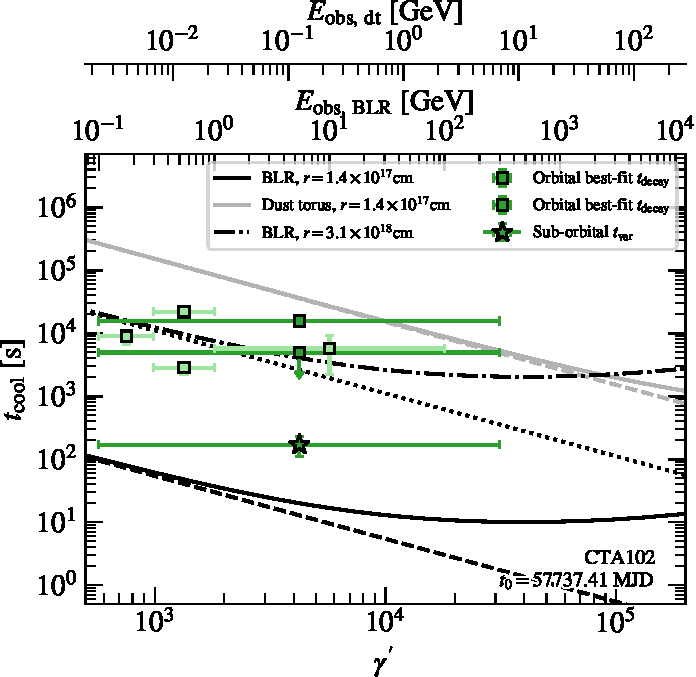
\includegraphics[width = .9\linewidth]{figures/tcool_CTA102_t001_LogParabola_ring.pdf}
    \caption{Cooling times for IC scattering with BLR photons and photons from the dust torus for one flaring episode of CTA102. Also shown are observed decay times for the full energy range, energy dependent light curves, and sub-orbital light curves.
    Note that the observed decay times are plotted with respect to IC scattering with BLR photons. For scattering with photons from the dust torus, the points need to be shifted to higher values of $\gamma'$ to match $E_\mathrm{obs,dt}$ (see second $x$-axis on the top of the figure).}
    \label{fig:tcool}
\end{figure}

  
As noted by \citet{2012ApJ...758L..15D}, the energy dependence of the cooling times could  further reveal the dominant photon field responsible for IC scattering: while Klein-Nishina effects become important already at 1\,GeV for scattering with BLR photons, the Thomson regime should be valid to higher energies for IC scattering with photons of the dusty torus (dt). 
Following again~\citet{finke2016}, we assume that the torus also has a ring geometry and emits monochromatic photons with energy $\epsilon_\mathrm{dt} = 2.7 k_B T_\mathrm{dt}$ with $k_B$ the Boltzmann constant and $T_\mathrm{dt} = 1000\,$K. 
The sublimation radius of the dust torus, $R_\mathrm{dt} = 3.5\times10^{18}\,\mathrm{cm}(L_\mathrm{disk}/10^{45}\,\mathrm{erg}\,\mathrm{s}^{-1})^{1/2}(T_\mathrm{dt}/10^3\,\mathrm{K})^{-2.6}$ is used as the ring radius. 
Making the appropriate substitutions in Eqs.~\ref{eq:u-blr}, \ref{eq:tcool}-\ref{eq:gammaprime}, we plot the cooling time $t_\mathrm{cool,dt}$ for $r = r_\mathrm{lim}$ as a grey line in Figure~\ref{fig:tcool} (note the additional $x$-axis since $E_\mathrm{obs, BLR} \neq E_\mathrm{obs,dt}$). 
Indeed, Klein-Nishina effects only become relevant at $E_\mathrm{obs,dt} \gtrsim 10^2\,$GeV or $\gamma' \gtrsim 10^5$. The cooling times at $E_\mathrm{obs,dt} = 316\,$MeV are also provided in Table~\ref{tab:blrabs}.

To further investigate the energy dependence of the decay times, we split the energy range of our analysis into three energy bins, 
 from 100\,MeV-300\,MeV, 300\,MeV-1\,GeV, and 1\,GeV-100\,GeV and recompute the orbital light curves.
The energy bins are chosen as a compromise between number of bins and sufficient photon statistics in each bin. 
The light curves for which at least 2 BBs are identified in each energy bin are shown in Figure~\ref{fig:lcebins}.
We repeat the fits of the exponential profiles to the energy dependent light curves but allow only one flare profile per HOP group. 
The resulting decay times are also plotted in Figure~\ref{fig:tcool} (light green squares). Only for the 300\,MeV-1\,GeV energy bin the double peak of the flare is resolved and in general the fit qualities are rather poor with $\chi^2$ per degree of freedom between 1.67 and 2.26.
The steep $\chi^2$ curves also explain the rather small error bars on $\tau_\mathrm{decay}$. 
From the fit values we cannot draw a conclusion whether the decay times evolve with $(E_\mathrm{obs})^{-1/2}$ as expected in the Thomson regime.
Due to the lack of high photon statistics at energies beyond 10\,GeV where the differences in cooling times between the dust torus and BLR become more pronounced, we are not able to use the method suggested by \citet{2012ApJ...758L..15D} to determine the photon field dominating the IC scattering. 
This conclusion also holds for the other sources. 

\begin{figure*}
    \centering
    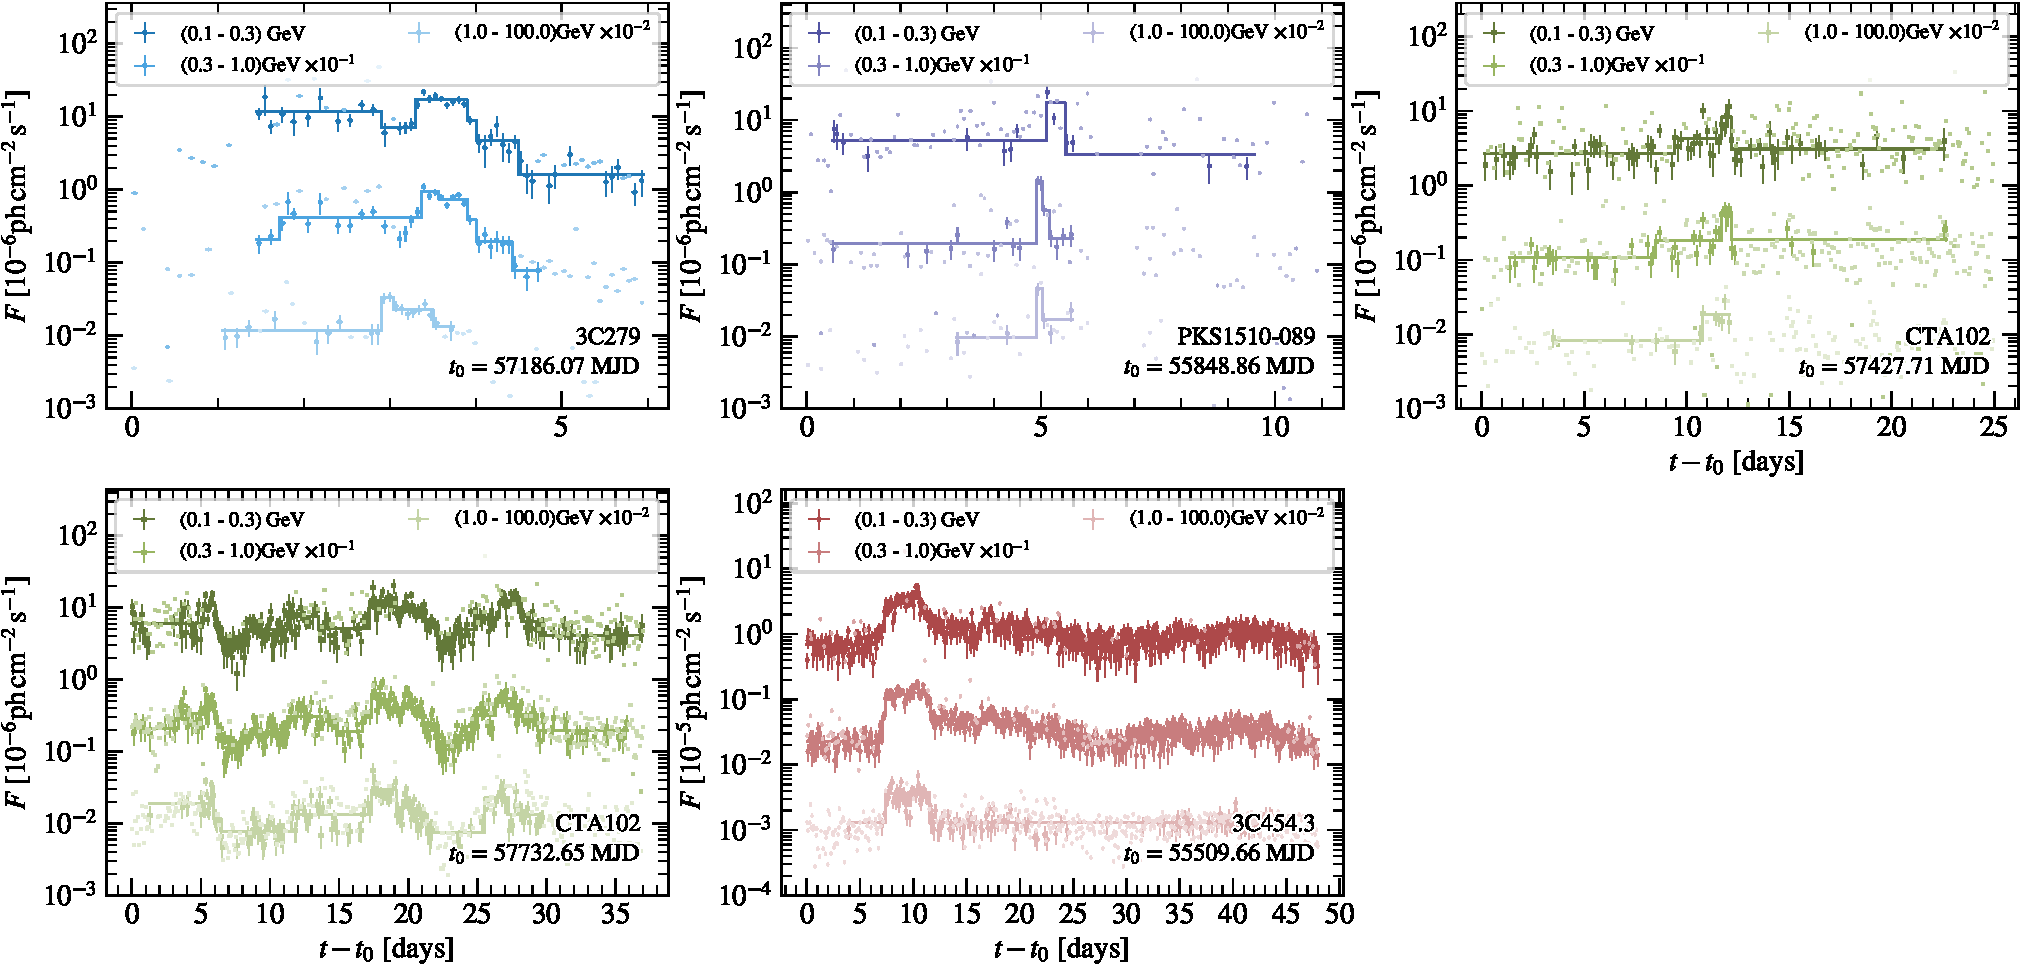
\includegraphics[width = .9 \linewidth]{figures/lc_ebins_ts9.pdf}
    \caption{\fermiLAT orbital light curves for three energy bins. The same time binning as in Figure~\ref{fig:gti} is used. The thick colored lines indicate the BB representation. Only light curves are shown for which at least two BBs are identified for each energy bin. The fluxes of the light curves of the energy bins 0.3-1\,GeV and 1-100\,GeV are shifted by $10^{-1}$ and $10^{-2}$, respectively, for better visibility. }
    \label{fig:lcebins}
\end{figure*}

Interestingly, the BBs for the energy dependent light curves of the flares of 3C279, PKS1510-089, and the last flare of CTA102 seem to show time lags between the energy bands, with the high-energy emission leading the low-energy \Grays.
For the 3C279 flare around MJD 57188, \citet{2015ApJ...808L..48P} could not find any time lags between the energy bins 0.1-1\,GeV and above 1\,GeV using the $Z$-transformed discrete correlation function \citep[DCF;][]{1997ASSL..218..163A,2013arXiv1302.1508A}.
Using the same methodology, we show the DCFs for our energy dependent light curves with at least 2 BBs per energy bin in Figure~\ref{fig:zdcf}.
We mark the time lags $\tau$ with horizontal lines at the maximum DCF values if $\mathrm{max}(\mathrm{DCF}) > 2 \sqrt{\mathrm{Var}(\mathrm{DCF})}$.
In contrast to \citet{2015ApJ...808L..48P}, we find evidence that the emission above 1\,GeV leads the emission at lower energies with $\sim 0.1$ days. 
However, from the fits to the light curves, the decay time at higher energies is actually longer ($0.45\pm0.16$ days above 1\,GeV versus $0.22 \pm 0.03$ between 0.1 and 0.3\,GeV). 
Therefore, the lag might not be associated with cooling but rather with a changing particle injection. 
From the spectral variation (Figure~\ref{fig:specvar}) it seems that the time bin before the peak of the flare has a harder spectrum, however, the uncertainties are too large to draw firm conclusions.
For the CTA102 flare around MJD 57758 we also find that the high energy emission is leading, whereas for the flare at MJD 57749 the picture is reversed. 
For 3C454.3 the DCF also indicates that the low-energy emission is leading the high-energy emission, again suggesting that these lags are connected to the injection of particles rather than radiative cooling.

\subsubsection{Synchrotron \Grays}
\label{sec:gammasync}

A second alternative to the standard model is that the \gray emission mechanism is electron synchrotron radiation \citep{TheFermi-LAT:2016dss}, not inverse Compton scattering as usually supposed \citep[e.g.,][]{Madejski:2016oqg}.
Electron synchrotron radiation is mostly dismissed because there is a $\sim70\,{\rm MeV}$ radiation reaction limit on the \gray energy in the comoving frame \citep[e.g.,][]{1975ctf..book.....L,blandford:2017mag}. However, if there is sufficient plasma entrainment beyond the outer light cylinder of the black hole magnetosphere, the dominant, positively-charged particles in the jet will be protons even after allowing for some additional pair production. Large, electric field components, along the magnetic field, may be created through a dynamical untangling of large magnetic flux ropes at relativistic speed --- magnetoluminescence --- and, when combined with charge starvation, can lead to a conversion of electromagnetic energy to relativistic particles and \Grays at relativistic speed across much larger volumes than can be processed by magnetic reconnection. 

Under these circumstances, half of the electromagnetic energy that is dissipated should go into the protons, which can be accelerated to much higher energy than the electrons. For an electromagnetic jet of power $L_{\rm jet}=10^{45}L_{\rm jet\,45}\,{\rm erg\,s}^{-1}$ bulk Lorentz factor $\Gamma_{\rm L}=10\Gamma_{\rm L1}$ and width $s=10^{15}s_{15}\,{\rm cm}\sim r/\Gamma_{\rm L}$, the comoving magnetic field strength is $B'\sim30L_{\rm jet\,45}^{1/2}s_{15}^{-1}\Gamma_{\rm L1}^{-1}\,{\rm G}$, the comoving accelerating electric field strength could be as large as $E'_{\rm max}\sim1L_{\rm jet\,45}^{1/2}s_{15}^{-1}\Gamma_{\rm L1}^{-1}\,{\rm MV\,m}^{-1}$ and the total potential difference across the jet could be as large as $V_{\rm max}\sim100\,L_{\rm jet\,45}^{1/2}\,{\rm EV}$. 

Proton acceleration is likely to be limited by the Bethe-Heitler process where a photon of energy $E''_\gamma>1\,{\rm MeV}$ in the proton rest frame creates an electron-positron pair with a cross section that rises slowly from $\sigma_{\rm BH}\sim1\,{\rm mb}$ at $E_\gamma''\sim5\,{\rm MeV}$ to $\sim 10\,{\rm mb}$ at $E_\gamma''\sim1\,{\rm GeV}$ \citep[e.g.,][]{2009herb.book.....D}. Pions will be created at higher energy when $E''_{\gamma}\gtrsim150\,{\rm MeV}$ and could be responsible for VHE neutrino emission but need not concern us here. 

If we focus on the $\sim3\,{\rm min}$ flare in 3C279 with %$r_g\sim1.5\times10^{14}\,{\rm cm}$, 
$r_g\sim5.6\times10^{13}\,{\rm cm}$, 
$L_{\rm jet\,45}\sim1$, and assume that $\Gamma_{\rm L}\sim10$, then the constraint of Equation~\ref{eq:rblob} suggests that the size of the emitting region associated with the flare is $R'_{\rm blob}\sim10^{14}\,{\rm cm}$. There is a second constraint in that the electromagnetic energy contained within the blob should be large enough to account for the amplitude of the flare. This suggests that $r\sim10^{16}\,{\rm cm}$, $s_{15}\sim1$ and a fraction $\sim0.01$ of the jet area is involved with this flare. 

Next, suppose that the inner jet is effectively shielded blueward of the Lyman continuum, and so the highest energy external photons in the jet originating from the accretion disk, with energy $E_{\rm UV}\sim10\,{\rm eV}$, will have a number density $n_{\rm UV}\sim10^{12}\,{\rm cm}^{-3}$ (assuming a distance where the photon density is the logarithmic mean between $10^9\,\mathrm{cm}^{-3}$ at $R_\mathrm{Ly\alpha}$ and the photon density of a black body with $T = 3\times10^4\,$K which gives $n\sim10^{15}\,\mathrm{cm}^{-3}$) and energy density $\sim10\,{\rm erg\,cm}^{-3}$, roughly a tenth the magnetic energy density. These photons will have energies $E_\gamma''\sim\Gamma_{\rm L}\gamma_p'E_{\rm UV}\sim100\,{\rm MeV}$, where $\gamma_p'\sim10^6$ is the proton Lorentz factor, in the comoving frame. Pairs will then be created at a rate $R'\sim\Gamma_{\rm L}n_{UV}\sigma_{\rm BH}\sim10^{-11}\,{\rm m}^{-1}$ in the comoving frame and the associated pairs will have energies $E_e'\sim \gamma_P'E_\gamma''\sim100\,{\rm TeV}$. The proton energy loss rate rate in the comoving frame is then $E_e'R'\sim1\,{\rm keV}\,{\rm m}^{-1}\propto\Gamma_L^2\gamma_P'^2$. The electric field needed to balance this loss is only $\sim10^{-3}$ of $E_{\rm max}'$. The proton acceleration/radiation lengths are then $\sim10^{14}\,{\rm cm}\sim R_{\rm blob}'$ and the protons can be maintained at $\sim\,{\rm PeV}$ energies for the duration of the flare.

The pairs will rapidly cool by synchrotron emission (inverse Compton scattering is strongly Klein-Nishina suppressed), radiating \Grays with comoving energy $\sim (E_e'/m_ec^2)^2 B' \sim 1\,{\rm GeV}$ and AGN frame energies boosted by a factor $\sim\Gamma_{\rm L}$ to energies $E_\gamma\lesssim10\,{\rm GeV}$. These \Grays are just below the threshold energy for pair production ($E_\gamma\sim25\,{\rm GeV}$) and should be visible when the line of sight is fully contained by the absorbing sheath. \Grays emitted below the jet $\gamma$-sphere will create more pairs which will emit lower energy \gray photons which should escape unimpeded. The overall process is electromagnetic and should be very efficient, unlike with photo-pion production where there will be neutrino and neutron losses. 

Electrons will also be directly and rapidly accelerated by the electric field to energies $\sim300\,{\rm GeV}$ until they are limited through radiating synchrotron \Grays of energy $\sim0.5\,{\rm MeV}$ in the AGN reference frame. These should escape unimpeded, with comparable power to the GeV \Grays and could be detectable. (Inverse Compton scattering is also Klein Nishina-suppressed but could significant.) In order to dissipate the energy at relativistic speed, the current density must be $\sim3\,\mu{\rm A\,m}^{-2}$ and the associated proton pressure would have to be $\sim100\,{\rm dyne\,cm}^{-2}$, comparable with the magnetic pressure at the height of the flare.

The  case of 3C279 is extreme and may require specialized, not generic, conditions including especially the necessary efficacy of the shielding at photon energies above the Lyman continuum. However, even in this case, it seems that the surprisingly rapid variation observed can be explained making simple, though not mandatory, assumptions. Modeling the larger sample of variable FSRQ described here introduces many more possibilities. In particular, the presumption that the emission originates in a single ``zone'', while appropriate for an extreme flare is surely quite wrong when modeling a more slowly varying \gray spectrum. Most of the emission is likely to originate over a range of larger jet radii with lower radiation density. The details will be largely dictated by the interaction of the jet with the surrounding outflow and the dynamics of the jet electromagnetic field.

A fuller account of the processes involved will be presented elsewhere.

\begin{figure*}
    \centering
    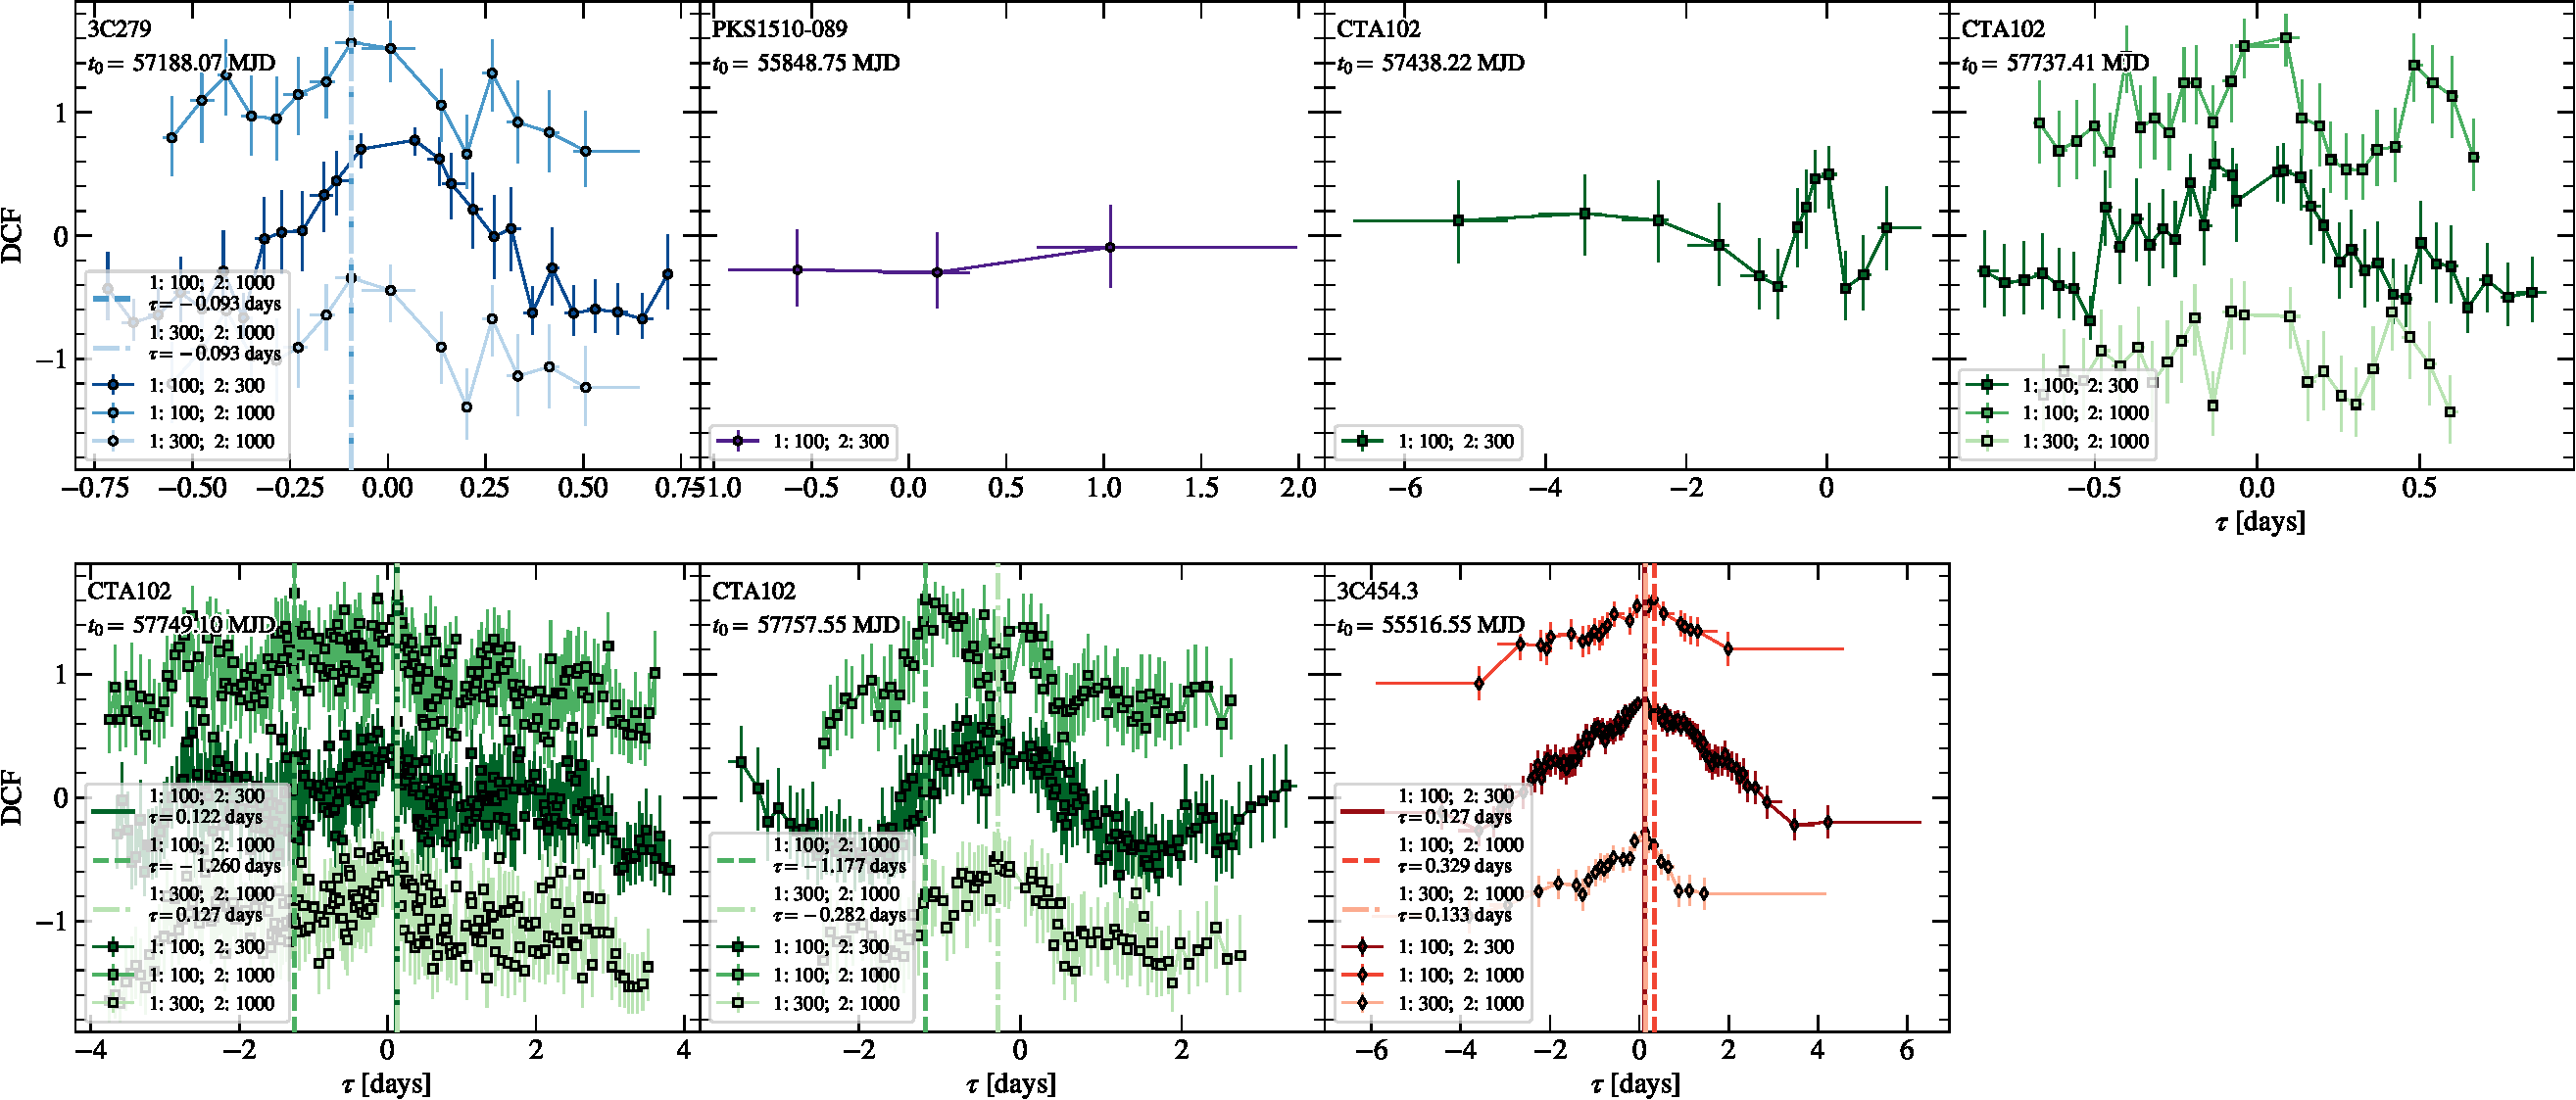
\includegraphics[width = .9 \linewidth]{figures/zdcf_ebins.pdf}
    \caption{Results for the DCF analysis for the light curves in Figure~\ref{fig:lcebins}. In order to detect time lags for single flares, the three flares of CTA102 starting at MJD 57733 are separated using the HOP groups. For time lags $\tau < 0$ the high-energy light curve leads the low-energy one. The DCFs between the energy bins (0.1-300\,MeV,1-100\,GeV) and (0.3-0.3\,GeV,1-100\,GeV) are shifted by $\pm 1$ for better visibility. 
    Horizontal lines mark the maximum of the DCFs if $\mathrm{max}(\mathrm{DCF}) > 2 \sqrt{\mathrm{Var}(\mathrm{DCF})}$.}
    \label{fig:zdcf}
\end{figure*}

\subsection{Results from radio-\gray correlation analysis}
\label{sec:gammaradio}

Cross-correlating \gray light curves with radio light curves provides an alternative method to locate the \gray emitting region~\citep[e.g.,][]{2014MNRAS.441.1899F}.
Under the assumption that the flares are produced in a common compact emission  region moving down the jet~\citep[e.g.,][]{2014MNRAS.445..428M},
the distance $d_{\gamma,r\nu}$ between the 
the \gray sphere, where the \gray opacity due to, e.g., absorption in the BLR, becomes less than unity~\citep{1995ApJ...441...79B}, and the 
radio core, where synchrotron-self-absorption becomes negligible~\citep[][]{1981ApJ...243..700K}, 
can be estimated from the time lag between the light curves, 
\begin{equation}
    d_{\gamma,r\nu} = \frac{\Gamma\delta_\mathrm{D}\beta c\tau_{\mathrm{peak},\gamma,r\nu}}{1 + z},
    \label{eq:dgamma-r}
\end{equation}
where $\tau_{\mathrm{peak},\gamma,r\nu}$ is the time lag corresponding to a peak in the cross-correlation function between the \gray light curve and radio light curve obtained at frequency $\nu$.
Under the assumption that the radio emission lags the \Grays, the distance of the \gray emission region to the central black hole is thus $d_\gamma = d_{\mathrm{core},r\nu} - d_{\gamma,r\nu}$, where $d_{\mathrm{core},r\nu}$ is the position of the radio core at frequency $\nu$.
The core position itself is frequency dependent~\citep[the core shift effect, see, e.g.,][]{1998A&A...330...79L},
\begin{equation}
    d_{\mathrm{core},r\nu} = \frac{\Omega_{r\nu}}{\nu^{1/k_r}\sin\theta_\mathrm{obs}},
     \label{eq:core-shift1}
\end{equation}
where $k_r$ depends on the electron energy spectrum and the magnetic field in the emitting region~\citep{1981ApJ...243..700K} and
\begin{equation}
    \Omega_{r\nu} = 4.85\times10^{-9} \frac{\Delta r_\mathrm{mas} d_\mathrm{L}}{1 + z}\frac{\nu^{1/k_r}\nu_0^{1/k_r}}{\nu_0^{1/k_r}-\nu^{1/k_r}},
    \label{eq:core-shift2}
\end{equation}
where $d_\mathrm{L}$ is the luminosity distance and $\Delta r_\mathrm{mas}$ is the offset between the radio cores in milliarcseconds at frequencies $\nu$ and $\nu_0$. 
The offest is related to the time lag between two radio light curves $\tau_{\mathrm{peak},r\nu,r\nu_0}$ through 
$\Delta r_\mathrm{mas} = \mu \tau_{\mathrm{peak},r\nu r\nu_0}$, where $\mu$ is the jet proper motion. 

The proper motion along with the core position at 15\,GHz have been determined from
MOJAVE blazar monitoring program along using very large baseline interferometry \citep[VLBI][]{2012A&A...545A.113P,2016AJ....152...12L}.
The following distances $d_\mathrm{core,~15GHz}$ were determined  under the assumption that $k_r = 1$: for PKSB1222+216 $d_\mathrm{core,~15GHz}= 23.41\,$pc; for 3C279 $d_\mathrm{core,~15GHz}<7.88$\,pc; for PKS1510-089 $d_\mathrm{core,~15GHz} = 17.71\,$pc; for 
CTA102 $d_\mathrm{core,~15GHz} =46.7\,$pc; and for 3C454.3 $d_\mathrm{core,~15GHz} = 20.36\,$pc.
Dedicated analyses have also been carried out and found for 3C454.3 $k_r = 0.6$-$0.8$ and $d_\mathrm{core,~15GHz} \sim 38\,$pc and, since $d_{\mathrm{core},r\nu}\propto\nu^{-1/k_r}$,  $d_\mathrm{core,~43GHz} \sim 9\,$pc~\citep{2014MNRAS.437.3396K}. 
For 3C273 \citet{2013ARep...57...34V} find $k_r = 1.4$ and $d_{\mathrm{core},r\nu} = 134\nu^{-1/1.4}$ using radio observations at frequencies between 4.8 and 362 GHz.
Lastly, \citet{2015A&A...576A..43F} conducted VLBA observations of CTA102 ranging from 5\,GHz to 86\,GHz and found $k_r = 1.0$ as a best-fit value and $d_{\mathrm{core,~86GHz}}\sim7\,$pc.
Provided that we can estimate $\tau_{\mathrm{peak,15GHz},r\nu}$, it is possible with the above results to estimate the core position at an arbitrary radio frequency using Eqs.~\ref{eq:core-shift1} and \ref{eq:core-shift2}.
In order to arrive at an estimate for $d_\gamma$ the only remaining task is to perform a cross correlation study between \gray and radio light curves.

We search for time lags between the \fermiLAT light curves and radio light curves obtained with the Owens Valley Radio Observatory (OVRO) at 15\,GHz, the Atacama Large submillimeter/millimeter Array (ALMA) between 84 and 116\,GHz (Band 3, 3.6\,mm-2.6\,mm), and the Submillimeter Array (SMA) at 230\,GHz (1.3\,mm). 
All of the studied FSRQs are included in an ongoing blazar monitoring program at OVRO~\citep{2011ApJS..194...29R} and SMA~\citep{2007ASPC..375..234G}, and also serve as calibrators for SMA and ALMA~\citep{2018MNRAS.478.1512B} at mm wavelengths.\footnote{Data from the observatories are available at \url{http://www.astro.caltech.edu/ovroblazars}, \url{https://almascience.eso.org/alma-data/calibrator-catalogue}, and \url{http://sma1.sma.hawaii.edu/callist/callist.html}.}
We show all radio and \gray light curves in Figure~\ref{fig:lc-radio}.
It is evident that the OVRO light curves show variations on longer time scales and less flicker noise behavior. 
For 3C454.3 there appears to be a correlation between the radio and \gray flux at least for the giant flare in 2010 (around MJD\,55500). 
Due to scarce and uneven sampling, we do not use the ALMA and SMA light curves of PKSB1222+216 and PKS1510-089.
We further do not include the SMA light curve of CTA102 in the following analysis for the same reason.

\begin{figure*}
    \centering
    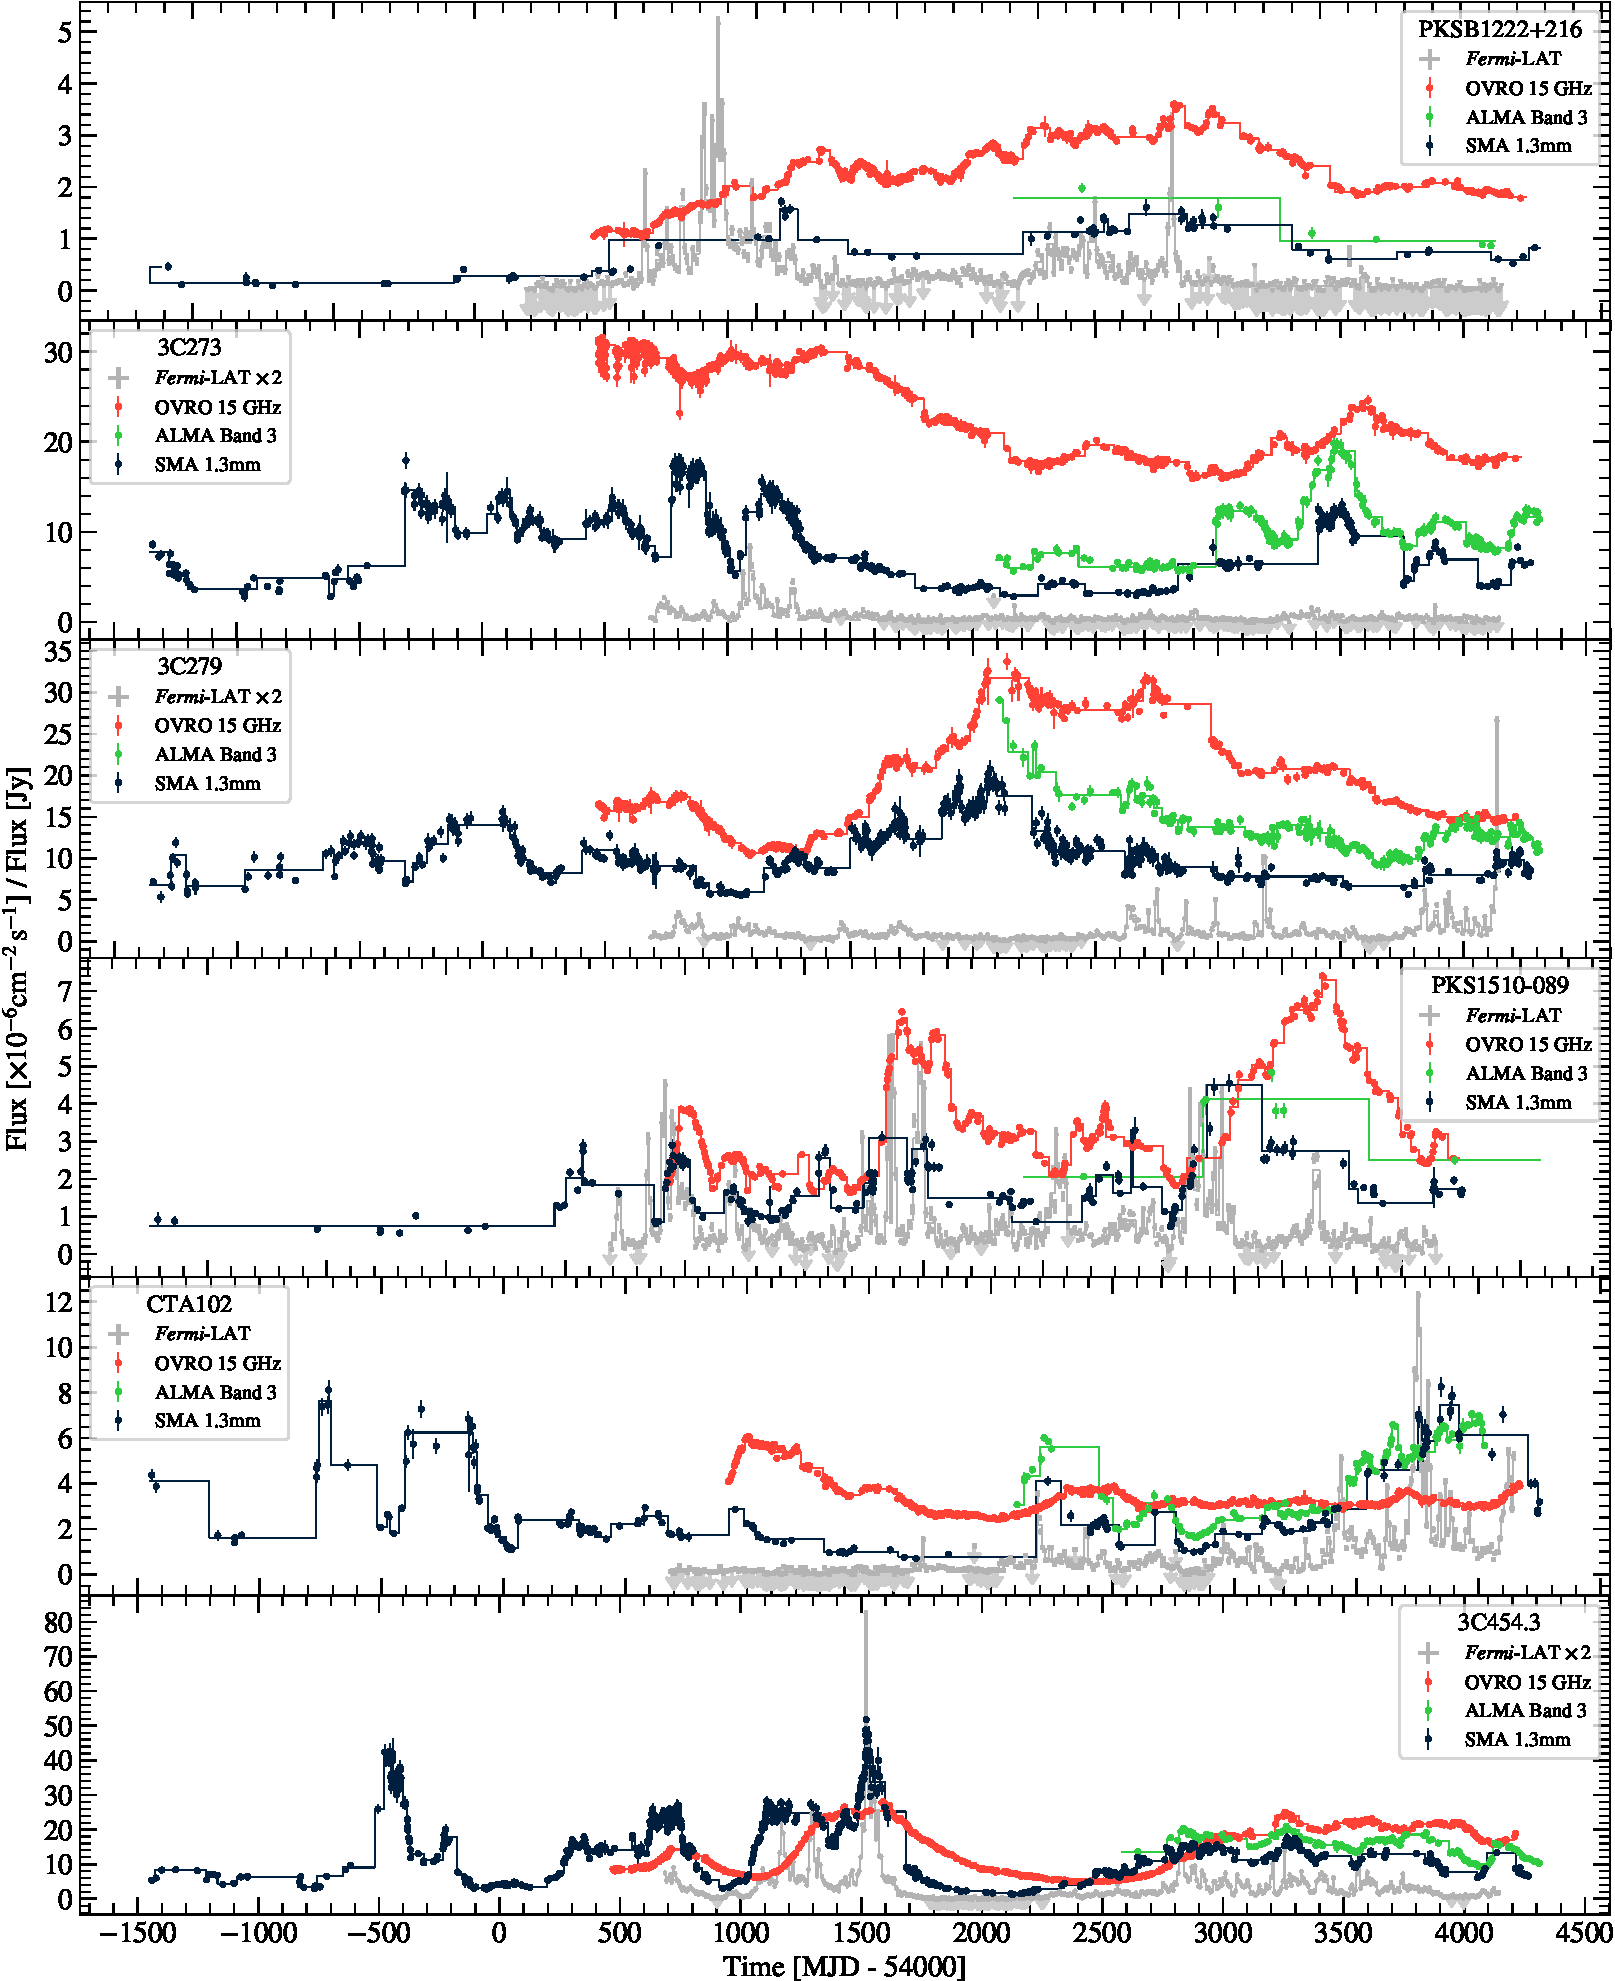
\includegraphics[width = .8\linewidth]{figures/lc_gamma_radio_tsmin9.pdf}
    \caption{Radio and \gray light curves normalized to the respective maximum flux.}
    \label{fig:lc-radio}
\end{figure*}

To quantify the correlations, we again closely follow the methodology laid out by \citet{2014MNRAS.445..437M}. 
For two light curves with fluxes $a_i$ and $b_j$ 
%and uncertainties $\sigma_{ai}$ and $\sigma_{bj}$ 
measured at times $t_{ai}$ and $t_{bj}$ we compute the local cross correlation function
\begin{equation}
\mathrm{LCCF}(\tau) = \frac{1}{M}\frac{\sum(a_i - \bar{a}_\tau)(b_j - \bar{b}_\tau)}{\sigma_{a\tau}\sigma_{b\tau}},
\end{equation}
where the sum runs over the $M$ pairs for which $\tau \leqslant t_{ai} - t_{bj} < \tau + \Delta t$, for some chosen time step $\Delta t$, and $\bar{a}_\tau$ and $\bar{b}_\tau$ and $\sigma_{a\tau}$ and $\sigma_{b\tau}$ are the flux averages and standard deviations over the $M$ pairs, respectively~\citep{1999PASP..111.1347W}. 
The LCCF is bound between $-1$ and $1$ and has much larger efficiency in recovering linear correlations between light curves compared to the discrete correlation function \citep{2014MNRAS.445..437M}.
%We also prefer this method over the $Z$-tranformed DCF used in Section~\ref{sec:tcool} because it is possible to assign a significance to a time lag corresponding to the maximum value of the LCCF as outlined below. 
For the binning of the time lags $\tau$ we choose half the maximum of the median of the time separations between consecutive data points in the two light curves.
The minimum and maximum values of $\tau$ are chosen to be $\pm0.5$ times the length of the shortest light curve~\citep{2014MNRAS.445..428M}.

We determine the significance of a peak in the LCCF by cross correlating pairs of simulated light curves. 
For the \gray light curves, the simulation proceeds in the same way as described in Section~\ref{sec:results-global}, where we use the best-fit values $\hat{\beta}$ for the assumed PSDs.
For the radio light curves, we proceed in a similar way. 
First, we determine the best-fit PSDs similar to the \gray light curves. 
In order to achieve a good fit between the observed and simulated PSDs we change the methodology used for the \gray light curves in the following ways:
instead of matching the flux PDFs of the light curves as suggested by \citet{2013MNRAS.433..907E}, we use variance matching~\citep{2014MNRAS.445..437M}.\footnote{For radio light curves, the best-fit slopes are much closer to $\beta \sim 2$, so that Parseval's theorem applies.}
Furthermore, we do not apply uncertainties to the simulated light curves. 
Doing so generally leads to a strong flattening of the periodograms at high frequencies when they become dominated by white noise introduced by the uncertainties. 
This is not observed in the periodogram derived from observations. 
The reason might be a correlation between uncertainties and flux, which is not taken into account by the adopted simulation scheme, and which can lead to an overestimation of the simulated uncertainties.
Lastly, the radio light curves are unevenly sampled and can show large observational gaps. 
Simply applying the interpolation scheme used for the the \gray light curves would mean that most data points that enter the calculation of the periodogram are actually interpolated. 
To mitigate this problem, we split the light curves where they show large gaps. 
We found that a split at gaps that are 20 (4.5) times larger than the median separation between consecutive measurements for OVRO and SMA (ALMA) light curves provides a good compromise between minimizing the number of splits and too few data points within a light curve segment. 
Furthermore, for the interpolated light curves we use a time step equal the 80\,\% quantile of the observed separation (the median would correspond to the 50\% quantile). 
In this way, we loose sensitivity to the highest frequencies but end up with interpolated light curves with roughly the same number of data points as the observed ones. 
We do not average the interpolated flux points as in the \gray case since radio observations are usually short in duration and report flux densities instead of integrated fluxes. 
The periodograms of the individual light curve segments are finally log averaged following \citet{1993MNRAS.261..612P}.

We report the best-fit slopes of the assumed power-law PSDs $\hat{\beta}$, their confidence interval, and the $p_\beta$-value of the fits in Table~\ref{tab:lccf}.
The confidence interval and $p_\beta$-value are determined in the same way as described in Section~\ref{sec:results-global}.
All fits show a high fit quality. 
For the SMA and OVRO light curves for 3C454.3, as well as for the 3C273 light curve obtained with ALMA, we are only able to provide upper bounds on $\beta$.
In general we confirm the trend that the OVRO light curves show a softer PSD $\hat{\beta} \gtrsim 2$ for all sources. 
Moving to higher frequencies with ALMA and SMA, the PSD hardens and becomes more flicker-noise like. 
Comparing our results for the OVRO light curves to previous analyses of \citet{2014MNRAS.445..428M}, who used 4 years of data, we find them to be consistent within uncertainties. 

Having determined the best-fit PSDs, we use them it to create artificial light curves in the same way as for fitting the periodogram itself.
We then calculate the LCCF between 5000 pairs of un-correlated simulated light curves and derive confidence bands on the LCCF. We use the confidence bands to determine the $p_\tau$-value, which gives the probability to find an LCCF value at given $\tau$ greater or equal to the observed value under the assumption that the light curves are un-correlated. 

For observed LCCFs where we find time lags with a significance $1 - p_\tau > 0.95$, we estimate the uncertainty on the peak time using flux randomization and random subsample selection (drawing 1000 samples) following \citet{1998PASP..110..660P} as suggested by \citet{2014MNRAS.445..437M}.

\begin{deluxetable*}{l|cc|ccc}
\tablewidth{0pt}
\tablecaption{ \label{tab:lccf}Results from PSD analysis of radio light curves as well as \gray and radio LCCF results.}
\tablehead{\colhead{Source} & \colhead{$\hat{\beta}$} & \colhead{$p_\beta$} & \colhead{$\tau_\mathrm{peak}$ [days]} & \colhead{$p_\tau$} & \colhead{$d_{\gamma, r}$ [pc]}}
\startdata
\hline
\multicolumn{6}{c}{OVRO}\\
\hline
PKSB1222+216 & $1.92^{+0.39}_{-0.59}$ & 0.59 & --- & --- & ---\\
3C273 & $2.38^{+0.30}_{-0.97}$ & 0.94 & $-416.5^{+217.0}_{-140.0}$ & 0.0068 & $10.96~[5.2,14.6]~\pm4.4$\\
3C279 & $2.29^{+0.32}_{-0.94}$ & 0.71 & --- & --- & ---\\
PKS1510-089 & $1.89^{+0.45}_{-0.84}$ & 0.34 & --- & --- & ---\\
CTA102 & $2.23^{+0.26}_{-0.92}$ & 0.84 & --- & --- & ---\\
3C454.3 & $2.20^{+0.36}_{-2.20}$ & 0.40 & $-101.5^{+49.0}_{-112.0}$ & 0.0156 & $15.39~[8.0,32.4]~\pm2.8$\\
\hline
\multicolumn{6}{c}{ALMA Band 3}\\
\hline
3C273 & $2.12^{+0.40}_{-2.12}$ & 0.73 & --- & --- & ---\\
3C279 & $1.82^{+0.38}_{-0.45}$ & 0.89 & --- & --- & ---\\
CTA102 & $1.94^{+0.42}_{-1.33}$ & 0.45 & $-216.0^{+209.0}_{-11.0}$ & 0.0092 & $58.85~[1.9,61.8]~\pm7.3$\\
3C454.3 & $1.73^{+0.36}_{-0.30}$ & 0.25 & $-27.0^{+30.0}_{-30.0}$ & 0.0164 & $4.09~[-0.5,8.6]~\pm0.7$\\
\hline
\multicolumn{6}{c}{SMA 1.3mm}\\
\hline
3C273 & $1.48^{+0.40}_{-0.33}$ & 0.17 & $-122.5^{+84.0}_{-7.0}$ & 0.0088 & $3.22~[1.0,3.4]~\pm1.3$\\
3C279 & $1.61^{+0.16}_{-0.28}$ & 0.97 & --- & --- & ---\\
3C454.3 & $1.64^{+0.31}_{-1.64}$ & 0.21 & $10.5^{+21.0}_{-28.0}$ & 0.0002 & $-1.59~[-4.8,2.7]~\pm0.3$\\
\enddata
{
\tablecomments{For the LCCF analysis we only report time lags $< 0 $ and with a significance $p_\tau < 0.05$. The range of $d_{\gamma, r}$ values reported in square brackets is due to the uncertainty on $\tau_\mathrm{peak}$, the remaining uncertainties are the propagated errors on $\Gamma$ and $\delta_\mathrm{D}$.}
}
\end{deluxetable*}

We show the observed LCCF between \gray and radio light curves in Figure~\ref{fig:lccf} for the cases where we find a significant peak in the LCCF. This is the case for 3C273 (OVRO and SMA), CTA102 (ALMA), and 3C454.3 (all radio and mm light curves correlate with the \gray light curve).
The correlation between the SMA and \gray light curve of 3C454.3 is the most significant with $p_\tau = 2\times10^{-4}$ ($3.72\sigma$). 
The peak and the uncertainties are marked by a dotted line and shaded region in Figure~\ref{fig:lccf}.
They are also summarized together with the $p_\tau$ values in Table~\ref{tab:lccf}.
In the table, we only consider peaks with $\tau < 0$ (\gray light curve leads the radio light curve), however, 
for 3C273 and 3C454.3 peaks with $\tau > 0$ are also visible. 
For 3C454.3 these peaks occur at large values of $\tau$ that might be due to the several small flares observed at \gray energies. Since the overlap between the light curves is smaller for larger values of $|\tau|$ we deem these peaks less credible. 
For 3C273 the situation is less clear. 
The SMA light curve shows two prominent flares around the 
\gray flare, which gives rise to the two peaks in the LCCF. 
The low state of the source in recent years and the less dense sampling of the SMA light curve render it difficult to draw firm conclusions. As we see below, even the peak at $\tau < 0$ does not lead to constraints on the position of the \gray emitting region.

\begin{figure*}
    \centering
    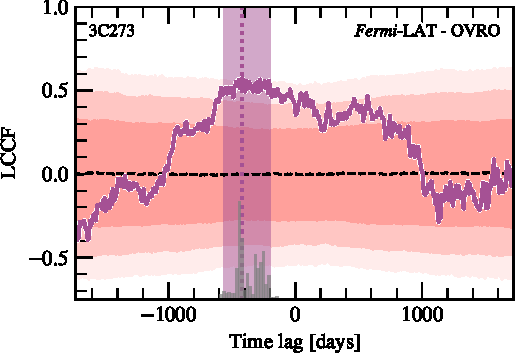
\includegraphics[width = .32\linewidth]{figures/lccf_3C273_nsim5000_fermi_EM13gaps-data_ovro_MM14gaps-none_lccf.pdf}
    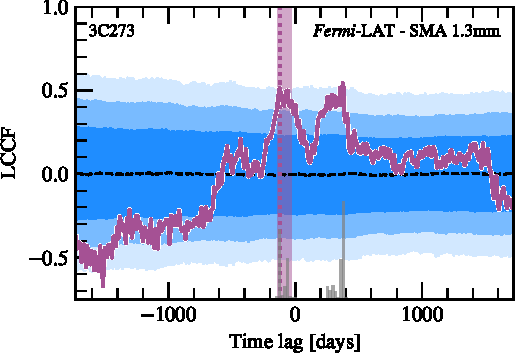
\includegraphics[width = .32\linewidth]{figures/lccf_3C273_nsim5000_fermi_EM13gaps-data_sma-1p3mm_MM14gaps-none_lccf.pdf}
    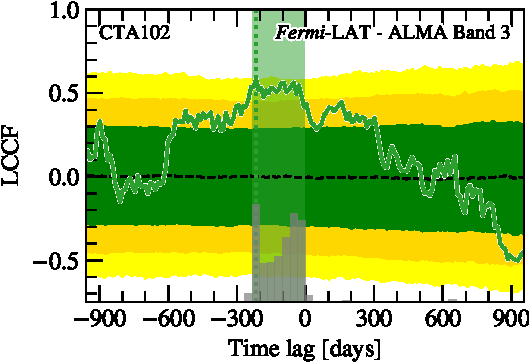
\includegraphics[width = .32\linewidth]{figures/lccf_CTA102_nsim5000_fermi_EM13gaps-data_alma-band3_MM14gaps-none_lccf.pdf}
    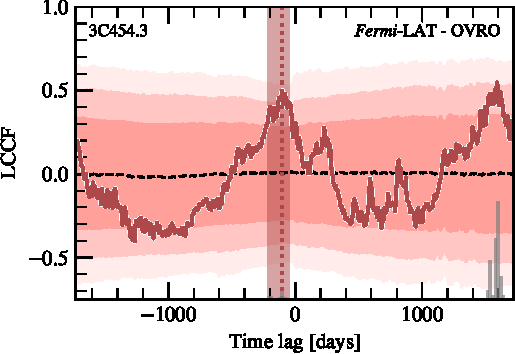
\includegraphics[width = .32\linewidth]{figures/lccf_3C454p3_nsim5000_fermi_EM13gaps-data_ovro_MM14gaps-none_lccf.pdf}
    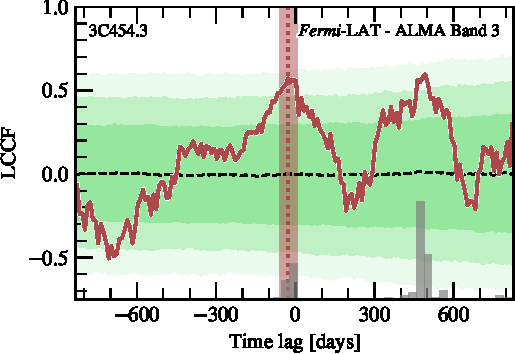
\includegraphics[width = .32\linewidth]{figures/lccf_3C454p3_nsim5000_fermi_EM13gaps-data_alma-band3_MM14gaps-none_lccf.pdf}
    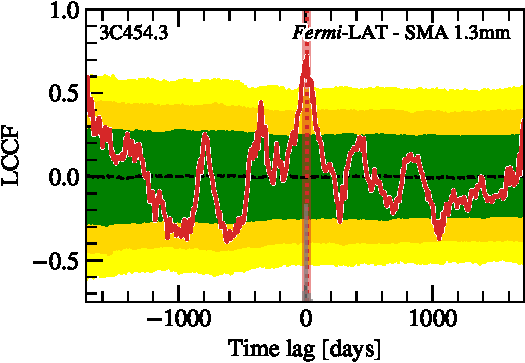
\includegraphics[width = .32\linewidth]{figures/lccf_3C454p3_nsim5000_fermi_EM13gaps-data_sma-1p3mm_MM14gaps-none_lccf.pdf}
    \caption{LCCFs between \gray and radio light curves for the cases where a significant time lag, $p_\tau < 0.05$, is found. The vertical dotted line and shaded regions show the time lag peaks (for $\tau < 0$) and their uncertainty. 
    The the colored regions denote the 68\,\%, 95\,\%, and 99\,\% envelopes (from dark to light) derived from simulated un-correlated light curve pairs. 
    The grey histograms show the number of $\tau_\mathrm{peak}$ values obtained from flux randomization and random subsample selection to estimate the uncertainty on $\tau_\mathrm{peak}$.}
    \label{fig:lccf}
\end{figure*}

Using Eq.~\ref{eq:dgamma-r} and the peaks identified in the LCCF, we can now derive the distance between the \gray and radio emitting region. 
For 3C454.3 the time lags between the \gray and mm light curves of ALMA and SMA are consistent with zero and hence $d_{\gamma,r}$ is consistent with zero as well.
For the correlation with the OVRO light curve, a longer time lag $\tau_{\mathrm{peak},\gamma,15\mathrm{GHz}} = -102$ days is found, placing $d_{\gamma,r}$ between $\sim 5$ and 35\,pc.
This time lag is consistent with the recent DCF analysis carried out by \citet{2018MNRAS.480.5517L} who found a time lag of $(115\pm6)$\,days at $2.5\,\sigma$ significance using 8\,years of OVRO data and the \fermiLAT weekly monitored light curve. 

For CTA102, we only find a significant lag between the ALMA and \gray light curve. 
The time lag translates into $d_{\gamma,r} \sim [-5;69]\,$pc taking uncertainties on $\tau_{\mathrm{peak},\gamma,100\mathrm{GHz}}$ as well as $\Gamma$ and $\delta_\mathrm{D}$ into account.
Hence, the distance is also consistent with zero. 

We also find significant correlation between the \gray light curve of 3C273 and both light curves of SMA and OVRO. 
For the 15\,GHz OVRO light curve $d_{\gamma,r}$ is found between 0.8 and 19\,pc whereas for 230\,GHz the distance falls between $-0.7$ and 4.7\,pc and is consistent with zero. 

In order to determine the core positions at $\sim100$\,GHz (ALMA) and $230\,$GHz core (SMA) we carry out a cross-correlation between the radio light curves to derive $\tau_{\mathrm{peak},15\mathrm{GHz},r\nu}$.
The results are reported in Table~\ref{tab:lccf-radio}.
Using Eqs.~\ref{eq:core-shift1} and \ref{eq:core-shift2} we arrive at the new core position, which we also show in Table~\ref{tab:lccf-radio}, where we use the average values of the measured jet proper motion~\citep[see Table 4 in][]{2016AJ....152...12L}, the observation angle $\theta_\mathrm{obs}$ reported in \citet{2017ApJ...846...98J},
and values $k_r$ found in the dedicated analyses discussed above. 
For 3C273 and 3C454.3 we find that our core positions are consistent with values calculated from the $d_\mathrm{core}\propto\nu^{-1/k_r}$ relation obtained by \citet{2013ARep...57...34V} and \citet{2014MNRAS.437.3396K}, respctively. 
This is a non-trivial result since we have combined our time lags with jet proper motions from MOJAVE and jet properties from VLBA observations. 

Combining the core positions and $d_{\gamma,r}$ we find that for 3C454.3 the \gray emitting region is consistent with the position of SMA mm core at $\sim 0.8^{+0.4}_{-0.5}$\,pc, also in agreement with the LCCF from ALMA. The OVRO result is only marginal in agreement with this result, suggesting instead that $d_\gamma \gtrsim 3\,$pc.
Given the larger uncertainty on the time lag and lower significance of the correlation, we deem the results at mm wavelegnths as more robust. 
They also agree with the findings of \citet{2014MNRAS.441.1899F}.

For CTA102 we do not find a significant correlation with the OVRO light curve and therefore we use the core position at 86\,GHz, $d_{\mathrm{core},86\,\mathrm{GHz}} \sim 7\,$pc~\citep{2015A&A...576A..43F}.
With the results on $d_{\gamma,r}$ we find that also for CTA102 the distance of the \gray emitting region is consistent with the mm core.

For 3C273, we find that the derived core shift between 230\,GHz and 15\,GHz of $\sim 4\,$pc is not consistent with the $\nu^{-1/1.4}$ relation obtained by \citet[][]{2013ARep...57...34V}. 
Nevertheless, within uncertainties, $d_{\gamma,r}$ is also consistent with zero, and hence \gray and mm emission could be produced co-spatially.

\begin{deluxetable}{lccc}
\tablewidth{0pt}
\tablecaption{ \label{tab:lccf-radio}Results for time lags and core positions from a radio/radio LCCF analysis.}
\tablehead{\colhead{Source} & \colhead{$\tau_{\mathrm{peak},r\nu_1,r\nu_2}$ [days]} & \colhead{$p_{\tau}$}  & \colhead{$d_{\mathrm{core},r\nu_1}$ [pc]}  }
\startdata
\hline
\multicolumn{4}{c}{ALMA Band 3 \& OVRO}\\
\hline
3C273 & $-161^{+72}_{-36}$ & 0.0222 & $1.5~[0.8,1.8]~\pm0.6$ \\
3C279 & $-622^{+154}_{-168}$ & 0.0036 & $8.1~[6.1,10.3]~\pm2.6$ \\
CTA102 & --- & --- & --- \\
3C454.3 & $-667^{+100}_{-30}$ & 0.0782 & $4.6~[3.9,4.8]~\pm2.6$ \\
\hline
\multicolumn{4}{c}{SMA 1.3mm \& OVRO}\\
\hline
3C273 & $-427^{+293}_{-87}$ & 0.0256 & $4.0~[1.2,4.8]~\pm1.5$ \\
3C279 & $-165^{+12}_{-125}$ & 0.0152 & $2.2~[2.0,3.8]~\pm0.7$ \\
3C454.3 & $-110^{+14}_{-0}$ & 0.0924 & $0.8~[0.7,0.8]~\pm0.4$ \\
\hline
\multicolumn{4}{c}{SMA 1.3mm \& ALMA Band 3}\\
\hline
3C273 & $1^{+9}_{-36}$ & 0.0000 & --- \\
3C279 & $-188^{+175}_{-119}$ & 0.0002 & --- \\
3C454.3 & $3^{+10}_{-20}$ & 0.0004 & --- \\
\enddata
{
\tablecomments{For the LCCF analysis we only report time lags and with a significance $p_\tau < 0.1$. The range of core position  in square brackets are due to the uncertainty on $\tau_\mathrm{peak}$, whereas the remaining uncertainties are the propagated errors on $\theta_\mathrm{obs}$ and the jet proper motion $\mu$.}
}
\end{deluxetable}

\section{Summary and Conclusion}
\label{sec:conclusion}

We have carried out a comprehensive temporal and spectral analysis of  \gray data of 6 FSRQs that have exhibited the brightest \gray flares within 9.5 years of \fermiLAT observations.
In order to identify flaring episodes in an objective way, we have introduced a novel combination of Bayesian blocks (BBs)~\citep{2013ApJ...764..167S} and a hill-climbing algorithm inspired by the HOP group finding algorithm~\citep{1998ApJ...498..137E}, see Section~\ref{sec:zoom}.
We have derived daily, orbital, and sub-orbital light curves for the brightest \gray flares identified in this way.

From the weekly-binned full 9.5\,year light curves, we are able to determine global temporal properties (Section~\ref{sec:results-global}) such as the flux distributions and power spectral densities (PSDs). 
The former are well described with broken power laws or log-normal distributions, while the latter, derived following \citet{2014MNRAS.445..437M}, indicate that the light curves show power-law type PSDs with indices $\beta\sim 1$ indicating flicker noise.
We also developed a novel objective algorithm to determine the flux level of the quiescent background (see Section~\ref{sec:qb}).

We use the light curves with one flux bin per orbit to derive local temporal flare properties by fitting the light curves with exponential  profiles (Section~\ref{sec:results-local}).
The obtained rise and decay times show that rapid variability at time scales of the order of the horizon crossing time scale, which range from $\sim 0.5$ to $\sim 2$ \,hours for the considered black hole masses, are a common feature of all sources.
In general, we find a large variety of flares showing both fast-rise and exponential decay (FRED) behavior and the opposite. 
No clear trend between flare asymmetry and other flare parameters such as peak flux, integrated flux, or flare duration is found. 
No apparent evolution of these quantities with time is observed either. 
This variety of flare profiles could be explained in the scheme of magnetic reconnection with different orientations of the reconnection layers leading to a variety of Doppler factors of the injected plasmoids~\citep[e.g.,][]{2016MNRAS.462.3325P,2018MNRAS.tmp.2522C}. 
With our novel approach of identifying flares, it will be possible in the future to build large statistical samples of flares (not only selected by their peak flux but also, e.g., by their integrated flux) whose properties could be compared in more detail to predictions of the reconnection scenario.
Small and fast plasmoids injected closely to the line of sight could also explain minute-scale variability~\citep{2016MNRAS.462.3325P} for which we find evidence at the 2\,$\sigma$ significance level (post-trial) in suborbital light curves of at least two sources, 3C279 and CTA102 (Table~\ref{tab:minute}). 
For 3C454.3 and PKS1510-089, the BBs also indicate variability on such short time scales, however, a fit with a constant flux to light curves of these orbits cannot be rejected beyond the $2\,\sigma$ (post-trial) level.
Other possible explanations of such short variability include an energy-dependent kinetic beaming of particles during reconnection~\citep{2012ApJ...754L..33C}, radiative cooling of a plasma accelerated by re-collimation shocks~\citep{Bodo:2017qqn}, or synchrotron radiation by electrons accelerated to energies beyond $\gamma' \gtrsim 10^6$~\citep{TheFermi-LAT:2016dss}, a scenario motivated by the \gray flares of the Crab nebula~\citep{2011Sci...331..739A} and also discussed for the flare of PKSB1222+216~\citep{2012MNRAS.425.2519N}.
We have proposed two alternative scenarios in which the \Grays are shielded from low energy photons by a plasma sheath (Section \ref{sec:plasma-sheath}) and \Grays produced by synchrotron emission of electron-positron pairs created by the interaction of protons with low energy photons (Section \ref{sec:gammasync}). Our discussion is of qualitative nature only and a full treatment will be presented elsewhere. 

We have also investigated the location of the \gray emitting region  through three approaches: searches for a spectral cut-off, a comparison of decay times with predictions of radiative cooling times, and a correlation between \gray and radio light curves. 
Using the BLR model of \citet{finke2016}, we find no significant spectral cut-off due to the interaction of \Grays with BLR photons, which places the \gray emission region outside or on the edge of the BLR, $r \gtrsim R_{\mathrm{Ly}\alpha}$ or $\gtrsim 10^3r_g$ (see Table~\ref{tab:blrabs}). 
These lower limits are conservative in the sense that more sophisticated models of the BLR~\citep[e.g.,][]{2017MNRAS.464..152A}, which include continuum emission and a more realistic geometry, predict even larger optical depths than the model used here.
We also do not account for a possible brightening of the BLR emission during \gray flares as found by \citet{2013ApJ...763L..36L}.
The observed spectra over different time periods are provided for completeness in Appendix~\ref{sec:avg-spec}.

The observed decay times of the brightest flares are compatible with radiative cooling times predicted from inverse Compton (IC) scattering of electrons with BLR photons for distances of the \gray emitting regions up to $r\sim 1\,$pc. 
IC scattering with photons of the dust torus yields cooling times of the order of hours for values of $r$ up to the sublimation radius of $\sim 3\,$pc. 
This is only compatible with a subset of the analyzed flares, see Table~\ref{tab:blrabs}.
In order to reconcile cooling times with minute-scale variability, the emission region would have to be close to the obtained lower limits. 
At the same time, the value of $r$ needs to be compatible with the amount of observed \gray emission. The IC emission scales as $\delta_\mathrm{D}^3 / x^2$, where $x^2 = R_\mathrm{li}^2 + r^2$ \citep[see, e.g., Eq. 87 in][]{finke2016}. 
A future comparison of the distance derived from IC emission predicted from multi-wavelength modeling and cooling times could provide further insight into this issue.

In principle, the energy dependence of the observed decay times can be used to distinguish cooling with BLR and dust-torus photons, as proposed by~\citet{2012ApJ...758L..15D}. 
At high electron energies, cooling with BLR photons occurs in the Klein-Nishina regime whereas cooling with dust-torus photons occurs in the Thompson regime (see Figure~\ref{fig:tcool}).
However, the fit of exponential flare profiles to light curves in different energy bands yields inconclusive results since the photon statistics are not sufficient to distinguish between the two scenarios.

We find correlations significant beyond the 2.1\,$\sigma$ level between the \gray light curves and radio light curves for 3C273 (correlations found with OVRO and SMA light curves), CTA102 (with ALMA), and 3C454.3 (with OVRA, ALMA, and SMA). 
The time lags between \gray and mm light curves of ALMA and SMA are consistent with zero, which could indicate a co-spatial production. 
This is consistent with the picture of superluminal knots passing through a standing shock associated with the radio core as argued for the flares in PKS1510-089 and 3C454.3~\citep{2010ApJ...710L.126M,2012ApJ...758...72W,2013MNRAS.428.2418O}. 
This would entail values of $r$ at the order of parsecs. 
One has to keep in mind, however, that the inferred  uncertainties on the time lags are large. 
Taken together with the uncertainties on the Doppler boost and bulk Lorentz factor, 
smaller values of $r$ cannot be ruled out by our analysis. 

Our three approaches to constrain the location of the \gray emitting region are all consistent with rather large distances from the central black hole, $r \sim 1\,$pc. 
If the distances are even larger, the radiative cooling with BLR photons becomes inefficient and cooling through IC scattering with dust-torus photons does not reproduce the observed flare decay times. 
Such large distances are at odds with the evidence with minute-scale variability, which we, however, only observe at $\sim2\,\sigma$ post trial significance in the rising parts of the flares. 
Densely sampled light curves at other wavelenghts could provide further insight if this short variability is indeed present and possibly connected to the injection of relativistic particles.
As noted by~\citet{2018MNRAS.477.4749C}, the fact that we do not find significant absorption provides furthermore promising prospects to detect these sources with future observations with the Cherenkov Telescope Array (CTA). 
The improved point source sensitivity of CTA together with its energy range between 20\,GeV and 300\,TeV~\citep{2017arXiv170907997C} could lead to the detection of spectral absorption features during FSRQ flares due to the interaction of \Grays with infrared photons from the dust torus which should become important at $~\sim$TeV energies~\citep[see, e.g., Figure 14 in][]{finke2016}.
CTA observations could further effectively probe the shortest variability time scales at very-high \gray energies.

\begin{acknowledgments}
The \textit{Fermi} LAT Collaboration acknowledges generous ongoing support
from a number of agencies and institutes that have supported both the
development and the operation of the LAT as well as scientific data analysis.
These include the National Aeronautics and Space Administration and the
Department of Energy in the United States, the Commissariat \`a l'Energie Atomique
and the Centre National de la Recherche Scientifique / Institut National de Physique
Nucl\'eaire et de Physique des Particules in France, the Agenzia Spaziale Italiana
and the Istituto Nazionale di Fisica Nucleare in Italy, the Ministry of Education,
Culture, Sports, Science and Technology (MEXT), High Energy Accelerator Research
Organization (KEK) and Japan Aerospace Exploration Agency (JAXA) in Japan, and
the K.~A.~Wallenberg Foundation, the Swedish Research Council and the
Swedish National Space Board in Sweden.
 
Additional support for science analysis during the operations phase is gratefully
acknowledged from the Istituto Nazionale di Astrofisica in Italy and the Centre
National d'\'Etudes Spatiales in France. This work performed in part under DOE
Contract DE-AC02-76SF00515.

The Submillimeter Array is a joint project between the Smithsonian Astrophysical Observatory and the Academia Sinica Institute of Astronomy and Astrophysics and is funded by the Smithsonian Institution and the Academia Sinica.

This research has made use of data from the OVRO 40-m monitoring program~\citep{2011ApJS..194...29R} which is supported in part by NASA grants NNX08AW31G, NNX11A043G, and NNX14AQ89G and NSF grants AST-0808050 and AST-1109911.
\end{acknowledgments}

\begin{appendix}

\section{Average spectra for different time intervals}
\label{sec:avg-spec}
In Table~\ref{tab:avg-spec} we present the average observed best-fit spectra for the analyzed FSRQs for different time ranges. 
The same spectral shapes as in the 3FGL are assumed which are either a log-parabola or a power law with super-exponential cut-off, which are given by
\begin{eqnarray}
    \frac{\mathrm{d}N_\mathrm{LP}}{\mathrm{d}E} = N_0 \left(\frac{E}{E_0}\right)^{-(\Gamma + \kappa\ln(E / E_0))}, \label{eq:avg-spec-lp}\\
    \frac{\mathrm{d}N_\mathrm{PLsupExp}}{\mathrm{d}E} = N_0 \left(\frac{E}{E_0}\right)^{-\Gamma}\exp\left(-\left[\frac{E}{E_\mathrm{cut}} \right]^{\Gamma_2}\right)\label{eq:avg-spec-plexp}.
\end{eqnarray}

\startlongtable
\begin{deluxetable}{ccccccccc}
\tablewidth{0pt}
\tablecaption{ \label{tab:avg-spec}Average spectral parameters for the complete time ranges over which the light curves are derived.}
\tablehead{\colhead{$t_0$} & \colhead{$\Delta t$}  & \colhead{$F(E \geqslant0.1\,\mathrm{GeV})$} & \colhead{$N_0$} & \colhead{$\Gamma$} & \colhead{$\kappa$} & \colhead{$E_\mathrm{cut}$} & \colhead{$\Gamma_2$} & \colhead{$E_0$} \\
\colhead{MJD} & \colhead{days} & \colhead{$[10^{-6}\,\mathrm{cm}^{-2}\,\mathrm{s}^{-1}]$} & \colhead{$[10^{-9}\,\mathrm{MeV}^{-1}\,\mathrm{cm}^{-2}\,\mathrm{s}^{-1}]$} & & & \colhead{[GeV]} & & \colhead{[GeV]}} 
\startdata
\hline
\multicolumn{9}{c}{\textit{Daily light curves}}\\
\multicolumn{9}{c}{PKSB1222+216}\\
 \hline
55088.65  & 35.00 & $0.866\pm0.040$ &  $0.948\pm0.037$ & $2.063 \pm 0.053$ & $0.042 \pm 0.021$ & $\ldots$ & $\ldots$ & 0.31\\
55249.65  & 259.00 & $1.557\pm0.018$ &  $1.707\pm0.018$ & $2.117 \pm 0.014$ & $0.064 \pm 0.006$ & $\ldots$ & $\ldots$ & 0.31\\
56915.65  & 98.00 & $0.815\pm0.026$ &  $0.849\pm0.024$ & $2.298 \pm 0.038$ & $0.074 \pm 0.021$ & $\ldots$ & $\ldots$ & 0.31\\
\hline
\multicolumn{9}{c}{3C273}\\
 \hline
55004.65  & 189.00 & $1.196\pm0.022$ &  $2.038\pm0.034$ & $2.409 \pm 0.027$ & $0.116 \pm 0.016$ & $\ldots$ & $\ldots$ & 0.25\\
55242.65  & 56.00 & $1.070\pm0.043$ &  $1.834\pm0.064$ & $2.360 \pm 0.058$ & $0.107 \pm 0.031$ & $\ldots$ & $\ldots$ & 0.25\\
\hline
\multicolumn{9}{c}{3C279}\\
 \hline
56733.65  & 70.00 & $1.325\pm0.034$ &  $1.148\pm0.027$ & $2.158 \pm 0.028$ & $0.076 \pm 0.015$ & $\ldots$ & $\ldots$ & 0.34\\
57174.65  & 42.00 & $3.078\pm0.054$ &  $2.783\pm0.046$ & $2.082 \pm 0.020$ & $0.095 \pm 0.011$ & $\ldots$ & $\ldots$ & 0.34\\
57797.65  & 91.00 & $1.396\pm0.034$ &  $1.243\pm0.027$ & $2.117 \pm 0.024$ & $0.092 \pm 0.013$ & $\ldots$ & $\ldots$ & 0.34\\
58084.65  & 70.00 & $2.964\pm0.078$ &  $2.816\pm0.053$ & $1.969 \pm 0.026$ & $0.111 \pm 0.011$ & $\ldots$ & $\ldots$ & 0.34\\
\hline
\multicolumn{9}{c}{PKS1510-089}\\
 \hline
54892.65  & 42.00 & $2.541\pm0.055$ &  $1.256\pm0.027$ & $2.205 \pm 0.021$ & $0.094 \pm 0.014$ & $\ldots$ & $\ldots$ & 0.45\\
55830.65  & 63.00 & $2.369\pm0.050$ &  $1.145\pm0.023$ & $2.207 \pm 0.019$ & $0.074 \pm 0.012$ & $\ldots$ & $\ldots$ & 0.45\\
55928.65  & 126.00 & $2.001\pm0.048$ &  $0.915\pm0.016$ & $2.311 \pm 0.020$ & $0.090 \pm 0.012$ & $\ldots$ & $\ldots$ & 0.45\\
57090.65  & 49.00 & $2.311\pm0.074$ &  $1.135\pm0.025$ & $2.195 \pm 0.025$ & $0.081 \pm 0.013$ & $\ldots$ & $\ldots$ & 0.45\\
57230.65  & 28.00 & $2.027\pm0.077$ &  $1.119\pm0.035$ & $1.972 \pm 0.035$ & $0.067 \pm 0.016$ & $\ldots$ & $\ldots$ & 0.45\\
\hline
\multicolumn{9}{c}{CTA102}\\
 \hline
57391.65  & 112.00 & $2.031\pm0.033$ &  $2.843\pm0.739$ & $1.936 \pm 0.104$ & $\ldots$ & $3.742 \pm 3.771$ & $0.536 \pm 0.172$ & 0.31\\
57650.65  & 238.00 & $4.241\pm0.029$ &  $5.065\pm0.210$ & $1.931 \pm 0.026$ & $\ldots$ & $8.638 \pm 1.767$ & $0.704 \pm 0.080$ & 0.31\\
57972.65  & 182.00 & $1.925\pm0.028$ &  $8.507\pm11.070$ & $1.682 \pm 0.255$ & $\ldots$ & $0.107 \pm 0.350$ & $0.321 \pm 0.121$ & 0.31\\
\hline
\multicolumn{9}{c}{3C454.3}\\
 \hline
55123.65  & 84.00 & $5.165\pm0.064$ &  $11.102\pm3.312$ & $1.678 \pm 0.070$ & $\ldots$ & $0.210 \pm 0.137$ & $0.388 \pm 0.038$ & 0.41\\
55263.65  & 56.00 & $6.786\pm0.090$ &  $8.840\pm4.906$ & $1.938 \pm 0.134$ & $\ldots$ & $0.543 \pm 0.789$ & $0.404 \pm 0.101$ & 0.41\\
55459.65  & 189.00 & $8.390\pm0.053$ &  $125.464\pm99.276$ & $1.467 \pm 0.102$ & $\ldots$ & $0.002 \pm 0.004$ & $0.231 \pm 0.025$ & 0.41\\
\hline
\\
\multicolumn{9}{c}{\textit{Orbital light curves}}\\
\multicolumn{9}{c}{PKSB1222+216}\\
 \hline
55359.65  & 10.00 & $4.670\pm0.138$ &  $5.396\pm0.144$ & $1.940 \pm 0.035$ & $0.082 \pm 0.015$ & $\ldots$ & $\ldots$ & 0.31\\
56966.65  & 17.00 & $2.364\pm0.090$ &  $2.504\pm0.098$ & $2.260 \pm 0.046$ & $0.079 \pm 0.028$ & $\ldots$ & $\ldots$ & 0.31\\
\hline
\multicolumn{9}{c}{3C273}\\
 \hline
55091.65  & 38.00 & $2.225\pm0.070$ &  $3.814\pm0.110$ & $2.363 \pm 0.045$ & $0.108 \pm 0.025$ & $\ldots$ & $\ldots$ & 0.25\\
\hline
\multicolumn{9}{c}{3C279}\\
 \hline
56748.65  & 8.00 & $3.549\pm0.120$ &  $3.331\pm0.107$ & $2.076 \pm 0.038$ & $0.144 \pm 0.024$ & $\ldots$ & $\ldots$ & 0.34\\
57185.65  & 6.00 & $10.632\pm0.198$ &  $10.215\pm0.189$ & $1.956 \pm 0.022$ & $0.121 \pm 0.013$ & $\ldots$ & $\ldots$ & 0.34\\
58129.65  & 14.00 & $9.092\pm0.163$ &  $8.421\pm0.138$ & $2.035 \pm 0.020$ & $0.105 \pm 0.011$ & $\ldots$ & $\ldots$ & 0.34\\
\hline
\multicolumn{9}{c}{PKS1510-089}\\
 \hline
54908.65  & 14.00 & $3.890\pm0.102$ &  $1.937\pm0.052$ & $2.188 \pm 0.025$ & $0.090 \pm 0.017$ & $\ldots$ & $\ldots$ & 0.45\\
55848.65  & 11.00 & $5.014\pm0.196$ &  $2.472\pm0.087$ & $2.133 \pm 0.036$ & $0.047 \pm 0.019$ & $\ldots$ & $\ldots$ & 0.45\\
55865.65  & 10.00 & $5.898\pm0.195$ &  $2.930\pm0.090$ & $2.188 \pm 0.031$ & $0.087 \pm 0.020$ & $\ldots$ & $\ldots$ & 0.45\\
55971.65  & 28.00 & $4.240\pm0.083$ &  $2.012\pm0.042$ & $2.273 \pm 0.019$ & $0.100 \pm 0.014$ & $\ldots$ & $\ldots$ & 0.45\\
57112.65  & 6.00 & $4.901\pm0.162$ &  $2.533\pm0.079$ & $2.105 \pm 0.031$ & $0.075 \pm 0.018$ & $\ldots$ & $\ldots$ & 0.45\\
57242.65  & 10.00 & $4.043\pm0.166$ &  $2.377\pm0.080$ & $1.859 \pm 0.039$ & $0.077 \pm 0.017$ & $\ldots$ & $\ldots$ & 0.45\\
\hline
\multicolumn{9}{c}{CTA102}\\
 \hline
57427.65  & 25.00 & $3.410\pm0.080$ &  $4.707\pm1.235$ & $1.785 \pm 0.134$ & $\ldots$ & $3.538 \pm 3.425$ & $0.644 \pm 0.241$ & 0.31\\
57732.65  & 37.00 & $9.203\pm0.079$ &  $11.852\pm0.911$ & $1.783 \pm 0.042$ & $\ldots$ & $6.111 \pm 2.083$ & $0.643 \pm 0.095$ & 0.31\\
57789.65  & 13.00 & $6.703\pm0.171$ &  $13.779\pm7.056$ & $1.606 \pm 0.156$ & $\ldots$ & $1.045 \pm 1.696$ & $0.428 \pm 0.133$ & 0.31\\
57860.65  & 5.00 & $4.988\pm0.211$ &  $5.437\pm0.233$ & $1.873 \pm 0.064$ & $\ldots$ & $17.370 \pm 5.938$ & $1.275 \pm 0.623$ & 0.31\\
58127.65  & 22.00 & $3.996\pm0.080$ &  $5.015\pm0.100$ & $1.965 \pm nan$ & $\ldots$ & $3.354 \pm nan$ & $0.817 \pm nan$ & 0.31\\
\hline
\multicolumn{9}{c}{3C454.3}\\
 \hline
55159.65  & 29.00 & $8.889\pm0.158$ &  $10.164\pm4.488$ & $1.843 \pm 0.137$ & $\ldots$ & $0.914 \pm 1.025$ & $0.487 \pm 0.119$ & 0.41\\
55286.65  & 21.00 & $11.062\pm0.135$ &  $9.695\pm4.868$ & $2.030 \pm 0.151$ & $\ldots$ & $1.659 \pm 2.383$ & $0.506 \pm 0.196$ & 0.41\\
55509.65  & 48.00 & $17.918\pm7.110$ &  $402.758\pm155.384$ & $1.288 \pm 0.048$ & $\ldots$ & $0.002 \pm 0.001$ & $0.237 \pm 0.014$ & 0.41\\
55561.65  & 10.00 & $11.888\pm0.248$ &  $145.234\pm551.525$ & $1.569 \pm 0.446$ & $\ldots$ & $0.002 \pm 0.017$ & $0.211 \pm 0.117$ & 0.41\\
\hline
\\
\multicolumn{9}{c}{\textit{Sub-orbital light curves}}\\
\multicolumn{9}{c}{PKSB1222+216}\\
 \hline
55364.68  & 3.42 & $7.907\pm0.281$ &  $9.309\pm0.308$ & $1.853 \pm 0.043$ & $0.092 \pm 0.019$ & $\ldots$ & $\ldots$ & 0.31\\
56972.49  & 2.75 & $4.083\pm0.257$ &  $4.096\pm0.278$ & $2.328 \pm 0.078$ & $0.034 \pm 0.045$ & $\ldots$ & $\ldots$ & 0.31\\
\hline
\multicolumn{9}{c}{3C273}\\
 \hline
55094.74  & 15.29 & $3.231\pm0.128$ &  $5.657\pm0.203$ & $2.273 \pm 0.058$ & $0.116 \pm 0.031$ & $\ldots$ & $\ldots$ & 0.25\\
\hline
\multicolumn{9}{c}{3C279}\\
 \hline
57188.07  & 1.87 & $22.058\pm0.405$ &  $21.570\pm0.436$ & $1.923 \pm 0.023$ & $0.132 \pm 0.014$ & $\ldots$ & $\ldots$ & 0.34\\
56749.87  & 6.87 & $4.695\pm0.162$ &  $4.301\pm0.143$ & $2.116 \pm 0.039$ & $0.130 \pm 0.024$ & $\ldots$ & $\ldots$ & 0.34\\
58133.34  & 5.32 & $15.058\pm0.343$ &  $14.438\pm0.301$ & $1.988 \pm 0.026$ & $0.131 \pm 0.015$ & $\ldots$ & $\ldots$ & 0.34\\
\hline
\multicolumn{9}{c}{PKS1510-089}\\
 \hline
55850.60  & 4.34 & $6.758\pm0.268$ &  $3.490\pm0.134$ & $2.090 \pm 0.036$ & $0.066 \pm 0.021$ & $\ldots$ & $\ldots$ & 0.45\\
54914.79  & 2.69 & $6.795\pm0.291$ &  $3.659\pm0.155$ & $2.062 \pm 0.042$ & $0.090 \pm 0.025$ & $\ldots$ & $\ldots$ & 0.45\\
55867.64  & 2.16 & $10.018\pm0.553$ &  $5.203\pm0.260$ & $2.105 \pm 0.051$ & $0.080 \pm 0.029$ & $\ldots$ & $\ldots$ & 0.45\\
55872.41  & 1.37 & $10.087\pm0.541$ &  $5.692\pm0.322$ & $2.026 \pm 0.053$ & $0.116 \pm 0.035$ & $\ldots$ & $\ldots$ & 0.45\\
57114.16  & 1.42 & $6.200\pm0.342$ &  $3.193\pm0.180$ & $2.156 \pm 0.053$ & $0.103 \pm 0.036$ & $\ldots$ & $\ldots$ & 0.45\\
57243.84  & 4.53 & $6.042\pm0.282$ &  $3.882\pm0.151$ & $1.696 \pm 0.047$ & $0.107 \pm 0.020$ & $\ldots$ & $\ldots$ & 0.45\\
\hline
\multicolumn{9}{c}{CTA102}\\
 \hline
57737.41  & 1.67 & $14.560\pm0.372$ &  $16.714\pm0.939$ & $1.762 \pm 0.065$ & $\ldots$ & $10.473 \pm 3.823$ & $0.932 \pm 0.273$ & 0.31\\
57749.10  & 4.99 & $15.144\pm0.277$ &  $20.082\pm2.754$ & $1.698 \pm 0.079$ & $\ldots$ & $5.071 \pm 2.997$ & $0.643 \pm 0.151$ & 0.31\\
57757.55  & 4.66 & $13.567\pm0.350$ &  $30.027\pm52.650$ & $1.603 \pm 0.416$ & $\ldots$ & $0.902 \pm 5.436$ & $0.363 \pm 0.353$ & 0.31\\
57861.71  & 2.42 & $8.206\pm0.321$ &  $8.939\pm0.370$ & $1.847 \pm 0.054$ & $\ldots$ & $17.767 \pm 5.612$ & $1.327 \pm 0.586$ & 0.31\\
57435.39  & 8.22 & $5.008\pm0.157$ &  $6.068\pm0.841$ & $1.821 \pm 0.109$ & $\ldots$ & $5.733 \pm 3.476$ & $0.857 \pm 0.343$ & 0.31\\
57446.36  & 0.89 & $3.658\pm0.471$ &  $5.723\pm5.589$ & $1.477 \pm 0.612$ & $\ldots$ & $1.735 \pm 4.707$ & $0.761 \pm 0.823$ & 0.31\\
57449.98  & 0.64 & $4.005\pm0.611$ &  $81.278\pm272.361$ & $0.576 \pm 0.827$ & $\ldots$ & $0.019 \pm 0.088$ & $0.361 \pm 0.187$ & 0.31\\
58127.40  & 1.82 & $5.614\pm0.362$ &  $42.578\pm48.687$ & $1.445 \pm 0.275$ & $\ldots$ & $0.042 \pm 0.099$ & $0.324 \pm 0.096$ & 0.31\\
\hline
\multicolumn{9}{c}{3C454.3}\\
 \hline
55516.55  & 8.93 & $37.920\pm0.468$ &  $114.329\pm2.884$ & $1.574 \pm 0.028$ & $\ldots$ & $0.100 \pm 0.000$ & $0.333 \pm 0.008$ & 0.41\\
55166.29  & 5.55 & $14.132\pm0.387$ &  $10.652\pm4.021$ & $1.965 \pm 0.172$ & $\ldots$ & $2.757 \pm 2.926$ & $0.706 \pm 0.334$ & 0.41\\
\hline
\enddata
{
\tablecomments{The light curves for the respective time intervals are shown in Figs.~\ref{fig:daily}, \ref{fig:gti}, and, for the cases where at least one orbital bin is detected with $\mathrm{TS}\geqslant150$, in Figure~\ref{fig:lc_minutes}.
If uncertainties are $nan$, the parameters have been fixed during the fit to achieve convergence.}
}
\end{deluxetable}

\section{Spectral evolution of orbital light curves}
\label{sec:specvar}
The spectral evolution of the orbital light curves for each source is shown in Figure~\ref{fig:specvar}. In each time bin, a power-law spectrum with index $\Gamma$ and integrated flux $F$ is assumed. 

\begin{figure*}
    \centering
    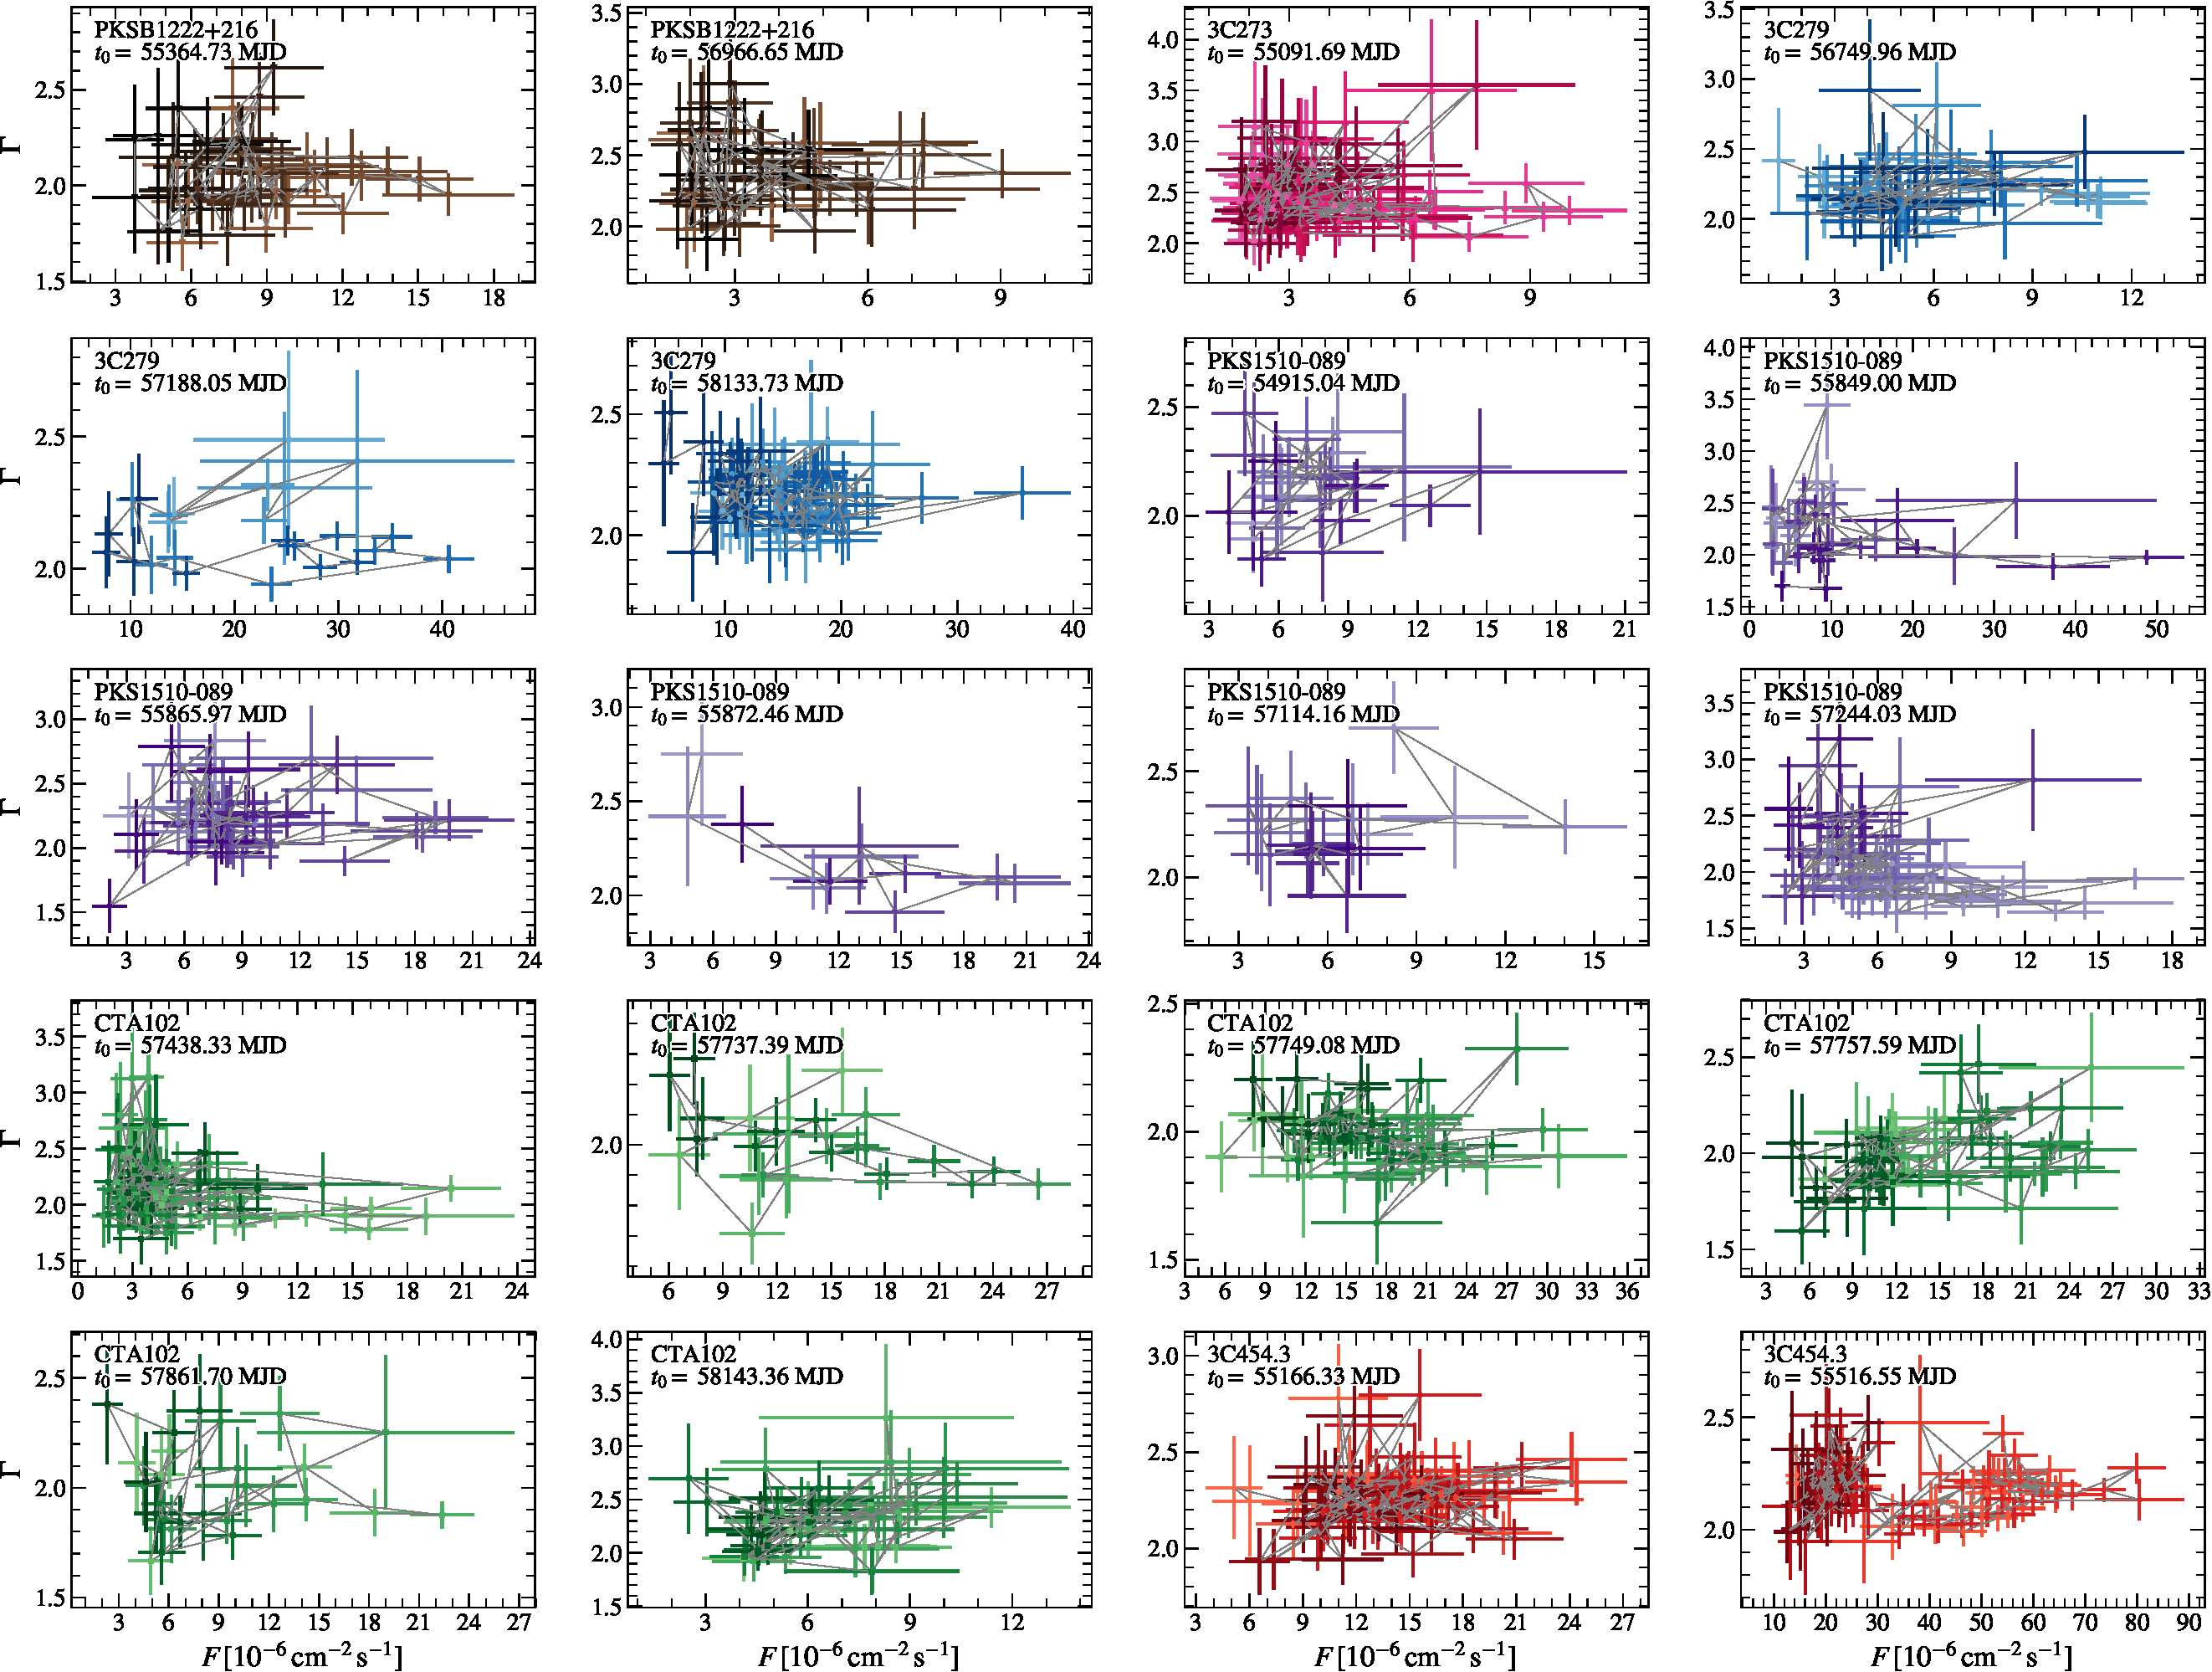
\includegraphics[width = .9 \linewidth]{figures/lc_specvar_flare_int.pdf}
    \caption{Spectral variations of the brightest flares on orbital time scales. Light colors refer to earlier times, dark colors to later times.}
    \label{fig:specvar}
\end{figure*}

\end{appendix}

\bibliography{mainbib}

%% This command is needed to show the entire author+affilation list when
%% the collaboration and author truncation commands are used.  It has to
%% go at the end of the manuscript.
%\allauthors

%% Include this line if you are using the \added, \replaced, \deleted
%% commands to see a summary list of all changes at the end of the article.
%\listofchanges


\end{document}

% End of file `sample62.tex'.
